\documentclass[11pt,a4paper]{article}
\usepackage[margin=2.4cm]{geometry}
\usepackage{amsmath,amssymb,amsthm,mathtools}
\usepackage[protrusion=true,expansion=false]{microtype}
\usepackage{booktabs,enumitem}
\usepackage{placeins}
\usepackage{tikz}
\usetikzlibrary{arrows.meta,positioning,calc,fit,backgrounds}
\definecolor{tierspend}{RGB}{200,60,60}
\definecolor{tierfull}{RGB}{210,140,40}
\definecolor{tierin}{RGB}{60,130,180}
\definecolor{tierrecv}{RGB}{70,150,90}
\usepackage[colorlinks=true,linkcolor=blue!50!black,citecolor=blue!50!black,urlcolor=blue!50!black]{hyperref}

\emergencystretch=3em
\hbadness=10000
\hfuzz=2pt

\newtheorem{theorem}{Theorem}[section]
\newtheorem{lemma}[theorem]{Lemma}
\newtheorem{proposition}[theorem]{Proposition}
\newtheorem{corollary}[theorem]{Corollary}
\theoremstyle{definition}
\newtheorem{definition}[theorem]{Definition}
\newtheorem{construction}[theorem]{Construction}
\newtheorem{assumption}[theorem]{Assumption}
\newtheorem{remark}[theorem]{Remark}
\newtheorem{example}[theorem]{Example}

\newcommand{\F}{\mathbb{F}}
\newcommand{\Z}{\mathbb{Z}}
\newcommand{\N}{\mathbb{N}}
\newcommand{\G}{\mathbb{G}}
\newcommand{\E}{\mathbb{E}}
\newcommand{\PP}{\mathbb{P}}
\renewcommand{\Pr}{\mathrm{Pr}}
\newcommand{\Fp}{\F_p}
\newcommand{\Fq}{\F_q}
\newcommand{\ip}[2]{\langle #1,\, #2 \rangle}
\newcommand{\Comm}{\mathsf{Commit}}
\newcommand{\Open}{\mathsf{Open}}
\newcommand{\Setup}{\mathsf{Setup}}
\newcommand{\Verify}{\mathsf{Verify}}
\newcommand{\negl}{\mathsf{negl}}
\newcommand{\poly}{\mathsf{poly}}
\newcommand{\PPT}{\mathsf{PPT}}
\newcommand{\Adv}{\mathcal{A}}
\newcommand{\Prov}{\mathcal{P}}
\newcommand{\Ver}{\mathcal{V}}
\newcommand{\Sim}{\mathcal{S}}
\newcommand{\Ext}{\mathcal{E}}
\newcommand{\Rel}{\mathcal{R}}
\newcommand{\Lang}{\mathcal{L}}
\newcommand{\nfsym}{\mathsf{nf}}
\newcommand{\cmsym}{\mathsf{cm}}
\newcommand{\cmx}{\mathsf{cmx}}
\newcommand{\cvsym}{\mathsf{cv}}
\newcommand{\rk}{\mathsf{rk}}
\newcommand{\Pallas}{\ensuremath{\mathsf{Pallas}}}
\newcommand{\Vesta}{\ensuremath{\mathsf{Vesta}}}
\newcommand{\Ep}{\ensuremath{\mathcal{E}}}
\newcommand{\NoteCommit}{\ensuremath{\mathsf{NoteCommit}}}
\newcommand{\Sinsemilla}{\ensuremath{\mathsf{Sinsemilla}}}
\newcommand{\ShortCommit}{\ensuremath{\mathsf{ShortCommit}}}
\newcommand{\CommitIvk}{\ensuremath{\mathsf{Commit}^{\mathsf{ivk}}}}
\newcommand{\Extract}{\ensuremath{\mathsf{Extract}}}
\newcommand{\Acc}{\ensuremath{\mathsf{Acc}}}
\newcommand{\GroupHash}{\ensuremath{\mathsf{GroupHash}}}
\newcommand{\ask}{\ensuremath{\mathsf{ask}}}
\newcommand{\aksym}{\ensuremath{\mathsf{ak}}}
\newcommand{\nksym}{\ensuremath{\mathsf{nk}}}
\newcommand{\ivk}{\ensuremath{\mathsf{ivk}}}
\newcommand{\fvk}{\ensuremath{\mathsf{fvk}}}
\newcommand{\ovk}{\ensuremath{\mathsf{ovk}}}
\newcommand{\dk}{\ensuremath{\mathsf{dk}}}
\newcommand{\pkd}{\ensuremath{\mathsf{pk_d}}}
\newcommand{\gd}{\ensuremath{\mathsf{g_d}}}
\newcommand{\rcv}{\ensuremath{\mathsf{rcv}}}
\newcommand{\rcm}{\ensuremath{\mathsf{rcm}}}
\newcommand{\rivk}{\ensuremath{\mathsf{r_{ivk}}}}
\newcommand{\rsk}{\ensuremath{\mathsf{rsk}}}

\renewenvironment{abstract}{%
  \small\begin{center}{\bfseries\abstractname}\end{center}\medskip\noindent\ignorespaces
}{\par\medskip}

\title{\textbf{\Huge Wallet Guide}\\[6pt]\large The Zcash wallet layer: keys, addresses, fees, and transaction construction}
\author{m@rek.onl}
\date{}
\begin{document}
\maketitle
\thispagestyle{empty}
\begin{abstract}
This is the fifth volume of the series --- \emph{Math Guide}, \emph{Crypto
Guide}, \emph{Halo~2 Guide}, \emph{Orchard Guide}, \emph{Wallet Guide}.
Assuming the Orchard protocol of the \emph{Orchard Guide}, it documents the
deployed wallet layer above it: hierarchical key derivation (ZIP-32),
diversified and unified addresses (ZIP-316), the conventional fee (ZIP-317),
the transaction-construction pipeline of \textsf{librustzcash}, partially
created transactions (PCZT), the transaction lifecycle from broadcast through
expiry (ZIP-203), and payment requests (ZIP-321). Every derived quantity
carries its exact derivation, and every claim about deployed behaviour cites
the implementing crate and file.
\end{abstract}
\clearpage
\tableofcontents
\clearpage
\section{Hierarchical key derivation (ZIP-32)}\label{sec:keys-zip32}

The \emph{Orchard Guide} constructs every Orchard key --- $\ask$, $\nksym$,
$\rivk$, the full viewing key, $\ivk$, $\dk$, $\ovk$, and the diversified
addresses --- from a single $32$-byte spending key $\mathsf{sk}$, which it
treats as ``simply a uniform $256$-bit string'', deferring its origin to
ZIP-32 (\S``Keys: capabilities for spending and for viewing'' there,
Definition ``Orchard key hierarchy''). This section supplies that origin. A
deployed wallet does not draw an independent $\mathsf{sk}$ per account: it
draws one \emph{seed} and derives every account's $\mathsf{sk}$ from it
deterministically, so that a single backup recovers every key the wallet
will ever hold. We develop ZIP-32's Orchard instantiation: the hardened-only
derivation tree, the standard account path
$m_{\mathsf{Orchard}} / 32' / \mathit{coin\_type}' / \mathit{account}'$, the
\emph{internal} keys that stand in for a change path level, the fingerprints
that name keys and seeds, and the serialised encodings --- together with
where the deployed stack (\textsf{orchard}, \textsf{zip32},
\textsf{zcash\_keys}, \textsf{zcash\_client\_backend},
\textsf{zcash\_client\_sqlite}) enforces each rule, and where its
documentation and its code disagree.

\subsection{Wallet seeds}\label{sec:zip32-seeds}

The root secret of the whole wallet is a byte string $S$, the \emph{seed}.
ZIP-32 imposes two requirements (ZIP-32, ``Wallet seeds''): the seed MUST be
$32$ to $252$ bytes long, and it MUST be generated with at least $256$ bits
of entropy --- a requirement that extends to any mnemonic phrase from which
the seed is obtained (ZIP-315 gives further guidance). The rationale is the
seed's position in the hierarchy: every key of every account derives
deterministically from $S$, so a lower-entropy seed is a weak link for all
of them at once, and --- unlike an attack on one key --- a brute-force
search over low-entropy seeds runs against many wallets simultaneously.

\begin{remark}[Where the deployed stack enforces the seed bounds]
Enforcement is patchier than the MUST suggests, and one doc comment is
wrong. The derivation function itself does not check: neither
\texttt{ExtendedSpendingKey::master} (\textsf{orchard},
\texttt{src/zip32.rs}) nor \texttt{HardenedOnlyKey::master}
(\textsf{zip32}~0.2.0, \texttt{src/hardened\_only.rs}) inspects the seed
length --- BLAKE2b hashes whatever it is given --- although the former's doc
comment claims ``Panics if the seed is shorter than 32 bytes or longer than
252 bytes''; the claimed panic does not exist. One layer up,
\texttt{UnifiedSpendingKey::from\_seed} (\textsf{zcash\_keys},
\texttt{src/keys.rs}) panics on seeds shorter than $32$ bytes and checks no
upper bound. The trait documentation of \texttt{WalletWrite::create\_account}
and \texttt{import\_account\_hd} (\textsf{zcash\_client\_backend},
\texttt{src/data\_api.rs}) declares a panic for seeds outside $32..252$
bytes, and \textsf{zcash\_client\_sqlite} enforces both bounds ---
indirectly, because it computes a seed fingerprint
(Definition~\ref{def:seed-fingerprint}) via
\texttt{SeedFingerprint::from\_seed}, which returns \texttt{None} outside
$32..252$ bytes (\textsf{zip32}~0.2.0, \texttt{src/fingerprint.rs};
\textsf{zcash\_client\_sqlite}, \texttt{src/lib.rs}). The ZIP requirement
therefore holds at the top of the deployed stack, not in the derivation
function beneath it.
\end{remark}

\subsection{Hardened-only derivation}\label{sec:zip32-hardened}

ZIP-32 obtains Orchard keys by instantiating its generic
\emph{hardened-only key derivation} process with two domain parameters: the
master-key personalisation
$\mathsf{Orchard.MKGDomain} = \texttt{``ZcashIP32Orchard''}$ ($16$ bytes)
and the child-derivation lead byte
$\mathsf{Orchard.CKDDomain} = \mathtt{0x81}$ (ZIP-32, ``Orchard key
derivation''). Non-hardened derivation --- the BIP-32 mode in which a public
key derives child public keys --- is not defined for Orchard at all. That
choice fixes the shape of the extended keys: an \emph{Orchard extended
spending key} is the pair $(\mathsf{sk}, c)$ of a normal $32$-byte spending
key and a $32$-byte \emph{chain code} $c$, and ZIP-32 defines \emph{no}
Orchard extended full viewing key, because with only hardened derivation a
full viewing key confers no child-derivation capability and so has no use
for a chain code (ZIP-32, ``Orchard extended keys''; contrast the Sapling
sections of the same ZIP, which do define extended FVKs). Deployed,
\texttt{ExtendedSpendingKey} carries the pair inside a
\texttt{HardenedOnlyKey} together with bookkeeping fields
\texttt{depth}, \texttt{parent\_fvk\_tag}, and \texttt{child\_index}
(\textsf{orchard}, \texttt{src/zip32.rs}).

\begin{definition}[Orchard master key generation]\label{def:zip32-master}
Given a seed $S$ of $32$ to $252$ bytes, compute
\[
I := \mathrm{BLAKE2b\text{-}512}\bigl(\texttt{``ZcashIP32Orchard''},\ S\bigr),
\qquad I = I_L \,\|\, I_R
\]
with $I_L, I_R$ the first and last $32$ bytes --- unkeyed BLAKE2b-512 with
the $16$-byte personalisation above --- and set
$\mathsf{sk}_m := I_L$, $c_m := I_R$. The \emph{master node} of the Orchard
tree is $m_{\mathsf{Orchard}} := (\mathsf{sk}_m, c_m)$ (ZIP-32,
``Hardened-only master key generation'' instantiated per ``Orchard master
key generation''). Deployed master generation additionally requires
$\mathsf{sk}_m$ to be valid in the sense of
Definition~\ref{def:zip32-validity}, else it fails with
\texttt{Error::InvalidSpendingKey} (\textsf{orchard}, \texttt{src/zip32.rs};
\textsf{zip32}~0.2.0, \texttt{src/hardened\_only.rs}).
\end{definition}

\begin{definition}[Orchard child key derivation]\label{def:zip32-ckd}
Write $i' := i + 2^{31}$ for the \emph{hardened} index derived from
$0 \le i < 2^{31}$ (ZIP-32). Child derivation is defined only for hardened
indices: for $i \ge 2^{31}$,
\begin{gather*}
\mathsf{CKDsk}\bigl((\mathsf{sk}_{\mathrm{par}}, c_{\mathrm{par}}),\ i\bigr):
\quad
I := \mathsf{PRFexpand}_{c_{\mathrm{par}}}\bigl(\mathtt{0x81} \,\|\,
\mathsf{sk}_{\mathrm{par}} \,\|\, \mathrm{I2LEOSP}_{32}(i)\bigr), \\
\mathsf{sk}_i := I_L, \qquad c_i := I_R,
\end{gather*}
where $\mathrm{I2LEOSP}_{32}(i)$ is the $4$-byte little-endian encoding of
$i$ and $\mathsf{PRFexpand}$ is the BLAKE2b-512 expansion function of the
\emph{Orchard Guide} (personalisation \texttt{``Zcash\_ExpandSeed''});
derivation for $i < 2^{31}$ fails (ZIP-32, ``Hardened-only child key
derivation'' and ``Orchard child key derivation'').
\end{definition}

Note the division of labour in the PRF call: the parent \emph{chain code}
$c_{\mathrm{par}}$ is the PRF key, and the parent spending key is message
data. Continuing the tree therefore requires the pair --- the $32$-byte
$\mathsf{sk}$ alone is a leaf capability, which is exactly the property the
account path below exploits when it discards the chain code. Deployed
derivation also caps the depth: the \texttt{depth} field is a byte
incremented with \texttt{checked\_add}, so a child of a depth-$255$ key
cannot exist and the attempt fails with
\texttt{Error::MaxDerivationDepth} (\textsf{orchard},
\texttt{src/zip32.rs}).

\begin{remark}[The general form: triples, and sibling instantiations]
ZIP-32's hardened-only child derivation in full generality takes a triple
$(i, \mathsf{lead}, \mathsf{tag})$ and appends
$\|\, [\mathsf{lead}] \,\|\, \mathsf{tag}$ to the PRF message; each distinct
triple yields an independent output. For $\mathsf{lead} = 0$ and
$\mathsf{tag} = []$ the encoding \emph{omits} both fields, making it
byte-compatible with the earlier definition of $\mathsf{CKDh}$ that lacked
them; Orchard child derivation always uses $\mathsf{lead} = 0$,
$\mathsf{tag} = []$, which is why Definition~\ref{def:zip32-ckd} shows no
such suffix (ZIP-32, ``Hardened-only child key derivation'' and ``Orchard
child key derivation''). ZIP-32 defines no path \emph{notation} for
non-zero $\mathsf{lead}$ or non-empty $\mathsf{tag}$. The deployed encoder
implements the omission literally: \texttt{PrfExpand::with} skips
$[\mathsf{lead}] \,\|\, \mathsf{tag}$ when the lead is zero and the tag
empty (\textsf{zcash\_spec}~0.2.1, \texttt{src/prf\_expand.rs};
\textsf{zip32}~0.2.0, \texttt{src/hardened\_only.rs}). The same
hardened-only process has two sibling instantiations outside the Orchard
tree: \emph{registered} key derivation (personalisation
\texttt{``ZIPRegistered\_KD''}, lead byte $\mathtt{0xAC}$, subtree rooted at
$\mathit{ZipNumber}'$ from an IKM of
$[\mathrm{len}] \,\|\, \mathit{ContextString} \,\|\, [\mathrm{len}] \,\|\, S$)
and the deprecated \emph{ad-hoc} derivation (personalisation
\texttt{``ZcashArbitraryKD''}, lead byte $\mathtt{0xAB}$) (ZIP-32,
``Specification: Registered key derivation'' and ``Specification: Ad-hoc
key derivation (deprecated)''; \textsf{zip32}~0.2.0,
\texttt{src/registered.rs}, \texttt{src/arbitrary.rs}). They matter here
only as neighbours in the domain-separation registry of
Table~\ref{tab:prfexpand}.
\end{remark}

\subsection{The standard account path}\label{sec:zip32-path}

\begin{definition}[Orchard account path]\label{def:zip32-path}
The account-level key for account number
$\mathit{account} \in \{0, \dots, 2^{31}-1\}$ is derived along the path
$m_{\mathsf{Orchard}} / 32' / \mathit{coin\_type}' / \mathit{account}'$:
\[
(\mathsf{sk}_{\mathrm{acct}}, c_{\mathrm{acct}}) :=
\mathsf{CKDsk}\Bigl(\mathsf{CKDsk}\bigl(\mathsf{CKDsk}\bigl(
\mathsf{MKGh}^{\mathsf{Orchard}}(S),\ 32'\bigr),\
\mathit{coin\_type}'\bigr),\ \mathit{account}'\Bigr),
\]
after which the wallet keeps $\mathsf{sk}_{\mathrm{acct}}$ and discards
$c_{\mathrm{acct}}$. The \emph{purpose} level is
$32' = \mathtt{0x80000020}$, registered per BIP~43; the
\emph{coin type} follows the SLIP~44 registry --- $133$ on Mainnet, $1$ on
Testnet and Regtest (all testnets share coin type $1$) --- and accounts are
numbered sequentially from $0$. Wallets MUST support this path for any
account below $2^{31}$ (ZIP-32, ``Key path levels'' and ``Orchard key
path''; coin-type constants deployed in \textsf{zcash\_protocol},
\texttt{src/constants/mainnet.rs}, \texttt{testnet.rs},
\texttt{regtest.rs}).
\end{definition}

The path terminates at the account. Addresses are not further path
children: each account exposes $2^{88}$ diversified addresses per scope,
images of the diversifier indices under FF1 (ZIP-32, ``Orchard key path'';
the construction is in the \emph{Orchard Guide}). Nor is there a change
level between account and address, where BIP-44-style transparent paths put
one: shielded change returning to the originating account is
indistinguishable on-chain from any other output, so a change subtree would
separate nothing an observer can see, and the separation the wallet itself
needs --- telling its own change apart from external receipts --- is
achieved one level lower by the \emph{internal key derivation} of
\S\ref{sec:zip32-internal} (ZIP-32, ``Key path levels'').

\begin{figure}[htbp]
\centering
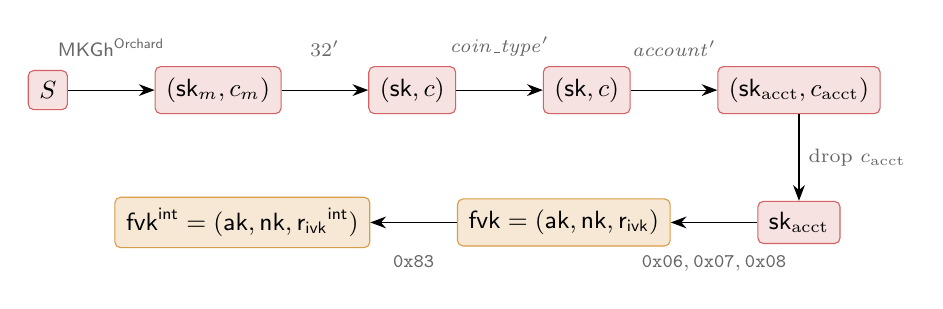
\begin{tikzpicture}[>={Stealth[length=2mm]},
  node distance=11mm and 11mm,
  key/.style={draw, rounded corners=2pt, inner sep=4pt, font=\small},
  spendk/.style={key, fill=tierspend!15, draw=tierspend!80},
  fullk/.style={key, fill=tierfull!20, draw=tierfull!85},
  elab/.style={font=\scriptsize, text=black!60, midway, above=3mm},
  blab/.style={font=\scriptsize, text=black!60, midway, below=3mm},
]
\node[spendk] (S) {$S$};
\node[spendk, right=of S] (M) {$(\mathsf{sk}_m, c_m)$};
\node[spendk, right=of M] (P) {$(\mathsf{sk}, c)$};
\node[spendk, right=of P] (CT) {$(\mathsf{sk}, c)$};
\node[spendk, right=of CT] (A) {$(\mathsf{sk}_{\mathrm{acct}}, c_{\mathrm{acct}})$};
\draw[->] (S) -- node[elab] {$\mathsf{MKGh}^{\mathsf{Orchard}}$} (M);
\draw[->] (M) -- node[elab] {$32'$} (P);
\draw[->] (P) -- node[elab] {$\mathit{coin\_type}'$} (CT);
\draw[->] (CT) -- node[elab] {$\mathit{account}'$} (A);
\node[spendk, below=of A] (SK) {$\mathsf{sk}_{\mathrm{acct}}$};
\draw[->] (A) -- node[right, font=\scriptsize, text=black!60] {drop $c_{\mathrm{acct}}$} (SK);
\node[fullk, left=of SK] (F) {$\fvk = (\aksym, \nksym, \rivk)$};
\node[fullk, left=of F] (FI) {$\fvk^{\mathsf{int}} = (\aksym, \nksym, \rivk^{\mathsf{int}})$};
\draw[->] (SK) -- node[blab] {$\mathtt{0x06}, \mathtt{0x07}, \mathtt{0x08}$} (F);
\draw[->] (F) -- node[blab] {$\mathtt{0x83}$} (FI);
\end{tikzpicture}
\caption{The deployed Orchard key path. Each horizontal arrow in the top
row is one $\mathsf{CKDsk}$ call (Definition~\ref{def:zip32-ckd}): a
$\mathsf{PRFexpand}$ invocation with lead byte $\mathtt{0x81}$, keyed by
the parent chain code. The chain code travels only as far as the account
node $(\mathsf{sk}_{\mathrm{acct}}, c_{\mathrm{acct}})$; the wallet layer
keeps the bare $\mathsf{sk}_{\mathrm{acct}}$, from which the external full
viewing key $\fvk$ (\emph{Orchard Guide}, lead bytes
$\mathtt{0x06}/\mathtt{0x07}/\mathtt{0x08}$) and the internal
$\fvk^{\mathsf{int}}$ (Definition~\ref{def:zip32-internal}, lead byte
$\mathtt{0x83}$) both derive. Red marks spend capability, orange
full-viewing capability, per the series palette.}\label{fig:zip32-path}
\end{figure}

\paragraph{Deployed path derivation.} Function
\texttt{SpendingKey::from\_zip32\_seed(seed, coin\_type, account)}
(\textsf{orchard}, \texttt{src/keys.rs}) rejects
$\mathit{coin\_type} \ge 2^{31}$ with \texttt{Error::InvalidChildIndex},
runs \texttt{ExtendedSpendingKey::from\_path} over the three hardened
indices of Definition~\ref{def:zip32-path}, and returns only the $32$-byte
account spending key --- the chain code is discarded, so the wallet layer
retains no Orchard child-derivation capability below the account level.
Above it, \texttt{UnifiedSpendingKey::from\_seed} stores that plain
\texttt{SpendingKey}, and the unified full viewing key's Orchard component
is the \texttt{FullViewingKey} computed from it (\textsf{zcash\_keys},
\texttt{src/keys.rs}). The \textsf{zip32} crate types the path levels:
\texttt{AccountId} is a $31$-bit integer whose \texttt{TryFrom<u32>}
rejects values at or above $2^{31}$ and which always enters paths hardened,
and \texttt{ChildIndex} is hardened-only --- \texttt{from\_index} returns
\texttt{None} unless the hardened bit is set, and \texttt{hardened(v)}
asserts $v < 2^{31}$ and stores $v + 2^{31}$ (\textsf{zip32}~0.2.0,
\texttt{src/lib.rs}). A distinguished index
$\texttt{ChildIndex::PRIVATE\_USE} = \mathtt{0x7fffffff}'$ is reserved for
private-use subtrees; \textsf{zcashd}'s legacy Sapling account uses it, and
we find no Orchard use (ZIP-32, ``Sapling key path'';
\textsf{zip32}~0.2.0, \texttt{src/lib.rs}).

\subsection{From the account key to addresses: the layer already built}\label{sec:zip32-fvk}

Everything below $\mathsf{sk}_{\mathrm{acct}}$ is the hierarchy the
\emph{Orchard Guide} constructs in ``Keys: capabilities for spending and
for viewing'' (Definition ``Orchard key hierarchy''), and we do not
re-derive it: $\ask$, $\nksym$, $\rivk$ from $\mathsf{PRFexpand}$ lead
bytes $\mathtt{0x06}$, $\mathtt{0x07}$, $\mathtt{0x08}$ with the
$\mathrm{ToScalar}$/$\mathrm{ToBase}$ reductions and their bias analysis;
the sign-canonicalised $\aksym = [\ask]\,G^{\mathsf{SpendAuth}}$;
$\fvk = (\aksym, \nksym, \rivk)$;
$\ivk = \CommitIvk_{\rivk}(\Extract(\aksym), \nksym)$; the
$(\dk, \ovk)$ split of a single $\mathsf{PRFexpand}$ output with lead byte
$\mathtt{0x82}$; and the FF1 diversified addresses with default index $0$
(protocol specification \S4.2.3, ``Orchard Key Components'';
\textsf{orchard}, \texttt{src/keys.rs}).

What ZIP-32 adds at the wallet level is the capability boundary of the full
viewing key. The holder of $\fvk$ obtains, for \emph{both} the external and
the internal scope of \S\ref{sec:zip32-internal}: the incoming viewing keys,
the diversifier keys and outgoing viewing keys, and hence every diversified
address of the account; the \emph{index} behind any of its addresses,
since the diversifier map is a keyed permutation and
$\mathsf{FF1\text{-}AES256}^{-1}_{\dk}(d)$ --- FF1
decryption under the empty tweak --- recovers the index
(\texttt{DiversifierKey::diversifier\_index}, \textsf{orchard},
\texttt{src/keys.rs}); and the scope of any of its
addresses, by trying external then internal
(\texttt{FullViewingKey::scope\_for\_address}, \textsf{orchard},
\texttt{src/keys.rs}). Two contrasts with Sapling sharpen the picture
(ZIP-32, ``Orchard diversifier and OVK derivation''): the diversifier key
derives from the \emph{full viewing key} rather than the extended spending
key, so viewing capability suffices to locate an address's position in the
sequence; and all $2^{88}$ diversifiers are valid, so no rejection loop
exists and the default diversifier is $d_0$. What the full viewing key can
\emph{not} do: derive $\ask$, or derive any child account --- the former by
the one-wayness of the $\mathtt{0x06}$ expansion, the latter because only
hardened derivation exists and no extended FVK is defined
(\S\ref{sec:zip32-hardened}). Finally, no mechanism derives an outgoing
viewing key per \emph{diversified address}: payments are sent from accounts,
with external or internal scope, not from individual addresses (ZIP-32,
``Orchard diversifier and OVK derivation'', citing the ZIP-316 rationale
``Usage of Outgoing Viewing Keys'').

\subsection{Internal keys: change and auto-shielding}\label{sec:zip32-internal}

The path of Definition~\ref{def:zip32-path} reserved no change level, so
the separation between externally visible receiving and wallet-internal
operations --- change outputs, and the auto-shielding of transparent funds
--- happens below the account instead: every account key yields a second,
\emph{internal} full viewing key. The mechanism was implemented in
\textsf{zcashd} as part of ZIP-316 support and applies to keys that are
children of the account level, i.e.\ account keys (ZIP-32, ``Orchard
internal key derivation'').

\begin{definition}[Orchard internal key derivation]\label{def:zip32-internal}
Given an external full viewing key $\fvk = (\aksym, \nksym, \rivk)$, let
$K := \mathrm{LE}_{256}(\rivk)$ and
\begin{gather*}
\rivk^{\mathsf{int}} := \mathrm{ToScalar}\bigl(\mathsf{PRFexpand}_{K}\bigl(
\mathtt{0x83} \,\|\, \mathrm{I2LEOSP}_{256}(\aksym) \,\|\,
\mathrm{I2LEOSP}_{256}(\nksym)\bigr)\bigr) \in \F_{p_{\Vesta}}, \\
\fvk^{\mathsf{int}} := (\aksym, \nksym, \rivk^{\mathsf{int}}),
\end{gather*}
i.e.\ $\mathsf{DeriveInternalFVK}^{\mathsf{Orchard}}$ modifies \emph{only}
$\rivk$ (ZIP-32, ``Orchard internal key derivation''; protocol
specification \S4.2.3). The downstream keys then follow the standard
FVK-level rules of the \emph{Orchard Guide}, applied to
$\fvk^{\mathsf{int}}$:
$\ivk^{\mathsf{int}} := \CommitIvk_{\rivk^{\mathsf{int}}}(\Extract(\aksym), \nksym)$
and $(\dk^{\mathsf{int}}, \ovk^{\mathsf{int}})$ from the $\mathtt{0x82}$
split keyed by $\mathrm{LE}_{256}(\rivk^{\mathsf{int}})$. The
\emph{expanded internal spending key} is
$(\ask, \nksym, \rivk^{\mathsf{int}})$ --- the same $\ask$ --- and no
$32$-byte internal spending key exists (ZIP-32, ``Orchard internal key
derivation'').
\end{definition}

The shape is deliberately that of the $(\dk, \ovk)$ derivation: the same
key $K$, the same message body
$\mathrm{I2LEOSP}_{256}(\aksym) \,\|\, \mathrm{I2LEOSP}_{256}(\nksym)$,
a different lead byte. Its consequences: $\aksym$ and $\nksym$ are
unchanged (the protocol specification notes
$\aksym^{\mathsf{int}} = \aksym$ and $\nksym^{\mathsf{int}} = \nksym$,
\S4.2.3), so spend authorisation and nullifier derivation are common to
both scopes, while $\ivk$, $\dk$, and $\ovk$ all separate because they
derive from $\rivk^{\mathsf{int}}$. The two scopes are therefore two
disjoint families of diversified addresses under one spend authority ---
and since $\ivk^{\mathsf{int}} \ne \ivk$, a note addressed under the
internal scope does not trial-decrypt under the external $\ivk$
(\emph{Orchard Guide}, ``Transmission and detection of a note''), which is
precisely the separation a wallet wants when it hands its external incoming
viewing key to a payment processor. Note that the internal FVK is
\emph{computable from} the external FVK --- the derivation consumes only
$(\aksym, \nksym, \rivk)$ --- so disclosing the full viewing key disclosed
both scopes all along; the boundary runs at the incoming-viewing tier, not
the full-viewing tier. Unlike its Sapling counterpart, the construction
does not rest on non-hardened derivation, which is undefined for Orchard
(ZIP-32, ``Orchard internal key derivation'').

Deployed, the \textsf{zip32} crate's \texttt{Scope} enum
$\{\texttt{External}, \texttt{Internal}\}$ names the two scopes and
\textsf{orchard} re-exports it; \texttt{FullViewingKey::rivk(Scope)},
\texttt{to\_ivk}, \texttt{to\_ovk}, and \texttt{derive\_internal} implement
Definition~\ref{def:zip32-internal} (\textsf{zip32}~0.2.0,
\texttt{src/lib.rs}; \textsf{orchard}, \texttt{src/keys.rs}). The change
path is concrete: \textsf{zcash\_client\_backend} sends Orchard change to
\texttt{ufvk.orchard().address\_at(0u32, Scope::Internal)} --- the
internal-scope address at diversifier index $0$
(\textsf{zcash\_client\_backend}, \texttt{src/data\_api/wallet.rs}).

The transparent pool needs the same external/internal $\ovk$ split ---
its auto-shielding transactions carry shielded outputs whose outgoing
ciphertexts want a viewing key --- but P2PKH keys have no protocol-level
$\ovk$ to scope, so ZIP-316 synthesises the pair.

\begin{definition}[Transparent internal and external OVK]%
\label{def:zip32-transparent-ovk}
For a transparent P2PKH account with BIP-32 account-level extended public
key $(c, pk)$ --- chain code $c$, keying $\mathsf{PRFexpand}$ as a
$256$-bit key, and $\mathsf{ser}(pk)$ the $33$-byte compressed public
key ---
\[
I_{\ovk} := \mathsf{PRFexpand}_{c}\bigl(\mathtt{0xd0} \,\|\,
\mathsf{ser}(pk)\bigr),
\qquad
\ovk_{\mathrm{external}} := I_{\ovk}[0..32),
\quad
\ovk_{\mathrm{internal}} := I_{\ovk}[32..64)
\]
(ZIP-316, \emph{Deriving Internal Keys}; lead byte in
Table~\ref{tab:prfexpand}).
\end{definition}

\begin{remark}[Byte-level normalisation between ZIP and code]
ZIP-32 writes the PRF key as the bit sequence
$\mathrm{I2LEBSP}_{256}(\rivk)$ where $\mathsf{PRFexpand}$ consumes bytes;
the code passes \texttt{rivk.to\_repr()}, the $32$-byte little-endian
encoding. The two are identical under the $\mathrm{LE}_{256}$ convention
this series uses, and we write $\mathrm{LE}_{256}$ throughout, as the
\emph{Orchard Guide} already does. Likewise the $\aksym$ bytes fed to the
$\mathtt{0x82}$ and $\mathtt{0x83}$ messages are
\texttt{SpendValidatingKey::to\_bytes()}, the $32$-byte RedPallas point
encoding --- which, because key generation forces the sign bit to zero (the
canonicalisation of the \emph{Orchard Guide}), coincides with
$\mathrm{I2LEOSP}_{256}(\Extract(\aksym))$, matching the specification's
$\mathrm{I2LEOSP}_{256}(\aksym)$ for
$\aksym \in \{0, \dots, p_{\Pallas}-1\}$ (\textsf{orchard},
\texttt{src/keys.rs}; protocol specification \S4.2.3 and the
$\mathsf{AuthSignPublic}$ type). The $\nksym$ bytes are the base-field
representation.
\end{remark}

\subsection{Key validity and derivation failure}\label{sec:zip32-invalid}

\begin{definition}[Valid Orchard spending key]\label{def:zip32-validity}
A $32$-byte string $\mathsf{sk}$ is a \emph{valid} spending key iff all
three hold: (i) $\ask \ne 0$; (ii) the external
$\ivk = \CommitIvk_{\rivk}(\Extract(\aksym), \nksym) \notin \{0, \bot\}$;
(iii) the internal
$\ivk^{\mathsf{int}} = \CommitIvk_{\rivk^{\mathsf{int}}}(\Extract(\aksym),
\nksym) \notin \{0, \bot\}$. Function \texttt{SpendingKey::from\_bytes}
returns \texttt{None} exactly when one of the three fails
(\textsf{orchard}, \texttt{src/keys.rs}), and the specification's
key-generation algorithm mandates exactly these three discard conditions
--- ``discard this key and repeat with a new $\mathsf{sk}$'' (protocol
specification \S4.2.3, ``Orchard Key Components'').
\texttt{FullViewingKey::from\_bytes} re-checks both scopes when parsing an
FVK from bytes (\textsf{orchard}, \texttt{src/keys.rs}).
\end{definition}

\begin{remark}[Derivation failure has no specified recovery]
ZIP-32 notes that a child spending key may yield an invalid external or
internal full viewing key ``with small probability'' (ZIP-32, ``Orchard
child key derivation'') but prescribes no wallet behaviour when it does;
the specification's ``repeat with a new $\mathsf{sk}$'' addresses a freshly
random key, not a fixed HD path, where there is nothing to redraw. The
deployed stack hard-errors: \texttt{master} and \texttt{derive\_child}
return \texttt{Err(Error::InvalidSpendingKey)},
\texttt{from\_path} propagates it, and \textsf{zcash\_keys} surfaces it as
\texttt{DerivationError::Orchard} (\textsf{orchard}, \texttt{src/zip32.rs};
\textsf{zcash\_keys}, \texttt{src/keys.rs}); no layer implements a
skip-to-next-index convention. This behaviour is normative in practice: an
account index at which derivation fails simply has no key, and no deployed
convention reassigns it. The event is negligibly rare --- neither ZIP-32
nor the specification quantifies ``small probability'', so
Proposition~\ref{prop:zip32-invalid} derives a bound --- and the gap is
theoretical.
\end{remark}

\begin{proposition}[Probability of an invalid key]\label{prop:zip32-invalid}
Model the $\mathsf{PRFexpand}$ outputs and the $\GroupHash$-derived
Sinsemilla generators as uniform and independent (the random-oracle model
in which the \emph{Orchard Guide} analyses both primitives). A uniformly
random $32$-byte $\mathsf{sk}$ then fails the conditions of
Definition~\ref{def:zip32-validity} with probabilities
\[
\Pr[\ask = 0] \;<\; 2^{-254}, \qquad
\Pr\bigl[\ivk \in \{0, \bot\}\bigr] \;\le\; 307/p_{\Vesta} \;<\; 2^{-245}
\quad \text{(per scope)},
\]
and is invalid with probability below $2^{-244}$.
\end{proposition}

\begin{proof}
The scalar $\ask$ is the $\mathrm{ToScalar}$ image of the $\mathtt{0x06}$
expansion (the conditional negation that canonicalises $\aksym$ preserves
zeroness), so $\ask = 0$ iff a uniform $512$-bit integer reduces to $0$
modulo $p_{\Vesta}$. Exactly $\lceil 2^{512}/p_{\Vesta} \rceil$ of the
$2^{512}$ inputs do, and $p_{\Vesta} > 2^{254}$ gives
$\lceil 2^{512}/p_{\Vesta} \rceil < 2^{258}$, hence
$\Pr[\ask = 0] < 2^{258} \cdot 2^{-512} = 2^{-254}$.

For $\ivk$, the two memberships separately. \emph{Zero}: conditioned on
the Sinsemilla hash not returning $\bot$, the commitment point is the hash
point plus $[\rivk]\,H_D$ --- the blinding term of the \emph{Orchard
Guide}'s ``Sinsemilla commitment and short commitment'' --- uniform on the
$p_{\Vesta}$-element Pallas group by perfect hiding, $\rivk$ being uniform
up to the $O(2^{-258})$ $\mathrm{ToScalar}$ bias. The extractor sends only
the identity to $0$, because $y^2 = 0^3 + 5$ has no solution in
$\F_{p_{\Pallas}}$ --- $5$ is a non-square there (protocol specification
\S5.4.9.7, note) --- so $\Pr[\ivk = 0] \le 1/p_{\Vesta} < 2^{-254}$.
\emph{Bottom}: the $\bot$ output arises only inside the Sinsemilla hash,
since the blinding addition is complete (\S5.4.8.4). On the $510$-bit
$\CommitIvk$ message --- two $255$-bit field encodings,
$\lceil 510/10 \rceil = 51$ ten-bit chunks --- the hash performs
$2 \cdot 51 = 102$ incomplete additions (\S5.4.1.9). Each fails only when
one operand is the identity or shares the other's $x$-coordinate --- at
most $3$ of the $p_{\Vesta}$ group elements --- so, with each accumulator
modelled as uniform, the union bound gives
$\Pr[\bot] \le 306/p_{\Vesta} < 2^{9} \cdot 2^{-254} = 2^{-245}$, and per
scope $\Pr[\ivk \in \{0, \bot\}] \le 307/p_{\Vesta}$. The internal scope
repeats the argument with the independent $\rivk^{\mathsf{int}}$ (the
$\mathtt{0x83}$ expansion). In total,
$\Pr[\mathsf{sk}\ \text{invalid}] < (1 + 2 \cdot 307) \cdot 2^{-254} <
2^{10} \cdot 2^{-254} = 2^{-244}$.
\end{proof}

The bound makes ZIP-32's ``small probability'' concrete: below $2^{-244}$
per derived key, and below $2^{-242}$ for the union over the four nodes of
the standard account path (master included,
Definition~\ref{def:zip32-master}). Only the $\bot$ term is heuristic, and
it is doubly guarded: any concrete input exhibiting $\bot$ would
constitute a nontrivial discrete-log relation among the Sinsemilla
generators (\emph{Orchard Guide}, the Sinsemilla collision-resistance
proof), so none is expected ever to be observed.

\subsection{Fingerprints and tags}\label{sec:zip32-fingerprints}

Two identifiers name objects of this section without revealing them; both
are BLAKE2b-256 digests with dedicated personalisations.

\begin{definition}[Orchard FVK fingerprint and tag]\label{def:fvk-fingerprint}
For a full viewing key $\fvk = (\aksym, \nksym, \rivk)$, the
\emph{fingerprint} is
\begin{align*}
\mathsf{FVFP}(\fvk) &:= \mathrm{BLAKE2b\text{-}256}\bigl(
\texttt{``ZcashOrchardFVFP''},\ \fvk_{\mathrm{raw}}\bigr), \\
\fvk_{\mathrm{raw}} &:= \mathrm{I2LEOSP}_{256}(\aksym) \,\|\,
\mathrm{I2LEOSP}_{256}(\nksym) \,\|\, \mathrm{I2LEOSP}_{256}(\rivk),
\end{align*}
the digest of the $96$-byte raw FVK encoding $\fvk_{\mathrm{raw}}$
(protocol specification \S5.6.4.4). The \emph{tag} is its first $4$ bytes
and MUST NOT be assumed unique; the master key's parent tag is the $4$
zero bytes (ZIP-32,
``Orchard Full Viewing Key Fingerprints and Tags''). Deployed as
\texttt{FvkFingerprint} and \texttt{FvkTag}; child derivation stamps each
child with \texttt{parent\_fvk\_tag} $=$ the tag of the parent's FVK
(\textsf{orchard}, \texttt{src/zip32.rs}).
\end{definition}

\begin{definition}[Seed fingerprint]\label{def:seed-fingerprint}
For a seed $S$ of $32$ to $252$ bytes, with $[\mathrm{length}(S)]$ its
single length byte,
\[
\mathsf{SeedFP}(S) := \mathrm{BLAKE2b\text{-}256}\bigl(
\texttt{``Zcash\_HD\_Seed\_FP''},\ [\mathrm{length}(S)] \,\|\, S\bigr);
\]
the string form is Bech32m with human-readable part
\texttt{zip32seedfp}, and no short tag is defined; the length prefix was
chosen to match \textsf{zcashd}'s implementation (ZIP-32, ``Seed
Fingerprints''). Deployed, \texttt{SeedFingerprint::from\_seed} returns
\texttt{None} outside the $32..252$-byte bounds (\textsf{zip32}~0.2.0,
\texttt{src/fingerprint.rs}), and \textsf{zcash\_client\_sqlite} uses the
fingerprint to bind each stored account to the seed that produced it
(\textsf{zcash\_client\_sqlite}, \texttt{src/lib.rs}).
\end{definition}

\subsection{Extended-key encoding and test vectors}\label{sec:zip32-encoding}

\begin{definition}[Orchard extended spending key encoding]\label{def:xsk-encoding}
An extended spending key at depth $\mathsf{depth}$, child index $i$
(hardened offset included), with parent tag $\mathsf{tag}_{\mathrm{par}}$,
serialises as the $73$-byte string
\[
\mathsf{xsk} := \mathrm{I2LEOSP}_{8}(\mathsf{depth}) \,\|\,
\mathsf{tag}_{\mathrm{par}} \,\|\, \mathrm{I2LEOSP}_{32}(i) \,\|\, c \,\|\,
\mathsf{sk}
\qquad (1 + 4 + 4 + 32 + 32 \text{ bytes}),
\]
with the master key at depth $0$, tag $\mathtt{0x00000000}$, index $0$.
The Bech32 human-readable parts are
\texttt{secret-orchard-extsk-main} (Mainnet) and
\texttt{secret-orchard-extsk-test} (Testnet) (ZIP-32, ``Orchard extended
spending keys'').
\end{definition}

ZIP-32 defines this encoding ``for completeness'' and expects most wallets
to expose only the plain $\mathsf{sk}$ encoding of the protocol
specification (\S5.6.4.5) --- consistent with the deployed stack, which
discards the chain code at the account level
(\S\ref{sec:zip32-path}). Indeed we find \emph{no} deployed
\textsf{librustzcash} code path that emits or parses the Bech32 form: the
$73$-byte layout is exercised only by the \textsf{orchard} crate's
embedded test-vector checks, and \textsf{zcash\_keys} stores the raw
spending key inside the unified spending key encoding (\textsf{orchard},
\texttt{src/zip32.rs}, \texttt{src/test\_vectors/zip32.rs};
\textsf{zcash\_keys}, \texttt{src/keys.rs}). We classify the encoding as
specified but unused in the scanned stack.

\begin{remark}[Test vectors]
The ZIP-32 Orchard vectors live in \textsf{zcash-test-vectors} under
\texttt{orchard\_zip32}; the \textsf{orchard} crate embeds four of them ---
the nodes $m$, $m/1'$, $m/1'/2'$, $m/1'/2'/3'$ from the $32$-byte seed
$\mathtt{0x00}, \dots, \mathtt{0x1f}$ --- each giving $\mathsf{sk}$, $c$,
the $73$-byte $\mathsf{xsk}$, and the FVK fingerprint (ZIP-32, ``Test
Vectors''; \textsf{orchard}, \texttt{src/test\_vectors/zip32.rs},
\texttt{src/zip32.rs}). They do \emph{not} cover the standard path of
Definition~\ref{def:zip32-path}. Separate key-component vectors
($\mathsf{sk} \to \ask, \aksym, \nksym, \rivk, \ivk$ and the internal-scope
components) sit in \texttt{src/test\_vectors/keys.rs}, exercised by the
\texttt{keys.rs} tests.
\end{remark}

\begin{example}[The standard path, worked]\label{ex:zip32-standard-path}
No published vector covers the path of Definition~\ref{def:zip32-path}, so
we compute one, from the embedded vectors' seed
$S = \mathtt{0x00}, \dots, \mathtt{0x1f}$, for Mainnet
($\mathit{coin\_type} = 133$) and account $0$:
\begin{center}
\small
\begin{tabular}{@{}lll@{}}
\toprule
$m$ & $\mathsf{sk}$ &
  \texttt{7eee3c1017870990a3dd6891b82f80be8976c1e7dc20d60817a5e88e8b2cd4b8} \\
 & $c$ &
  \texttt{ab8b7a00509ef20e469b5292b61d474b7cffcb1657924cda720250ae40526677} \\
\addlinespace
$m/32'$ & $\mathsf{sk}$ &
  \texttt{93af0a87c2e4704d8825e145557c6a5d4dcbc9016170e276a2080a2dc9eb0f87} \\
 & $c$ &
  \texttt{6e1e808d410d6d1f84e62e67c8b60e80e5ee4de5021d575c0433a625d609c45c} \\
\addlinespace
$m/32'/133'$ & $\mathsf{sk}$ &
  \texttt{149fcee594a2a03de277ab919f22611d0ef6aa8e8e9a0bef32f01a0bcb0e8c4c} \\
 & $c$ &
  \texttt{07d13fdeccd21da16b467f8e785edc32f74ceeb541bede0394647f10fdb7114f} \\
\addlinespace
$m/32'/133'/0'$ & $\mathsf{sk}$ &
  \texttt{b67d8d87cab9189500afb45dbca9f92c924c1de9d9ee1451be4a78313cb223b4} \\
 & $c$ &
  \texttt{7ff0a6392e144d4c8f45bca21fb7827b508446ac069890aefbebbe388b7a84c0} \\
\bottomrule
\end{tabular}
\end{center}
The bottom $\mathsf{sk}$ is exactly what
\texttt{SpendingKey::from\_zip32\_seed} returns for $(S, 133, 0)$; the
bottom $c$ is what it discards. The account key's FVK fingerprint
(Definition~\ref{def:fvk-fingerprint}) is
\begin{center}
\small
\texttt{da8dab741dc4f6ff8964fbaa8840270caf47d286e9a0722e6c89e7f2c38189d5}
\end{center}
(tag $\mathtt{da8dab74}$), its parent's fingerprint begins
$\mathtt{7010c19b}$, and the account's $73$-byte encoding of
Definition~\ref{def:xsk-encoding} is therefore
\[
\mathsf{xsk} = \mathtt{03} \,\|\, \mathtt{7010c19b} \,\|\,
\mathtt{00000080} \,\|\, c \,\|\, \mathsf{sk},
\qquad \mathtt{00000080} = \mathrm{I2LEOSP}_{32}(0'),
\]
with $c$ and $\mathsf{sk}$ the bottom table row. The numbers are
script-computed per the series conventions: a standalone reimplementation
of $\mathsf{MKGh}^{\mathsf{Orchard}}$ and $\mathsf{CKDsk}$ first
reproduces all four embedded vectors byte for byte ($\mathsf{sk}$, $c$,
$\mathsf{xsk}$); the \textsf{orchard} crate, driven as a library,
reproduces their FVK fingerprints, returns the same account $\mathsf{sk}$
from \texttt{from\_zip32\_seed}, and validates every node above per
Definition~\ref{def:zip32-validity}.
\end{example}

\subsection{The $\mathsf{PRFexpand}$ lead-byte registry}\label{sec:zip32-registry}

One PRF underlies every derivation above and in the \emph{Orchard Guide},
but domain separation is per PRF \emph{key}, not protocol-wide: under a
fixed key, distinct lead bytes make the derived secrets mutually
independent, while separate consumers may reuse a byte under different
keys. Sapling derives $\rcm$ and $\mathsf{esk}$ from lead bytes
$\mathtt{0x04}$ and $\mathtt{0x05}$ with no $\rho$ suffix --- the
assignment swapped relative to Orchard's, which the specification
attributes to an oversight (protocol specification \S4.7.3, note) --- and
the Sapling
instantiation of ZIP-32 intentionally reuses
$\mathtt{0x00}$--$\mathtt{0x02}$ from the Sapling key components under a
different key. Table~\ref{tab:prfexpand} collects the accounting for the
Orchard, Orchard-ZIP-32, and ZIP-316 bytes this series constructs; the
Sapling-only bytes ($\mathtt{0x00}$--$\mathtt{0x03}$,
$\mathtt{0x10}$--$\mathtt{0x18}$, of which
\S\ref{sec:addresses-diversified} cites $\mathtt{0x10}$ and
$\mathtt{0x16}$) are accounted in the specification's list (protocol
specification, the $\mathsf{PRF}^{\mathsf{expand}}$ accounting under
``Pseudo Random Functions'' and \S4.2.3; ZIP-32;
\textsf{zcash\_spec}~0.2.1, \texttt{src/prf\_expand.rs}). The Sprout
instantiation of ZIP-32 reserves,
permanently, the lead byte $\mathtt{0x80}$, the personalisation
\texttt{``ZcashIP32\_Sprout''}, and the HRPs
\texttt{zxsprout}/\texttt{zxtestsprout} (ZIP-32, ``Values reserved due to
previous specification for Sprout''). All Orchard and ZIP-32 constants in
this section match between the specification text and
\textsf{zcash\_spec}~0.2.1 --- the version locked by both the
\textsf{orchard} and \textsf{librustzcash} workspaces
(\texttt{Cargo.lock} in each; likewise \textsf{zip32}~0.2.0).

\begin{table}[htbp]
\centering
\small
\begin{tabular}{@{}llll@{}}
\toprule
Lead byte & PRF key & Message after the lead byte & Output \\
\midrule
$\mathtt{0x04}$ & $\mathsf{rseed}$ & $\rho$ & $\mathsf{esk}$ \\
$\mathtt{0x05}$ & $\mathsf{rseed}$ & $\rho$ & $\rcm$ \\
$\mathtt{0x06}$ & $\mathsf{sk}$ & --- & $\ask$ \\
$\mathtt{0x07}$ & $\mathsf{sk}$ & --- & $\nksym$ \\
$\mathtt{0x08}$ & $\mathsf{sk}$ & --- & $\rivk$ \\
$\mathtt{0x09}$ & $\mathsf{rseed}$ & $\rho$ & $\psi$ \\
$\mathtt{0x80}$ & \multicolumn{3}{l}{Sprout ZIP-32 child (reserved; never reuse)} \\
$\mathtt{0x81}$ & $c_{\mathrm{par}}$ &
  $\mathsf{sk}_{\mathrm{par}} \,\|\, \mathrm{I2LEOSP}_{32}(i)$ &
  $\mathsf{sk}_i \,\|\, c_i$ \\
$\mathtt{0x82}$ & $\mathrm{LE}_{256}(\rivk)$ (per scope) &
  $\aksym \,\|\, \nksym$ & $\dk \,\|\, \ovk$ \\
$\mathtt{0x83}$ & $\mathrm{LE}_{256}(\rivk)$ & $\aksym \,\|\, \nksym$ & $\rivk^{\mathsf{int}}$ \\
$\mathtt{0xAB}$ & \multicolumn{3}{l}{ad-hoc ZIP-32 child (deprecated)} \\
$\mathtt{0xAC}$ & \multicolumn{3}{l}{registered ZIP-32 child} \\
$\mathtt{0xD0}$ & $c$ (chain code) & $\mathsf{ser}(pk)$ &
  $\ovk_{\mathrm{ext}} \,\|\, \ovk_{\mathrm{int}}$ \\
\bottomrule
\end{tabular}
\caption{Lead-byte registry of $\mathsf{PRFexpand}$ messages. Point and
field arguments are encoded with $\mathrm{I2LEOSP}_{256}$; $\rho$ is the
$32$-byte nullifier of the Action's spent note (\emph{Orchard Guide},
``Transmission and detection of a note''). Rows
$\mathtt{0x04}$--$\mathtt{0x09}$ are constructed in the \emph{Orchard
Guide} and carry the Orchard meanings of $\mathtt{0x04}$/$\mathtt{0x05}$;
Sapling reuses both bytes, without the $\rho$ suffix and with the outputs
swapped ($\mathtt{0x04} \to \rcm$, $\mathtt{0x05} \to \mathsf{esk}$),
under its own per-note $\mathsf{rseed}$ keys (protocol specification
\S4.7.3, note). Rows $\mathtt{0x81}$ and $\mathtt{0x83}$ are constructed
in
Definitions~\ref{def:zip32-ckd} and~\ref{def:zip32-internal};
$\mathtt{0xD0}$ in Definition~\ref{def:zip32-transparent-ovk};
$\mathtt{0x80}$, $\mathtt{0xAB}$, $\mathtt{0xAC}$ belong
to other subsystems (ZIP-32) and appear for the completeness of
the accounting.}\label{tab:prfexpand}
\end{table}

\section{Diversified and unified addresses (ZIP-316)}\label{sec:addresses}

An address layer must reconcile two demands that pull apart. Each payee
should receive their own address, mutually unlinkable with every other ---
yet all of them spendable by one key and recoverable from one seed; each
shielded protocol solves this with \emph{diversified addresses}. And Zcash
is several protocols at once: transparent, Sapling, and Orchard receivers
coexist, each with its own format, so a recipient wants to hand a sender
\emph{one} string from which the sender's wallet picks the best receiver
both sides support; ZIP-316 solves this above the protocols with the
\emph{unified} container encodings. The \emph{Orchard Guide} (``Keys:
capabilities for spending and for viewing'') already constructs the
Orchard-side machinery --- the key tiers, the FF1-AES256 diversifier map
$d := \mathsf{FF1\text{-}AES256}_{\dk}(d_{\mathrm{plain}})$, the
diversified base
$\gd = \GroupHash^{\Pallas}(\mathtt{z.cash:Orchard\text{-}gd}, d)$, and the
rationale for a keyed permutation over the index space --- and we cite it
throughout. This section adds what the wallet layer builds on top: the
index discipline shared across Sapling, Orchard, and transparent
derivation, the raw and unified encodings, viewing-key containers, and the
deployed address-generation code.

As of this writing ZIP-316 is organised into revisions: Revision~0 is
Active and is what the deployed stack implements; Revision~1 was withdrawn;
Revision~2 is a Draft (ZIP-316, \emph{Revisions}). This volume documents
Revision~0 and states Revision~2 in \S\ref{sec:addresses-r2}, classified
\emph{specified, not deployed}; its reference implementation is
\textsf{librustzcash} PR~\#2199, absent from the deployed crates.
Deployed-behaviour claims below are verified against \textsf{librustzcash}
commit \texttt{62ee526}, the \textsf{orchard} repository at
\texttt{bef8a27}, and the crates-io releases \textsf{zcash\_spec}~0.2.1,
\textsf{zip32}~0.2.0, and \textsf{sapling-crypto}~0.6.0 (exact versions
pinned by the \textsf{librustzcash} workspace \texttt{Cargo.lock}); ZIP
text is
quoted from the \textsf{zips} repository at commit \texttt{c6b7035}.

\subsection{Accounts: ZIP-32 key paths and wallet seeds}\label{sec:addresses-accounts}

Every address below hangs off an \emph{account}, a node of the ZIP-32
hierarchical-deterministic key tree. Sapling and Orchard share the path
shape
\[
m \,/\, \mathtt{purpose}' \,/\, \mathtt{coin\_type}' \,/\,
\mathtt{account}',
\]
with $\mathtt{purpose} = 32'$ ($\mathtt{0x80000020}$), the SLIP-44 coin
type ($133$ on mainnet, $1$ on all testnets), the account index counting
from $0$, and every level hardened (ZIP-32, \emph{Key path levels};
\emph{Sapling key path}; \emph{Orchard key path}; deployed constants in
\textsf{zcash\_protocol}, \texttt{constants/}). Two absences are
deliberate. There is no change level: shielded change pays the wallet's own
address and is indistinguishable from any other output, so the transparent
external/internal split buys nothing (ZIP-32, \emph{Key path levels}). And
there is no non-hardened tail: Orchard ZIP-32 defines hardened-only
derivation, instantiated with
$\mathsf{MKGDomain} = \texttt{"ZcashIP32Orchard"}$ and
$\mathsf{CKDDomain} = \mathtt{0x81}$ over the extended spending key
$(\mathsf{sk}, c)$; a child may, with small probability, yield a spending
key whose external or internal full viewing key is invalid, in which case
derivation at that index simply fails --- ZIP-32 prescribes no recovery,
and the deployed stack surfaces an error (\S\ref{sec:zip32-invalid};
ZIP-32, \emph{Specification: Orchard key derivation}). Wallets MUST
support this path for accounts $0$ to
$2^{31}-1$ and MUST support generating each account's default payment
address; a stream of diversified addresses MAY be supported (ZIP-32,
\emph{Key path levels}; \emph{Sapling key path}; \emph{Orchard key path}).
The seed feeding the tree MUST be $32$--$252$ bytes with at least $256$
bits of entropy: an attack on a lower-entropy mnemonic can be run against
many wallets at once, by matching derived addresses and viewing keys
against observed ones (ZIP-32, \emph{Specification: Wallet seeds}).

\subsection{Diversified addresses}\label{sec:addresses-diversified}

A diversified address multiplies addresses without multiplying keys: one
incoming viewing key $\ivk$, one diversifier key $\dk$, and one $88$-bit
\emph{diversifier} $d$ per address. The \emph{Orchard Guide} (``Keys:
capabilities for spending and for viewing'') constructs the map and its
design rationale --- a keyed permutation of the index space, rather than a
hash or a random draw; the wallet layer fixes the index discipline that
ZIP-32 shares between Sapling and Orchard.

\begin{definition}[Diversifier derivation, Sapling and Orchard]\label{def:diversifier-derivation}
For an account's diversifier key $\dk$, the diversifier at
\emph{diversifier index} $j$ is
\[
d_j := \mathsf{FF1\text{-}AES256.Encrypt}\bigl(\dk,\ \texttt{""},\
\mathrm{I2LEBSP}_{88}(j)\bigr),
\qquad j \in \{0, \dots, 2^{88}-1\},
\]
where $\mathsf{FF1\text{-}AES256}$ is NIST SP 800-38G FF1 with a $256$-bit
AES key, radix $2$, $\mathit{minlen} = \mathit{maxlen} = 88$, and the tweak
always the empty string; input and output are $88$-bit sequences. The
protocol specification abbreviates the keyed permutation as
$\mathrm{PRP}^{d}_{K}(d) := \mathsf{FF1\text{-}AES256}_K(\texttt{""}, d)$
(ZIP-32, \emph{Sapling diversifier derivation}; \emph{Orchard diversifier
and OVK derivation}; protocol specification \S5.4.4, \emph{Pseudo Random
Permutations}).
\end{definition}

The Orchard diversified payment address at index $j$ is then
\[
d := \mathrm{PRP}^{d}_{\dk}\bigl(\mathrm{I2LEBSP}_{88}(j)\bigr),
\qquad
\gd := \mathsf{DiversifyHash}^{\mathsf{Orchard}}(d),
\qquad
\pkd := [\ivk]\,\gd,
\]
the pair $(d, \pkd)$, with the address at index $0$ the \emph{default}
diversified payment address; the last step is the key-agreement
$\mathsf{KA^{Orchard}.DerivePublic}$ of the protocol specification, and the
\emph{Orchard Guide} constructs all three maps. Diversifier indices SHOULD
NOT be chosen at random, and an address generator MAY encode recoverable
information in the index --- the $\dk$ holder recovers it by FF1 decryption
(protocol specification \S4.2.3, \emph{Orchard Key Components}).

The deployed cipher is the \textsf{fpe} crate's \texttt{FF1<Aes256>} at
radix~$2$; the \textsf{orchard} crate pins \textsf{fpe}~0.6 in its
\texttt{Cargo.toml}. Both
protocols encrypt the index bytes \texttt{j.as\_bytes()} wrapped as a
\texttt{BinaryNumeralString} via \texttt{from\_bytes\_le} --- the $11$-byte
little-endian index with bits least-significant-first within each byte,
which is exactly $\mathrm{I2LEBSP}_{88}(j)$ --- under the empty tweak, and
convert the $88$-bit output back with \texttt{to\_bytes\_le}
into the $11$-byte diversifier, exactly $\mathrm{LEBS2OSP}_{88}$
(\textsf{orchard}, \texttt{src/keys.rs}; \textsf{sapling-crypto}~0.6.0,
\texttt{src/zip32.rs}).

The permutation earns its keep quantitatively. An $88$-bit diversifier is
too short to be cryptographically unguessable at the $128$-bit security
level, and diversifiers chosen at random begin to collide by the birthday
bound as the number of draws approaches $2^{44}$; a keyed permutation
reaches the full $2^{88}$ range with no repetition, provided the input
index never repeats for a given node (protocol specification \S5.4.1.6,
notes). The remaining rationale --- per-account sequences pseudorandom and
mutually uncorrelated, and the issue-count leak a bare counter would cause
--- is the \emph{Orchard Guide}'s diversifier construction, cited above.

\begin{remark}[FF1 parameter security]\label{rem:ff1-security}
The property the design requires is that FF1-AES256, with the tweak fixed
to the empty string, is a secure pseudo-random permutation. As
parameterized here --- radix $2$, an $88$-bit domain, $10$ rounds per NIST
SP 800-38G --- it is unaffected by the DKLS2020 attacks on small-domain
FF1: at their parameters $r = 5$ (half the number of rounds) and $n = 44$
(half the domain size in bits), the distinguishing attack has
data complexity $2^{2n((r-1)-1/2)-n} = 2^{264}$ and time complexity
$2^{2n((r-1)-1/2)} = 2^{308}$, no better than brute-forcing the $256$-bit
key (protocol specification \S5.4.4).
\end{remark}

\begin{definition}[Diversifier validity and default diversifiers]\label{def:diversifier-validity}
For Sapling,
\[
\mathsf{DiversifyHash}^{\mathsf{Sapling}}(d) :=
\mathsf{GroupJHash^{URS}}\bigl(\texttt{"Zcash\_gd"},\
\mathrm{LEBS2OSP}_{88}(d)\bigr),
\]
valued in the prime-order subgroup of Jubjub excluding zero, or $\bot$; the
diversifier $d_j$ is \emph{valid} iff the result is not $\bot$, which for a
given $\dk$ holds for approximately half of all indices $j$. The Sapling
\emph{default diversifier} is $d_j$ for the least nonnegative $j$ yielding
a valid diversifier, and a Sapling account has at most approximately
$2^{87}$ payment addresses (ZIP-32, \emph{Sapling diversifier derivation};
\emph{Sapling key path}). For Orchard, with
$P := \GroupHash^{\Pallas}(\mathtt{z.cash:Orchard\text{-}gd},
\mathrm{LEBS2OSP}_{88}(d))$,
\[
\mathsf{DiversifyHash}^{\mathsf{Orchard}}(d) :=
\begin{cases}
\GroupHash^{\Pallas}(\mathtt{z.cash:Orchard\text{-}gd}, \texttt{""})
  & \text{if } P = \mathcal{O}, \\
P & \text{otherwise,}
\end{cases}
\]
which never returns $\bot$: every one of the $2^{88}$ Orchard diversifiers
is valid, the default diversifier is $d_0$, and an account has exactly
$2^{88}$ payment addresses (protocol specification \S5.4.1.6; ZIP-32,
\emph{Orchard diversifier and OVK derivation}; \emph{Orchard key path}).
\end{definition}

The totality of the Orchard hash --- and why it removes Sapling's
try-the-next-index rejection loop --- is discussed in the \emph{Orchard
Guide} (``Keys: capabilities for spending and for viewing''). The residual
Sapling failure rate of $\tfrac12$ per index is not a curiosity: it
resurfaces when a single index must serve several protocols at once
(\S\ref{sec:addresses-ua-from-uivk}).

The two protocols also place $\dk$ at different depths of the key tree. In
Sapling the diversifier key is a component of the \emph{extended spending
key}, derived down the ZIP-32 tree beside the spending authority:
\[
\dk_m := \mathrm{truncate}_{32}\bigl(
\mathsf{PRFexpand}_{\mathsf{sk}_m}([\mathtt{0x10}])\bigr),
\qquad
\dk_i := \mathrm{truncate}_{32}\bigl(
\mathsf{PRFexpand}_{I_L}([\mathtt{0x16}] \,\|\, \dk_{\mathrm{par}})\bigr),
\]
where $I_L$ is the ZIP-32 child-derivation entropy (ZIP-32, \emph{Sapling
master key generation}; \emph{Sapling child key derivation}; domain bytes
also in \textsf{zcash\_spec}~0.2.1, \texttt{src/prf\_expand.rs}). Orchard
instead derives $\dk$ directly from the full viewing key
$(\aksym, \nksym, \rivk)$, as one half of a single $\mathsf{PRFexpand}$
output whose other half is $\ovk$:
\[
\begin{gathered}
R := \mathsf{PRFexpand}_{\mathrm{LE}_{256}(\rivk)}\bigl(\mathtt{0x82}
\,\|\, \mathrm{I2LEOSP}_{256}(\aksym) \,\|\,
\mathrm{I2LEOSP}_{256}(\nksym)\bigr), \\
\dk := R[0..32), \qquad \ovk := R[32..64),
\end{gathered}
\]
the derivation the \emph{Orchard Guide} types in full
($\mathsf{PRFexpand}_K(t)$ is BLAKE2b-512 with personalisation
\texttt{Zcash\_ExpandSeed} over $K \,\|\, t$; ZIP-32, \emph{Conventions};
protocol specification \S4.2.3). The consequence is capability parity with
a simpler key structure: any holder of the Orchard full viewing key can
determine the position of any diversifier in the account's sequence, as in
Sapling only a holder of the \emph{extended} full viewing key can (ZIP-32,
\emph{Orchard diversifier and OVK derivation}).

\begin{remark}[Reuse of $\rivk$]\label{rem:rivk-reuse}
The randomizer $\rivk$ serves twice: as the $\CommitIvk$ trapdoor and as
the $\mathsf{PRFexpand}$ key deriving $\dk$ and $\ovk$. If $\dk$ or $\ovk$
is known to an adversary, this reuse prevents proving \emph{perfect} hiding
for $\CommitIvk$ in this context, and modelling $\mathsf{PRFexpand}$ merely
as a PRF is insufficient; the specification instead makes a joint
assumption on Pallas scalar multiplication and $\mathsf{PRFexpand}$
(protocol specification \S4.2.3, security note).
\end{remark}

Inverting the permutation recovers the index:
\[
j = \mathsf{FF1\text{-}AES256.Decrypt}\bigl(\dk,\ \texttt{""},\ d\bigr).
\]
Decryption alone proves nothing about ownership: every valid diversifier
decrypts to \emph{some} index under \emph{every} diversifier key
(\textsf{sapling-crypto}~0.6.0, \texttt{src/zip32.rs}, doc comment: ``all
valid diversifiers can be produced by all diversifier keys''), so the
ownership test re-derives the address at the decrypted index under the
candidate $\ivk$ and compares it with the given address. Deployed: the
method \texttt{DiversifierKey::diversifier\_index} performs the raw FF1
decryption in both protocols, and the checked variants are the Orchard
\texttt{IncomingViewingKey::diversifier\_index} and the Sapling
\texttt{IncomingViewingKey::decrypt\_diversifier} (\textsf{orchard},
\texttt{src/keys.rs}; \textsf{sapling-crypto}~0.6.0,
\texttt{src/zip32.rs}).

\begin{remark}[Unlinkability, and an oracle to avoid]\label{rem:unlinkability}
The security requirement: given two randomly selected shielded payment
addresses of \emph{different} spend authorities and a third address
derivable from either, all three using different diversifiers, it is not
possible to tell from which of the two authorities the third address
derives. For Sapling this holds under DDH on the Jubjub prime-order
subgroup when $\mathsf{GroupJHash}$ is modelled as a random oracle, via
IK-CPA key privacy of ElGamal; the specification applies the same property
and notes to Orchard (protocol specification \S5.4.1.6). One pitfall is
normative: an implementation SHOULD avoid providing a
\emph{chosen-diversifier} oracle --- deriving a new address for a given
$\ivk$ at an adversary-supplied diversifier --- since such an oracle
trivially breaks unlinkability for the other diversified addresses of that
$\ivk$ (same section, final note).
\end{remark}

\subsection{Raw encodings}\label{sec:addresses-raw}

An Orchard shielded payment address encodes raw in $43$ bytes,
\[
\mathrm{LEBS2OSP}_{88}(d) \,\|\, \pkd^\star,
\]
the $11$-byte diversifier followed by the $32$-byte star-encoding of
$\pkd$; a decoder rejects the encoding if the point fails to parse or is
the zero point (protocol specification \S5.6.4.2, \emph{Orchard Raw Payment
Addresses}). A Sapling address is likewise $11 + 32 = 43$ bytes under
Jubjub ctEdwards compression, rejected if parsing fails, the encoding is
non-canonical, or $\pkd$ lies outside the prime-order subgroup minus zero
--- the exclusion of zero dates from specification version 2025.6.0
(protocol specification \S5.6.3.1, \emph{Sapling Payment Addresses}).

The Orchard raw \emph{full viewing key} is $96$ bytes,
\[
\mathrm{I2LEOSP}_{256}(\aksym) \,\|\, \mathrm{I2LEOSP}_{256}(\nksym)
\,\|\, \mathrm{I2LEOSP}_{256}(\rivk),
\]
invalid if any component is a non-canonical field element, if $\aksym$ is
not a valid affine $x$-coordinate of a Pallas point, or if either the
external or the internal $\ivk$ derived from it is $0$ or $\bot$; the
deployed \texttt{FullViewingKey::from\_bytes} enforces exactly these
checks, including both scopes' $\ivk$ validity (protocol specification
\S5.6.4.4, \emph{Orchard Raw Full Viewing Keys}; \textsf{orchard},
\texttt{src/keys.rs}). The Orchard raw \emph{incoming viewing key} is $64$
bytes, $\dk \,\|\, \mathrm{I2LEOSP}_{256}(\ivk)$, where $\ivk$ MUST be a
nonzero canonical Pallas base field element; deployed as
\texttt{IncomingViewingKey::\{to\_bytes, from\_bytes\}} over a
\texttt{NonZeroPallasBase} (protocol specification \S5.6.4.3,
\emph{Orchard Raw Incoming Viewing Keys}; \textsf{orchard},
\texttt{src/keys.rs}).

None of these raw Orchard encodings has a string form of its own: no
Bech32 or Bech32m encoding is defined for an individual Orchard address,
incoming viewing key, or full viewing key --- the unified encodings below
are their only string carrier (protocol specification \S5.6.4.2). Sapling,
by contrast, retains standalone address strings (mainnet HRP \texttt{zs},
testnet \texttt{ztestsapling}; protocol specification \S5.6.3.1), and the
deployed renderer honours the asymmetry: the method
\texttt{Receiver::to\_zcash\_address} emits a Sapling receiver as a bare
\texttt{zs} address and a transparent receiver as a \texttt{t}-address,
but an Orchard receiver only as a single-receiver unified address
(\textsf{zcash\_keys}, \texttt{address.rs}).

\subsection{Unified addresses}\label{sec:addresses-ua}

A unified address (UA) bundles at most one \emph{receiver} per pool into
one string, so the recipient distributes a single address and the sender's
wallet chooses the pool. The choice is normative, by the \emph{priority
list} of Table~\ref{tab:typecodes}: the Sender of a payment to a UA MUST
use the receiver of the most preferred type it supports --- Orchard over
Sapling over P2SH over P2PKH. A wallet MAY let its user configure which
receiver types it can send to, but MUST NOT allow the priority order
itself to be changed, except via experiments (ZIP-316, \emph{Encoding of
Unified Addresses}; mirrored in protocol specification \S5.6.4.1,
\emph{Unified Payment Addresses and Viewing Keys}).

\begin{table}[htbp]
\centering
\begin{tabular}{llccc}
\toprule
Typecode & Item type & Receiver & UFVK item & UIVK item \\
\midrule
$\mathtt{0x00}$ & transparent P2PKH & $20$ & $65$ & $65$ \\
$\mathtt{0x01}$ & transparent P2SH  & $20$ & ---  & ---  \\
$\mathtt{0x02}$ & Sapling           & $43$ & $128$ & $64$ \\
$\mathtt{0x03}$ & Orchard           & $43$ & $96$  & $64$ \\
\bottomrule
\end{tabular}
\caption{Revision~0 item typecodes with byte lengths of the receiver,
UFVK-item, and UIVK-item encodings. \emph{Priority} is descending typecode
among these four --- $\mathtt{0x03}$ is most preferred --- while encoding
order is \emph{ascending} typecode, deliberately not priority order. P2SH
viewing-key items do not exist in Revision~0 (ZIP-316, \emph{Encoding of
Unified Addresses}; \emph{Encoding of Unified Full/Incoming Viewing
Keys}).}
\label{tab:typecodes}
\end{table}

\begin{definition}[Unified container, raw encoding]\label{def:ua-raw}
The raw encoding of a UA, UFVK, or UIVK is the concatenation, over its
items in \emph{ascending} typecode order, of
\[
\mathrm{compactSize}(\mathit{typecode}) \,\|\,
\mathrm{compactSize}(\ell_{\mathit{item}}) \,\|\, \mathit{item},
\]
where typecode and length values MUST be at most $\mathtt{0x02000000}$
(the deployed bound is \texttt{MAX\_COMPACT\_SIZE} in
\textsf{zcash\_encoding}, \texttt{src/lib.rs}). A transparent receiver is
the bare $20$-byte hash --- the P2PKH validating-key hash or the P2SH
script hash --- excluding the two version bytes of the base58check raw
encoding (ZIP-316, \emph{Encoding of Unified Addresses}).
\end{definition}

Encoding in a fixed, non-priority order makes the byte encoding canonical;
the deployed container preserves the parse order in
\texttt{items\_as\_parsed} for round-trip serialization and separately
offers \texttt{items()} sorted by preference (ZIP-316, \emph{Rationale for
Item ordering}; \textsf{zcash\_address}, \texttt{kind/unified.rs}).

Revision~0 imposes containment rules. A UA or UVK MUST contain at least
one non-metadata item; a Revision~0 UA MUST contain at least one
\emph{shielded} item (typecode $\mathtt{0x02}$ or $\mathtt{0x03}$), and a
Revision~0 UVK likewise (Revision~2 drops the requirement for UVKs). A
consumer MUST reject: duplicate typecodes; both P2SH and P2PKH present;
only metadata items; items out of ascending typecode order; trailing
bytes; or any constituent item failing its own validation. A consumer MUST
ignore items with unrecognized typecodes (except the MUST-understand
metadata of \S\ref{sec:addresses-r2}), and every wallet must still parse a
container holding unrecognized items (ZIP-316, \emph{Requirements for both
Unified Addresses and Unified Viewing Keys}; \emph{Receivers}). There is
intentionally no typecode for Sprout addresses or viewing keys: ZIP-211
disabled sending funds into the Sprout pool at Canopy (ZIP-316; protocol
specification \S5.6.4.1).

The deployed parser implements these rules once, identically for all three
container types (\texttt{Address}, \texttt{Ufvk}, \texttt{Uivk}): the
function \texttt{try\_from\_items\_internal} rejects out-of-order
typecodes (\texttt{InvalidTypecodeOrder}), duplicates
(\texttt{DuplicateTypecode}), the P2PKH/P2SH combination
(\texttt{BothP2phkAndP2sh}), and only-transparent containers
(\texttt{OnlyTransparent}); typecodes $\mathtt{0x04}$ through
$\mathtt{0x02000000}$ parse as \texttt{Typecode::Unknown}, and larger
values fail as \texttt{InvalidTypecodeValue} (\textsf{zcash\_address},
\texttt{kind/unified.rs}).

\begin{remark}[Unknown items versus the shielded requirement]\label{rem:unknown-shielded}
The deployed code renders ``at least one shielded item'' as ``not only
transparent items'', and deliberately counts unknown typecodes as
\emph{not} transparent (comment in \textsf{zcash\_address},
\texttt{kind/unified.rs}): a UA containing only a P2PKH receiver plus one
unknown-typecode item parses successfully, although it contains no item of
typecode $\mathtt{0x02}$ or $\mathtt{0x03}$. The ZIP's parenthetical
``currently Typecodes $\mathtt{0x02}$ and $\mathtt{0x03}$'' suggests this
forward-compatible reading is intended, but the ZIP nowhere states that an
unknown item may satisfy the shielded requirement. We flag the divergence
and do not resolve it.
\end{remark}

Within a single container, all items obtained by hierarchical
deterministic derivation SHOULD represent the same account --- the ZIP-32
and BIP-44 account level (ZIP-316, \emph{Requirements for both Unified
Addresses and Unified Viewing Keys}). Above the parser, the shielded
requirement is enforced at construction as well:
\texttt{UnifiedAddress::from\_receivers} returns \texttt{None} without a
Sapling or Orchard receiver, and address generation fails with
\texttt{ShieldedReceiverRequired} (\textsf{zcash\_keys},
\texttt{address.rs}, \texttt{keys.rs}).

The deployed sendable-address surface is the enum
\texttt{zcash\_keys::address::Address}: a bare Sapling
\texttt{PaymentAddress}, a \texttt{TransparentAddress} (P2PKH or P2SH), a
\texttt{Unified} address, or a \texttt{Tex} address --- the ZIP-320
transparent-source-only form wrapping a $20$-byte P2PKH hash. A unified
address can receive a memo iff it has a Sapling or Orchard receiver
(\texttt{unified::Address::can\_receive\_memo}; \textsf{zcash\_address},
\texttt{kind/unified/address.rs}).

\subsection{String encoding: F4Jumble and Bech32m}\label{sec:addresses-jumble}

The raw container still needs a string form, and the obvious choice ---
Bech32m directly over the raw bytes --- has a human-factors flaw at UA
lengths. The Bech32m checksum does not \emph{cascade}: a user who visually
verifies only the beginning and end of a long string can miss an
adversarial substitution of an internal receiver. ZIP-316 therefore passes
the whole payload through \emph{F4Jumble}, an unkeyed four-round Feistel
construction approximating a random permutation of the entire byte string,
before the checksummed encoding: any local change diffuses over the whole
string, giving near-second-preimage resistance and nonmalleability ---
for example, an adversary cannot delete a shielded receiver so that only a
transparent one remains. Three rounds would not suffice: a controlled
xor-difference attack fixes the input to $H_0$. The HRP, zero-padded to
$16$ bytes, is appended \emph{inside} the jumbled payload, extending the
same anti-malleation protection to the HRP itself and defending against
cross-network confusion and address-versus-viewing-key confusion (ZIP-316,
\emph{Jumbling}; \textsf{f4jumble}, \texttt{src/lib.rs}, crate
documentation).

\begin{definition}[Unified string encoding]\label{def:ua-string}
Let $\mathit{raw}$ be the encoding of Definition~\ref{def:ua-raw} and
$\mathit{padding}$ the container's HRP in US-ASCII, padded to exactly $16$
bytes with zero bytes; the total length must satisfy
$\ell(\mathit{raw}) \le \ell^{\mathrm{MAX}}_M - 16$. The string encoding is
\[
\mathrm{Bech32m}\bigl(\mathrm{HRP},\
\mathsf{F4Jumble}(\mathit{raw} \,\|\, \mathit{padding})\bigr),
\]
ignoring the BIP-350 length restrictions (Bech32m was chosen over Bech32
for better checksum behaviour at variable lengths). Decoding MUST:
Bech32m-decode, rejecting bad checksums; reject out-of-range lengths;
apply $\mathsf{F4Jumble}^{-1}$; verify and strip the trailing $16$-byte
padding; then parse the items, rejecting the whole encoding on any failure
(ZIP-316, \emph{Encoding of Unified Addresses}; deployed as
\texttt{to\_jumbled\_bytes} and \texttt{parse\_items} in
\textsf{zcash\_address}, \texttt{kind/unified.rs}).
\end{definition}

\begin{table}[htbp]
\centering
\begin{tabular}{lccc}
\toprule
Container & Mainnet & Testnet & Regtest \\
\midrule
Unified address     & \texttt{u}     & \texttt{utest}     & \texttt{uregtest} \\
Unified FVK         & \texttt{uview} & \texttt{uviewtest} & \texttt{uviewregtest} \\
Unified IVK         & \texttt{uivk}  & \texttt{uivktest}  & \texttt{uivkregtest} \\
\bottomrule
\end{tabular}
\caption{Revision~0 human-readable parts, as deployed. ZIP-316 defines
the mainnet and testnet rows (ZIP-316, \emph{Revisions}); the regtest
column is a \textsf{librustzcash} extension, present only in
\textsf{zcash\_protocol}, \texttt{constants/regtest.rs}.}
\label{tab:hrps}
\end{table}

\begin{definition}[F4Jumble]\label{def:f4jumble}
Let $M$ be a message of $\ell_M$ bytes with
$38 \le \ell_M \le \ell^{\mathrm{MAX}}_M := (2^{16}+1) \cdot 64 =
4194368$, and let $\ell_H := 64$. Set
$\ell_L := \min(\ell_H, \lfloor \ell_M/2 \rfloor)$ and
$\ell_R := \ell_M - \ell_L$, and split $M = a \,\|\, b$ with
$\ell(a) = \ell_L$. Then, with all letters local to this definition,
\[
x := b \oplus G_0(a), \qquad
y := a \oplus H_0(x), \qquad
d := x \oplus G_1(y), \qquad
c := y \oplus H_1(d),
\]
and $\mathsf{F4Jumble}(M) := c \,\|\, d$. The round functions are
\begin{align*}
H_i(u) &:= \mathrm{BLAKE2b}\text{-}(8\ell_L)\bigl(
\texttt{"UA\_F4Jumble\_H"} \,\|\, [i, 0, 0],\ u\bigr), \\
G_i(u) &:= \text{first } \ell_R \text{ bytes of }
\big\Vert_{j=0}^{\lceil \ell_R/\ell_H \rceil - 1}
\mathrm{BLAKE2b}\text{-}512\bigl(
\texttt{"UA\_F4Jumble\_G"} \,\|\, [i] \,\|\, \mathrm{I2LEOSP}_{16}(j),\
u\bigr),
\end{align*}
each personalisation filling the $16$-byte BLAKE2b personal field. The
inverse applies the four XOR rounds in reverse order (ZIP-316,
\emph{Jumbling}).
\end{definition}

The deployed implementation keeps the state as
$\mathit{left} \,\|\, \mathit{right}$ with $\mathit{left}$ the first
$\min(64, \lfloor \ell_M/2 \rfloor)$ bytes, and runs
\texttt{g\_round(0)} ($\mathit{right} \mathbin{\oplus{=}}
G_0(\mathit{left})$, emulating the XOF chunkwise in $64$-byte blocks),
\texttt{h\_round(0)}, \texttt{g\_round(1)}, \texttt{h\_round(1)}, with the
inverse running the same rounds in reverse; this matches the formulas
above under the identification of $(a, b, x, y, c, d)$ with the successive
half-states (\textsf{f4jumble}, \texttt{src/lib.rs}). One bound differs:
the crate accepts message lengths $48 \le \ell_M \le 4194368$
(\texttt{VALID\_LENGTH}) --- the Revision~0 minimum of $48$ rather than
Revision~2's $38$. ZIP-316 states the difference is unobservable for
Revision~0-valid item sets, since no such set parses to $22$--$31$ content
bytes, and Revision~2 consumers MAY apply either minimum to Revision~0
containers (ZIP-316, \emph{Rationale for length restrictions};
\textsf{f4jumble}, \texttt{src/lib.rs}). On the checksum side, the
deployed encoder uses a custom checksum type \texttt{Bech32mZip316},
identical to Bech32m except that $\texttt{CODE\_LENGTH} = 4194368 =
\ell^{\mathrm{MAX}}$ lifts the BIP-350 length cap; decoding rejects any
string whose HRP does not match a known network (main, test, regtest) for
the container type (\textsf{zcash\_address}, \texttt{kind/unified.rs}).

The jumble is cheap at address lengths: $4$ BLAKE2b compressions for
$\ell_M \le 128$ bytes --- which covers both common UA shapes, since a
Sapling-plus-Orchard UA has $\ell_M = 45 + 45 + 16 = 106$ bytes and a
transparent-plus-Sapling-plus-Orchard UA $\ell_M = 22 + 45 + 45 + 16 =
128$ --- rising to $6$ for $\ell_M \le 192$, $10$ for $\ell_M \le 256$,
and $196608$ at $\ell_M = \ell^{\mathrm{MAX}}_M$. A consumer unable to
handle maximum-length inputs MUST still support $\ell_M \ge 256$ bytes:
two conformance levels (ZIP-316, \emph{Efficiency}).

Display is normative too: if a UA or UVK is abridged, at least the first
$20$ characters MUST be shown. The worst case --- the longest mainnet HRP,
\texttt{uview}, plus the separator --- leaves $14$ characters, about $70$
bits of jumbled data, below the $2^{125}$ security target, so $20$ is an
absolute minimum; and only \emph{initial} characters count, since
different displays may otherwise show disjoint substrings of the same
string (ZIP-316, \emph{Requirements for both Unified Addresses and Unified
Viewing Keys}, and its rationale).

\begin{example}[A unified address, end to end]\label{ex:ua-trace}
We trace the pipeline on the smallest deployed shape --- an Orchard-only
mainnet UA --- using the test vector derived from the $32$-byte seed
$\mathtt{000102 \ldots 1f}$ at account $9$, diversifier index $j = 1$
(\textsf{zcash\_address},
\texttt{kind/unified/address/test\_vectors.rs}). Every value below is
script-computed; the key half runs the deployed
\texttt{SpendingKey::from\_zip32\_seed} and
\texttt{FullViewingKey::address\_at} (\textsf{orchard},
\texttt{src/keys.rs}).

\emph{Receiver.} The account key at $m/32'/133'/9'$ yields the full
viewing key, whose $\mathsf{PRFexpand}$ image under domain byte
$\mathtt{0x82}$ gives $\dk$; FF1 encryption of the index bytes
(Definition~\ref{def:diversifier-derivation}) gives $d_1$, and the key
agreement of \S\ref{sec:addresses-diversified} gives $\pkd$:
\begin{center}\footnotesize\ttfamily
\begin{tabular}{@{}l@{\quad}l@{}}
$\dk$ & 82cc9d79742fe5ae9a142b9336a98677b154fe20401eb18998dbed915b0453ce \\
$\mathrm{I2LEOSP}_{88}(1)$ & 0100000000000000000000 \\
$d_1$ & 3fadf8edb20a3301e8260a \\
$\pkd^\star$ & a311f4cbd54d7d6a76baac88c244b0b121c6dc22a8bcce15898e267829fc1e01 \\
\end{tabular}
\end{center}
Decryption inverts the permutation:
$\mathsf{FF1\text{-}AES256.Decrypt}(\dk, \texttt{""}, d_1)$ returns the
index bytes above, recovering $j = 1$ --- subject to the ownership caveat
of \S\ref{sec:addresses-diversified}. The neighbouring diversifiers
$d_0 = \mathtt{e340636542ece1c81285ed}$ and
$d_2 = \mathtt{987fd74a2256c596a66f83}$ share no visible structure with
$d_1$: the sequence is pseudorandom in the index.

\emph{Container.} The UA has one item, so the raw encoding of
Definition~\ref{def:ua-raw} is the two header bytes
$\mathrm{compactSize}(\mathtt{0x03}) \,\|\, \mathrm{compactSize}(43) =
\mathtt{032b}$ followed by the $43$-byte receiver
$d_1 \,\|\, \pkd^\star$, $45$ bytes in all. Appending the padded HRP,
$\mathtt{75}$ (\texttt{"u"}) then fifteen zero bytes, gives the
$61$-byte F4Jumble input $M$ with $\ell_L = 30$, $\ell_R = 31$. The four
rounds of Definition~\ref{def:f4jumble}, letters as there:
\begin{center}\footnotesize\ttfamily
\begin{tabular}{@{}l@{\quad}l@{}}
$a = M[0..30)$ & 032b3fadf8edb20a3301e8260aa311f4cbd54d7d6a76baac88c244b0b121 \\
$b = M[30..61)$ & c6dc22a8bcce15898e267829fc1e0175000000000000000000000000000000 \\
$x = b \oplus G_0(a)$ & e6f1529b03a0ad0a4209da8e4365ca14a5988bf1d03084a1c326f929c574ca \\
$y = a \oplus H_0(x)$ & 37b358eb784bb2b315fd35c595628cfa9aa8045ef271728dd0cbf84dc81a \\
$d = x \oplus G_1(y)$ & ad26d7fb043e09cbf18e8f4d80d2b423ecb01719170463d644be4c76daab6b \\
$c = y \oplus H_1(d)$ & 98979f9a7d2dfce7b1616a8d2b9975f87878171b6fcf33b303f770b4aa64 \\
\end{tabular}
\end{center}
The plaintext structure is legible in $a$ and $b$ --- the TLV header
$\mathtt{032b}$, the diversifier, the padding --- and none of it in
$\mathsf{F4Jumble}(M) = c \,\|\, d$.

\emph{String.} Regrouping the $61$ jumbled bytes into $98$ five-bit
symbols (the last padded with two zero bits) and appending the
$6$-symbol Bech32m checksum yields, with the HRP and separator,
$1 + 1 + 98 + 6 = 106$ characters:
\begin{center}\scriptsize\ttfamily
u1nztelxna9h7w0vtpd2xjhxt4lpu8s9cmdl8n8vcr7actf2ny45nd07cy8cyuhuvw3axcp545y0ktq9cezuzx84jyhex8dk4tdvwhu4dl
\end{center}
Decoding reverses each stage per Definition~\ref{def:ua-string}, the
inverse jumble running the same rounds in reverse order. The generating
scripts reproduce this string through the deployed encoder
(\textsf{zcash\_address}, \texttt{unified::Address::encode}), re-encode
all $60$ vectors of the file above, and match all $8$ vectors of
\textsf{f4jumble}, \texttt{src/test\_vectors.rs}, in both directions.
\end{example}

\subsection{Unified viewing keys}\label{sec:addresses-uvk}

A unified full viewing key (UFVK) and unified incoming viewing key (UIVK)
reuse the container wholesale: the same item layout
(Definition~\ref{def:ua-raw}), the same containment rules, and the same
jumbled Bech32m pipeline under their own HRPs
(Table~\ref{tab:hrps}), with viewing-key items in place of receivers at
the same typecodes (Table~\ref{tab:typecodes}; ZIP-316, \emph{Encoding of
Unified Full/Incoming Viewing Keys}). The items:

\begin{itemize}[leftmargin=*]
\item \emph{Orchard} ($\mathtt{0x03}$): the UFVK item is the $96$-byte raw
full viewing key of \S\ref{sec:addresses-raw}; the UIVK item is the
$64$-byte raw incoming viewing key $\dk \,\|\,
\mathrm{I2LEOSP}_{256}(\ivk)$.
\item \emph{Sapling} ($\mathtt{0x02}$): the UFVK item is $128$ bytes,
$\mathsf{EncodeExtFVKParts}(\aksym, \nksym, \ovk, \dk) =
\aksym^\star \,\|\, \nksym^\star \,\|\, \ovk \,\|\, \dk$ under Jubjub
compression, and SHOULD be derived from the account-level ZIP-32 extended
full viewing key (ZIP-316; the encoding function is defined in ZIP-32).
The UIVK item is $64$ bytes, $\dk \,\|\, \mathrm{I2LEOSP}_{256}(\ivk)$
with a zero $\ivk$ invalid (per protocol specification version 2025.6.0)
--- deliberately \emph{more} than the protocol specification's Sapling
incoming viewing key, which is $\ivk$ alone: carrying $\dk$ is what makes
UAs derivable from a UIVK (\textsf{sapling-crypto}~0.6.0,
\texttt{src/zip32.rs}).
\item \emph{Transparent P2PKH} ($\mathtt{0x00}$): the UFVK item is $65$
bytes, the chain code $c$ followed by the $33$-byte compressed public key
--- the last $65$ bytes of the BIP-32 extended public key --- at the
account level $m/44'/\mathtt{coin\_type}'/\mathtt{account}'$; the UIVK
item has the same shape one level down, at the external change level
$m/44'/\mathtt{coin\_type}'/\mathtt{account}'/0$ (the deployed doc comment
pins $m/44'/133'/\mathtt{account}'/0$ for mainnet). Items of type P2SH
($\mathtt{0x01}$) MUST NOT appear in Revision~0 UFVKs or UIVKs (ZIP-316,
\emph{Encoding of Unified Full/Incoming Viewing Keys}).
\end{itemize}

The deployed item types mirror the sizes exactly:
\texttt{unified::Fvk::\{Orchard([u8;\,96]), Sapling([u8;\,128]),
P2pkh([u8;\,65])\}} and the \texttt{unified::Ivk} analogues
($64$/$64$/$65$) (\textsf{zcash\_address}, \texttt{kind/unified/fvk.rs},
\texttt{kind/unified/ivk.rs}).

\begin{remark}[Viewing-key items are pruned]\label{rem:vk-pruning}
The transparent items deliberately omit the BIP-32 extended-key metadata
--- depth, parent fingerprint, child number --- because the child number
would reveal the wallet account index; deserialization reconstitutes dummy
attributes (depth $3$ for the account key, depth $4$ for the IVK, parent
fingerprint $\mathtt{0xffffffff}$) (\textsf{zcash\_address},
\texttt{kind/unified/fvk.rs}; \textsf{zcash\_transparent},
\texttt{keys.rs}). The Sapling item is pruned as well: the deployed
\texttt{DiversifiableFullViewingKey} is exactly
$(\aksym, \nksym, \ovk, \dk)$ with no chain code, so round-tripping a UFVK
loses the ability to perform non-hardened Sapling child derivation below
the account (\textsf{sapling-crypto}~0.6.0, \texttt{src/zip32.rs}) ---
consistent with the ZIP, which only says the item SHOULD be
\emph{derived from} the account-level extended full viewing key.
\end{remark}

The priority list of Table~\ref{tab:typecodes} does not govern viewing
keys the way it governs receivers: a consumer of a UVK normally takes the
\emph{union} of the information in all items rather than selecting one,
and although the current FVK and IVK types reuse the receiver typecodes,
future viewing-key types need not correspond to receiver types (ZIP-316,
\emph{Encoding of Unified Full/Incoming Viewing Keys}). The deployed
container nevertheless returns \texttt{items()} sorted in preference order
for UVKs just as for UAs, keeping \texttt{items\_as\_parsed} for
round-trips (\textsf{zcash\_address}, \texttt{kind/unified.rs}); the one
place preference genuinely orders viewing-key material is the selection of
outgoing viewing keys, which ZIP-316 specifies separately.

Namely, ZIP-316 refines which $\ovk$ a sender uses for its outgoing
ciphertexts (the $C_{\mathrm{out}}$ construction of the \emph{Orchard
Guide}, ``Transmission and detection of a note''): the Sender determines a
sending account --- preferably from the wallet API, else when all inputs
belong to a single account --- and a \emph{preferred sending protocol},
the most preferred receiver type among the funds being sent, and SHOULD
use the external or internal $\ovk$ (according to the transfer type) of
that protocol from the account-level full viewing key; if no account can
be determined, it SHOULD pick one source address of the preferred protocol
and use its FVK's $\ovk$ (ZIP-316, \emph{Usage of Outgoing Viewing Keys}).
Deployed: \texttt{UnifiedFullViewingKey::select\_ovk(scope,
input\_sources)} picks the OVK of the highest-preference pool represented
among the inputs (\textsf{zcash\_keys}, \texttt{keys.rs}).

The external/internal split just used comes with a strict capability
separation: a full viewing key holder can derive both the external and the
internal incoming viewing keys and $\ovk$s; the external IVK holder can
derive neither the internal IVK nor any $\ovk$; the external $\ovk$ holder
can derive neither the internal $\ovk$ nor any IVK. For the shielded
protocols this follows from one-wayness of $\mathsf{PRFexpand}$ and of
$\mathsf{CRH}^{\mathsf{ivk}}$/$\CommitIvk$, with the internal-key
derivations specified in ZIP-32 (ZIP-316, \emph{Deriving Internal Keys}).
The Orchard internal full viewing key replaces only the commitment
randomizer --- the $\mathtt{0x83}$ derivation of
Definition~\ref{def:zip32-internal}, from which the internal $\dk$,
$\ivk$, and $\ovk$ follow by the standard component derivations.
Transparent P2PKH accounts, having no protocol-level $\ovk$, get the
synthetic $\mathtt{0xd0}$ pair of
Definition~\ref{def:zip32-transparent-ovk} (ZIP-316, \emph{Deriving
Internal Keys}; domain bytes in \textsf{zcash\_spec}~0.2.1,
\texttt{src/prf\_expand.rs}).

A UIVK derives from a UFVK item by item, preserving typecodes: the Sapling
FVK maps to its IVK per protocol specification \S4.2.2, the Orchard FVK to
its external-scope IVK per \S4.2.3, and the transparent P2PKH account key
to the external-change key by non-hardened child derivation at index $0$;
items with unrecognized typecodes MUST be dropped (as they must be again
when deriving a UA from a UIVK). The deployed method
\texttt{UnifiedFullViewingKey::}\allowbreak\texttt{to\_unified\_incoming\_viewing\_key}
maps Sapling via \texttt{to\_external\_ivk}, Orchard via
\texttt{to\_ivk(Scope::External)}, transparent via
\texttt{derive\_external\_ivk}, and sets the unknown-item list to empty,
matching the ZIP (ZIP-316, \emph{Deriving a UIVK from a UFVK};
\textsf{zcash\_keys}, \texttt{keys.rs}).

\subsection{Deriving a unified address from a UIVK}\label{sec:addresses-ua-from-uivk}

A UA derives from a UIVK at a \emph{single} diversifier index $j$, and $j$
must be valid simultaneously for every item: the Sapling component
requires $j$ to yield a valid Sapling diversifier
(Definition~\ref{def:diversifier-validity}); the transparent component
requires $0 \le j \le 2^{31}-1$, since $j$ becomes the BIP-44 non-hardened
index-level child, giving the receiver path
$m/44'/\mathtt{coin\_type}'/\mathtt{account}'/0/j$; the Orchard component
imposes no constraint (ZIP-316, \emph{Deriving a Unified Address from a
UIVK}). The deployed index map makes the transparent constraint concrete:
the function \texttt{to\_transparent\_child\_index} splits the $11$
little-endian index bytes into the low $4$ and the high $7$, requires the
high $7$ to be zero, and parses the low $4$ as a
\texttt{NonHardenedChildIndex}, whose maximum is $2^{31}-1$ --- exactly
the ZIP range (\textsf{zcash\_keys}, \texttt{keys.rs};
\textsf{zcash\_transparent}, \texttt{keys.rs}).

Which receivers a generated UA carries is decided per call, by the
request type \texttt{UnifiedAddressRequest}: either
\texttt{AllAvailableKeys} or
\texttt{Custom} over \texttt{ReceiverRequirements}, one setting of
\texttt{Require}, \texttt{Allow}, or \texttt{Omit} for each of Orchard,
Sapling, and P2PKH; the constructor rejects any combination in which both
Orchard and Sapling are \texttt{Omit}, since no shielded receiver could
result. The preset constants are
$\texttt{ALLOW\_ALL} = (\texttt{Allow},\texttt{Allow},\texttt{Allow})$,
$\texttt{SHIELDED} = (\texttt{Allow},\texttt{Allow},\texttt{Omit})$, and
$\texttt{ORCHARD} = (\texttt{Require},\texttt{Omit},\texttt{Omit})$.
Intersecting two
requirements prefers \texttt{Require} and \texttt{Omit} over
\texttt{Allow} and errors on \texttt{Require} meeting \texttt{Omit}
(\textsf{zcash\_keys}, \texttt{keys.rs}).

Generation at an index,
\texttt{UnifiedIncomingViewingKey::address(j, request)}, derives each
requested receiver at the same $j$: the Orchard receiver via
\texttt{address\_at(j)}, which is total and never fails; the Sapling
receiver via the diversifiable IVK's \texttt{address\_at(j)}, which yields
no receiver at an invalid diversifier --- an error only when Sapling is
\texttt{Require}d, a silent omission under \texttt{Allow}; the transparent
receiver via \texttt{to\_transparent\_child\_index} and public derivation,
where an out-of-range index errors under \texttt{Require} and omits under
\texttt{Allow}. The result must retain at least one shielded receiver. The
search \texttt{find\_address(j, request)} increments $j$ \emph{only} on
\texttt{InvalidSaplingDiversifierIndex}, returns
\texttt{DiversifierSpaceExhausted} on overflow past $2^{88}-1$, and aborts
on any other error; \texttt{default\_address} is
\texttt{find\_address(0)}. The deployed \emph{default unified address}
therefore sits at the smallest index valid for all required receivers
(\textsf{zcash\_keys}, \texttt{keys.rs}).

\begin{remark}[Whose convention the default address is]\label{rem:default-ua-convention}
ZIP-316 does not specify address-search semantics at all; the
smallest-valid-index default above is a \textsf{zcash\_keys} convention,
not a ZIP mandate --- only ZIP-32's per-protocol default diversifiers
(Definition~\ref{def:diversifier-validity}) are normative. The search's
tolerance is also narrow: it skips an index only for an invalid Sapling
diversifier, so with a \texttt{Require}d transparent receiver a search
that starts or arrives at an index of $2^{31}$ or beyond --- or a failed
BIP-32 child derivation, probability about $2^{-127}$ --- aborts
generation rather than advancing (\textsf{zcash\_keys},
\texttt{keys.rs}).
\end{remark}

\begin{remark}[Index $0$ and cross-wallet recovery]\label{rem:index0}
Diversifier index $0$ fails to yield a valid Sapling diversifier with
probability $\tfrac12$, so a wallet requiring a Sapling receiver often
issues its first UA at a higher index --- yet some wallets always generate
a transparent P2PKH address at index $0$. All Zcash wallets MUST therefore
assume there may be transparent funds at diversifier index $0$ of each
ZIP-32 account, even if the wallet itself would never generate a UA at
that index; reliable cross-wallet fund recovery depends on this (ZIP-316,
note in \emph{Deriving a Unified Address from a UIVK}).
\end{remark}

\subsection{Revision 2 (specified, not deployed)}\label{sec:addresses-r2}

Revision~2 of ZIP-316 is a Draft as of the \textsf{zips} snapshot
\texttt{c6b7035}; everything in this subsection is classified
\emph{specified}, and none of it exists in the deployed crates --- the
reference implementation is \textsf{librustzcash} PR~\#2199, and a search
of the local \textsf{zcash\_address} sources finds none of the new HRPs,
typecodes, or expiry logic. Revision~2 adds (ZIP-316, \emph{Revisions};
Revision~2 changelog):

\begin{itemize}[leftmargin=*]
\item \emph{New HRPs.} Unified addresses split into \texttt{zu}
(shielded-only; transparent items prohibited) and \texttt{tu}
(transparent-enabled); UFVKs use \texttt{uvf} and UIVKs \texttt{uvi};
testnet forms append \texttt{test} to each HRP.
\item \emph{Metadata items.} Typecodes $\mathtt{0xC0}$--$\mathtt{0xFC}$
are reserved for metadata, which MUST NOT be selected as receivers and
MUST NOT confer viewing authority. The subrange
$\mathtt{0xE0}$--$\mathtt{0xFC}$ is \emph{MUST-understand}: a consumer
that does not recognize such an item MUST treat the whole container as
unsupported. Typecodes $\mathtt{0xFFFA}$--$\mathtt{0xFFFF}$ are
experimental, and registry additions come via 2xxx-series ZIPs (ZIP-316,
\emph{Metadata Items}; \emph{Typecode Registry}; \emph{Adding new
types}).
\item \emph{Address expiration.} Typecode $\mathtt{0xE0}$ carries a
little-endian \texttt{u32} Address Expiry Height --- the address is
expired once the chain height exceeds it --- and $\mathtt{0xE1}$ a
little-endian \texttt{u64} Unix-time Address Expiry Time. A Revision~2
Sender MUST set a nonzero \texttt{nExpiryHeight}; MUST NOT send if its
normal \texttt{nExpiryHeight} would exceed the Address Expiry Height,
which would leak the address's expiry into the transaction; and SHOULD
arrange expiry within $24$ hours when only an expiry time is given.
Expiry metadata is retained when deriving a UIVK and must not increase
when deriving a UA; because shared expiry metadata can link diversified
addresses, per-address variation is RECOMMENDED (ZIP-316, \emph{Address
Expiration Metadata}).
\item \emph{Viewing keys.} The at-least-one-shielded-item requirement is
dropped for UVKs, and P2SH viewing-key items (BIP-388 wallet policies)
are added (ZIP-316, Revision~2 changelog).
\end{itemize}

\begin{remark}[A retroactive rule the deployed parser does not enforce]\label{rem:r0-mustunderstand}
Revision~2 also legislates for Revision~0 strings: a Revision~0 container
--- identified by its \texttt{u}/\texttt{uview}/\texttt{uivk} HRP --- MUST
NOT contain MUST-understand typecodes, and consumers MUST reject
violations (ZIP-316, \emph{Metadata Items}). The deployed parser predates
this amendment and does not enforce it: every typecode from
$\mathtt{0x04}$ to $\mathtt{0x02000000}$ parses as ignorable
\texttt{Typecode::Unknown}, so a \texttt{u}-prefixed address carrying an
$\mathtt{0xE0}$ expiry item parses successfully today
(\textsf{zcash\_address}, \texttt{kind/unified.rs}). This is correct
Revision~0 behaviour under the pre-amendment text and a violation of the
Revision~2-amended text; we flag the divergence rather than resolve it.
\end{remark}

\section{Fees (ZIP-317)}\label{sec:fees}

Every transaction pays a fee, and the fee is public: it is the transparent
value the transaction leaves unclaimed. For a shielded protocol this
publicity imposes two requirements that an ordinary fee market does not. The
fee must be \emph{computable from public transaction fields alone} --- a fee
that depended on private data (which notes were spent, what change was
returned) would leak that data through the amount paid (ZIP-317,
\emph{Requirements}) --- and it should be \emph{uniform across wallets},
because a wallet paying an idiosyncratic fee fingerprints every transaction
it builds. ZIP-317 resolves both with a single \emph{conventional fee}: a
deterministic function of the transaction's public shape that every wallet
is expected to pay.

\begin{remark}[A convention, not a consensus rule]\label{rem:fee-convention}
The conventional fee is a wallet convention, not a consensus requirement.
ZIP-317 (\emph{Fee calculation}) states: ``It is not a consensus requirement
that fees follow this formula; however, wallets SHOULD create transactions
that pay this fee, in order to reduce information leakage, unless overridden
by the user.'' Enforcement is economic, not validity-level: nodes are
expected to relay, and the recommended block-template algorithm to
preferentially mine, transactions paying at least the conventional fee
(\S\ref{sec:fees-network}).
\end{remark}

As of this writing ZIP-317 is organised into \emph{revisions}
(Last-Updated 2026-06-26): Revision~0 is Active and is the deployed fee
mechanism; Revision~1 (a fee contribution for Ironwood-pool Actions, NU6.3)
and Revision~2 (memo bundles, depending on the undeployed ZIP~248) are both
Draft. A contribution defined by a revision is included in all later
revisions. This volume documents Revision~0 as the deployed rule; we state
Revisions 1--2 below and classify them \emph{specified, not deployed}.

\subsection{The conventional fee}\label{sec:fees-conventional}

The unit of account is the \emph{logical action}: a pool-neutral measure of
how much verification work and chain space a transaction demands. Its inputs
are public transaction fields defined in the protocol specification
\S7.1 (\emph{Transaction Encoding and Consensus}): the total byte sizes
$\mathit{tx\_in\_total\_size}$ and $\mathit{tx\_out\_total\_size}$ of the
transparent \texttt{tx\_in} and \texttt{tx\_out} fields, and the counts
$\mathit{nJoinSplit}$, $\mathit{nSpendsSapling}$,
$\mathit{nOutputsSapling}$, $\mathit{nActionsOrchard}$.

\begin{definition}[Logical actions, ZIP-317 Revision 0]%
\label{def:logical-actions}
The transaction's pools contribute
\begin{align*}
\mathit{contribution}_{\mathrm{Transparent}} &=
  \max\!\left(\left\lceil
    \frac{\mathit{tx\_in\_total\_size}}{150} \right\rceil,\
  \left\lceil \frac{\mathit{tx\_out\_total\_size}}{34} \right\rceil\right),\\
\mathit{contribution}_{\mathrm{Sprout}} &= 2 \cdot \mathit{nJoinSplit},\\
\mathit{contribution}_{\mathrm{Sapling}} &=
  \max(\mathit{nSpendsSapling},\ \mathit{nOutputsSapling}),\\
\mathit{contribution}_{\mathrm{Orchard}} &= \mathit{nActionsOrchard},
\end{align*}
and $\mathit{logical\_actions}$ is the sum of the contributions of the
applicable revision (ZIP-317, \emph{Fee calculation}).
\end{definition}

\begin{definition}[Conventional fee]\label{def:conventional-fee}
The conventional fee, in zatoshis, is
\[
\mathit{conventional\_fee} \;=\; \mathit{marginal\_fee} \cdot
\max(\mathit{grace\_actions},\ \mathit{logical\_actions}),
\]
with $\mathit{marginal\_fee} = 5000$ zatoshis per logical action and
$\mathit{grace\_actions} = 2$ (ZIP-317, \emph{Fee calculation}).
\end{definition}

The two byte-size divisors are the standard P2PKH sizes, chosen so that one
typical transparent input or output weighs one logical action. The standard
input size $150 = 36 + 110 + 4$ decomposes as the outpoint ($36$), the
script --- $1$ overall-length byte, $1$ signature-length byte, a $72$-byte
signature, $1$ sighash-type byte, $1$ pubkey-length byte, a $33$-byte
pubkey, and $1$ byte of margin, totalling $110$ --- and the sequence field
($4$). The standard output size $34 = 8 + 26$ decomposes as the value ($8$)
and the script --- $1$ script-length byte plus the $25$-byte P2PKH script
(ZIP-317, \emph{Rationale for the chosen parameters}).

\paragraph{Why logical actions, and why these constants.} A na\"ive
schedule would charge per input plus per output. But an Orchard Action
spends one note \emph{and} creates one (the \emph{Orchard Guide}, ``A
single shielded payment, end to end''), and Orchard bundles are padded to a
minimum shape (\S\ref{sec:fees-padding}); charging inputs and outputs
separately would penalise exactly that forced padding. Logical actions
count an Action once and, via the $\max$ in each contribution, do not
discriminate between pools (ZIP-317, \emph{Rationale for logical actions}).
The transparent contribution is size-based rather than count-based so that
large scripts cannot be undercounted: a 2-of-3 P2SH multisig input is
roughly $70\%$ larger than a P2PKH input and is charged proportionally
(ZIP-317, \emph{Rationale for the chosen parameters}). The grace window
$\mathit{grace\_actions} = 2$ exists so that padding a one-action
transaction to two actions --- the standard behaviour of \textsf{zcashd}
and the mobile SDKs --- costs nothing; it also makes a low-value input
worth sweeping: within the window, an input worth less than the marginal
fee is still economic to include when a second input covers the payment
plus fee. Two is also $\mathit{min\_actions}$, the smallest economically
relevant change-producing transaction (ZIP-317, \emph{Rationale for the
chosen parameters}). Finally, $\mathit{marginal\_fee} = 5000$ makes the minimal
two-action fee $10{,}000$ zatoshis, deliberately restoring the conventional
fee that predated ZIP-313 (which had lowered it to $1{,}000$).

\paragraph{Later revisions (specified, not deployed).} Revision~1 (Draft,
NU6.3) adds
\[
\mathit{contribution}_{\mathrm{Ironwood}} = \mathit{nActionsIronwood};
\]
Ironwood-pool Actions use the same Action structure as Orchard, so they are
counted identically (ZIP-317, Revision~1). Revision~2 (Draft, dependent on
ZIP~248 memo bundles) adds
\begin{align*}
\mathit{contribution}_{\mathrm{Memos}} &=
  \max(0,\ \mathit{nMemoChunks} - \mathit{free\_memo\_chunks}),\\
\mathit{free\_memo\_chunks} &=
\begin{cases}
2 & \text{if } \mathit{nOutputsSapling} + \mathit{nActionsOrchard}
      + \mathit{nActionsIronwood} > 0,\\
0 & \text{otherwise},
\end{cases}
\end{align*}
bounding the additional fee for a ZIP-231 memo bundle by $0.0019$~ZEC
(ZIP-317, Revision~2). Neither revision is implemented in the deployed
stack (\S\ref{sec:fees-librustzcash}).

\subsection{The fee is computed on padded counts}\label{sec:fees-padding}

The counts in Definition~\ref{def:logical-actions} are those of the final,
serialised transaction --- \emph{after} the builder pads each shielded
bundle to its minimum shape. The deployed padding rules are those of the
crates \textsf{librustzcash} builds against (commit \texttt{62ee526}:
\textsf{sapling-crypto}~0.6.0 and \textsf{orchard}~0.12.0, per its
\texttt{Cargo.lock}):
\begin{itemize}[leftmargin=*]
\item \emph{Sapling} (\textsf{sapling-crypto}~0.6.0, \texttt{builder.rs}):
a \texttt{Transactional} bundle with any spend or output requested (or with
\texttt{bundle\_required} set) uses
$\mathit{num\_outputs} = \max(\mathit{outputs}, 2)$, the constant $2$
being \texttt{MIN\_SHIELDED\_OUTPUTS}. Spends are never padded under
\texttt{BundleType::DEFAULT}: $\mathit{num\_spends}$ equals
$\mathit{spends}$ when $\mathit{spends} > 0$ and $0$ otherwise, so an
output-only bundle has zero spend descriptions; the floor
$\max(\mathit{spends}, 1)$ applies only when \texttt{bundle\_required} is
set. An empty, non-required bundle is omitted entirely.
\item \emph{Orchard} (\textsf{orchard}~0.12.0, \texttt{builder.rs}): a
\texttt{Transactional} bundle with
$\mathit{requested} = \max(\mathit{num\_spends}, \mathit{num\_outputs}) > 0$
(or \texttt{bundle\_required}) uses
$\mathit{num\_actions} = \max(\mathit{requested}, \texttt{MIN\_ACTIONS})$
with $\texttt{MIN\_ACTIONS} = 2$.
\end{itemize}
Consequently any nonempty Sapling or Orchard bundle contributes at least
two logical actions, and a one-input, one-output payment within a single
shielded pool pays exactly the $10{,}000$-zatoshi minimum.

The builder wires the padded counts into the fee call: the method
\texttt{get\_fee} of the transaction builder passes the raw count of
Sapling spends added, the Sapling output count via
\texttt{BundleType::num\_outputs} (padding to $2$ when the bundle is
nonempty), and the Orchard action count via
\texttt{BundleType::num\_actions} (padding to $\texttt{MIN\_ACTIONS} = 2$
when nonempty) (\textsf{zcash\_primitives},
\texttt{transaction/builder.rs}). The proposal-stage balance computation in
\textsf{zcash\_client\_backend} does the same --- additionally counting the
prospective change outputs --- using
\texttt{sapling::builder::BundleType::DEFAULT} and
\texttt{orchard::builder::BundleType::DEFAULT}
(\textsf{zcash\_client\_backend}, \texttt{fees/common.rs} and
\texttt{data\_api/wallet/input\_selection.rs}). Fee estimation and final
construction therefore agree on the shielded counts by construction.

\begin{remark}[A forthcoming change to Orchard padding]%
\label{rem:orchard-padding-future}
The unreleased \textsf{orchard} working copy (commit \texttt{bef8a27},
NU6.3-era, \texttt{src/builder.rs}) changes the requested-action count:
when a bundle's flags disable cross-address transfers, a spend and an
output can never share an Action, so
$\mathit{requested} = \mathit{num\_spends} + \mathit{num\_outputs}$
replaces the $\max$. Its documentation warns explicitly that ZIP-317 fee
estimation must account for the larger count. This is future behaviour ---
\emph{designed, not deployed}; \textsf{librustzcash} \texttt{62ee526}
builds against \textsf{orchard}~0.12.0, which uses the $\max$.
\end{remark}

\subsection{The deployed fee rule}\label{sec:fees-librustzcash}

Module \texttt{transaction::fees::zip317} of \textsf{zcash\_primitives}
implements Definition~\ref{def:conventional-fee} as the type
\texttt{FeeRule}; the constructor \texttt{FeeRule::standard()}
instantiates the four ZIP constants,
\begin{center}
$\texttt{MARGINAL\_FEE} = 5000$, \quad
$\texttt{GRACE\_ACTIONS} = 2$,\\[2pt]
$\texttt{P2PKH\_STANDARD\_INPUT\_SIZE} = 150$, \quad
$\texttt{P2PKH\_STANDARD\_OUTPUT\_SIZE} = 34$,
\end{center}
and the derived $\texttt{MINIMUM\_FEE} = 10{,}000$ zatoshis is
$\texttt{MARGINAL\_FEE} \cdot \texttt{GRACE\_ACTIONS}$. Non-standard
parameters are gated behind the \texttt{non-standard-fees} feature and
reject zero input or output sizes (\textsf{zcash\_primitives},
\texttt{transaction/fees/zip317.rs}). The generic trait method is
\begin{center}
\texttt{fee\_required(params, target\_height,}\\
\texttt{\ \ transparent\_input\_sizes, transparent\_output\_sizes,}\\
\texttt{\ \ sapling\_input\_count, sapling\_output\_count,}\\
\texttt{\ \ orchard\_action\_count) -> Zatoshis}
\end{center}
(\textsf{zcash\_primitives}, \texttt{transaction/fees.rs}); the ZIP-317
implementation ignores \texttt{params} and \texttt{target\_height} and
computes
\[
\mathit{fee} \;=\; 5000 \cdot \max\!\Bigl(2,\
\max\!\bigl(\bigl\lceil \tfrac{t_{\mathrm{in}}}{150} \bigr\rceil,
\bigl\lceil \tfrac{t_{\mathrm{out}}}{34} \bigr\rceil\bigr)
+ \max(s_{\mathrm{in}},\ s_{\mathrm{out}}) + a\Bigr),
\]
where $t_{\mathrm{in}}$ is the sum of the \emph{known} transparent input
sizes, $t_{\mathrm{out}}$ the sum of the transparent output sizes,
$s_{\mathrm{in}}, s_{\mathrm{out}}$ the Sapling spend and output counts,
and $a$ the Orchard action count; overflow yields a \texttt{BalanceError}
(\textsf{zcash\_primitives}, \texttt{transaction/fees/zip317.rs}).

Two terms of Definition~\ref{def:logical-actions} are absent, both scope
restrictions rather than divergences. There is no Sprout term: the
\texttt{FeeRule} trait has no JoinSplit parameter at all, because the
deployed wallet stack cannot construct Sprout spends; the
$2 \cdot \mathit{nJoinSplit}$ contribution is spec-only. There is no
Ironwood term: Revision~1 is not implemented in this checkout (a search of
the \textsf{librustzcash} sources finds no Ironwood fee code). The deployed
rule is exactly ZIP-317 Revision~0 minus Sprout.

\paragraph{Transparent input sizing.} Transparent inputs are sized along
two paths. At \emph{proposal} stage, a UTXO whose \texttt{script\_pubkey}
is P2PKH is counted as
$\texttt{InputSize::STANDARD\_P2PKH} = \texttt{Known}(150)$; any
unrecognised script yields \texttt{InputSize::Unknown}
(\textsf{zcash\_client\_backend}, \texttt{wallet.rs},
\texttt{WalletTransparentOutput::serialized\_size}). An \texttt{Unknown}
input makes the fee incomputable: \texttt{fee\_required} returns
\texttt{FeeError::UnknownP2shInputs}. The recognised forms are P2PKH, and
multisig-in-P2SH where the redeem script is known
(\textsf{zcash\_primitives}, \texttt{transaction/fees/zip317.rs};
\textsf{zcash\_transparent}, \texttt{builder.rs}). At \emph{build} stage,
the method \texttt{TransparentInputInfo::serialized\_len} computes the
P2PKH size exactly:
$36 + \bigl(1 + 74 + 34\bigr) + 4 = 149$ bytes --- the outpoint, a
scriptSig of one CompactSize byte plus a $74$-byte push of a $73$-byte
placeholder signature ($\texttt{MAX\_SIG\_SIZE} = 72$ plus the sighash-type
byte) plus a $34$-byte push of a $33$-byte pubkey, and the sequence field
--- one byte under the ZIP's $150$, which includes a one-byte margin;
P2SH multisig inputs are computed from the redeem script
(\textsf{zcash\_transparent}, \texttt{builder.rs}).

\begin{remark}[$149$ versus $150$]\label{rem:p2pkh-149}
The proposal path therefore prices a P2PKH input one byte above its
serialised size. The discrepancy is deliberate: the \texttt{FeeRule}
documentation states that the rule ``may slightly overestimate fees in
case where the user is attempting to spend a large number of transparent
inputs. This is intentional and is relied on for the correctness of
transaction construction algorithms in the
\texttt{zcash\_client\_backend} crate''
(\textsf{zcash\_primitives}, \texttt{transaction/fees/zip317.rs}). An
overestimate can only leave a gratuity, never underfund the transaction.
\end{remark}

\paragraph{Transparent output sizing.} The trait method
\texttt{OutputView::serialized\_size} returns $8$ (value) plus the script
bytes plus the CompactSize length prefix; a P2PKH output is
$8 + 1 + 25 = 34$ bytes, matching the ZIP constant
(\textsf{zcash\_primitives}, \texttt{transaction/fees/transparent.rs}).

\paragraph{The standard rule at the wallet layer.} The crate
\textsf{zcash\_client\_backend} exposes \texttt{StandardFeeRule}, an enum
whose sole variant \texttt{Zip317} delegates to
\texttt{FeeRule::standard()}, and the extension trait
\texttt{Zip317FeeRule}, which exposes \texttt{marginal\_fee()} and
\texttt{grace\_actions()} to the change strategies
(\textsf{zcash\_client\_backend}, \texttt{fees.rs},
\texttt{fees/standard.rs}, \texttt{fees/zip317.rs}). There is no deployed
alternative: paying the conventional fee is the only strategy the stack
offers.

\subsection{Change and dust under the fee rule}\label{sec:fees-change}

The fee rule does not act alone; it is consulted by a \emph{change
strategy} that turns a tentative selection of inputs and payments into a
balanced transaction. Two ZIP-317 strategies exist:
\texttt{SingleOutputChangeStrategy}, producing one change output, and
\texttt{MultiOutputChangeStrategy}, splitting change across several notes
according to a \texttt{SplitPolicy} so the wallet maintains a target number
of spendable notes (\textsf{zcash\_client\_backend},
\texttt{fees/zip317.rs}).

\paragraph{Change-pool selection.} Change goes to Orchard if the
transaction has any Orchard input or output; otherwise to Sapling if it has
any Sapling input or output; otherwise --- fully transparent flows --- to a
caller-specified fallback pool. The source marks this a ``naive strategy''
(TODO) (\textsf{zcash\_client\_backend}, \texttt{fees/common.rs},
\texttt{select\_change\_pool}).

\paragraph{The balance computation.} The function
\texttt{single\_pool\_output\_balance} first computes
$\mathit{min\_fee}$, the fee required with \emph{zero} change outputs
(\textsf{zcash\_client\_backend}, \texttt{fees/common.rs}). Then:
\begin{enumerate}[leftmargin=*]
\item if $\mathit{total\_in} < \mathit{subtotal\_out} + \mathit{min\_fee}$,
it fails with \texttt{ChangeError::InsufficientFunds}, reporting
$\mathit{available} = \mathit{total\_in}$ and
$\mathit{required} = \mathit{subtotal\_out} + \mathit{min\_fee}$ --- the
figure the input-selection loop of \S\ref{sec:fees-selection} feeds back;
\item at exact equality, when all flows are transparent and no change memo
is requested, it emits no change output and the fee is $\mathit{min\_fee}$;
\item otherwise it computes $\mathit{max\_fee}$ with the target
change-output count and derives
$\mathit{change} = \mathit{total\_in} - (\mathit{subtotal\_out} +
\mathit{total\_fee})$.
\end{enumerate}
In the shielded case a \emph{zero-valued} change output is deliberately
retained even at exact balance: omitting it would let an adversary who
knows the recipients' outputs conclude, from the absence of change, that
the inputs sum exactly to payments plus fee; the zero-valued output also
carries the change memo (\textsf{zcash\_client\_backend},
\texttt{fees/common.rs}).

\paragraph{Dust policy.} A change value at or below a dust threshold is
handled by a \texttt{DustOutputPolicy}. The default is
$(\texttt{DustAction::Reject}, \texttt{None})$, with the unset threshold
defaulting to the marginal fee, $5000$ zatoshis
($\texttt{default\_dust\_threshold} =
\texttt{fee\_rule.marginal\_fee()}$); \texttt{Reject} still permits
exactly-zero change per the previous paragraph.
The \texttt{AllowDustChange} action emits the dust change output anyway.
The \texttt{AddDustToFee} action folds the dust into the fee --- with a
guard: if the
resulting fee exceeds the computed fee by more than
$10 \cdot \texttt{MINIMUM\_FEE} = 100{,}000$ zatoshis the policy is
rejected, protecting the user from a mis-set threshold; the documentation
notes that \texttt{AddDustToFee} inherently leaks more information
(\textsf{zcash\_client\_backend}, \texttt{fees.rs},
\texttt{fees/zip317.rs}, \texttt{fees/common.rs}).

\paragraph{Uneconomic inputs.} An input is classified as dust iff its
value is \emph{at most} the marginal fee
(\textsf{zcash\_client\_backend}, \texttt{fees/common.rs},
\texttt{check\_for\_uneconomic\_inputs}). Dust is admitted only where it
rides along free. Per pool $p$,
\[
\mathit{allowed}_p = \min\bigl(\#\mathit{dust}_p,\
(\#\mathit{outputs}_p + \#\mathit{change}_p) - \#\mathit{nondust}_p\bigr)
\quad\text{(saturating at $0$)},
\]
i.e.\ dust inputs that do not increase the padded action count. Then, if
the baseline logical-action count is below $\mathit{grace\_actions}$, at
most \emph{one} extra dust input may be added free --- pools tried in the
order transparent, Sapling, Orchard --- admitted iff the hypothetical
action count with it does not exceed the baseline, where the hypothetical
count is $\max(t_{\mathrm{in}}, t_{\mathrm{out}}) + \max(\text{padded
Sapling spends}, \text{padded Sapling outputs}) + \text{padded Orchard
actions}$ with transparent inputs assumed P2PKH. When the presence of a
change output is uncertain, the minimum allowance over both manifests is
used (\texttt{possible\_change} construction, same file). Dust beyond the
allowance is returned as \texttt{ChangeError::DustInputs}, which the input
selector converts into an exclusion list (\S\ref{sec:fees-selection}).

\begin{remark}[Strictness divergence from the ZIP wording]%
\label{rem:dust-strictness}
The ZIP speaks of inputs ``with value \emph{below} the marginal
fee'' (ZIP-317, \emph{Requirements} and \emph{Rationale for the chosen
parameters}), while the deployed
check classifies value $\le \mathit{marginal\_fee}$ --- a note of exactly
$5000$ zatoshis included --- as dust, and the SQL layer
(\S\ref{sec:fees-selection}) likewise never offers notes with value
$\le 5000$. The \texttt{ChangeError::DustInputs} documentation itself
acknowledges the determination is ``potentially conservative''. We flag
this as conservative code behaviour against the ZIP wording, not an error
in either (\textsf{zcash\_client\_backend}, \texttt{fees/common.rs};
\textsf{zcash\_client\_sqlite}, \texttt{wallet/common.rs}).
\end{remark}

\paragraph{Splitting change.} The strategy
\texttt{MultiOutputChangeStrategy} fetches account metadata counting the
wallet's existing notes above \texttt{min\_split\_output\_value} (default
fallback $\texttt{SplitPolicy::MIN\_NOTE\_VALUE} = 500{,}000$ zatoshis,
documented as $\texttt{MARGINAL\_FEE} \cdot 100$); the split count shrinks
until each split note is at least the minimum split value (or a quarter of
the post-transaction average note value when no minimum is set); if fewer
splits than targeted result, the fee is recomputed for the actual count.
The division remainder is added to the first change output
(\textsf{zcash\_client\_backend}, \texttt{fees.rs},
\texttt{fees/zip317.rs}, \texttt{fees/common.rs}).

\begin{example}[Fee of a split-change transaction]\label{ex:split-fee}
Fix a five-way split policy with minimum split value $1{,}000{,}000$
zatoshis and a wallet holding no other notes. Spending a
$7{,}500{,}000$-zatoshi Sapling note to pay $1{,}000{,}000$ incurs a fee
of $30{,}000$ zatoshis --- one spend against six outputs, the payment
plus five change notes, is six logical actions --- and leaves five
change notes of $1{,}294{,}000$ zatoshis each. Spending a
$6{,}000{,}000$-zatoshi note under the \emph{same} policy shrinks the
split: at the five-change fee of $30{,}000$ the change totals
$4{,}970{,}000$ --- $994{,}000$ per note, below the minimum --- so the
strategy emits four change notes; the fee, recomputed for the payment
plus four change notes (five logical actions), is $25{,}000$, and each
change note carries $1{,}243{,}750$. The figures are recomputed by
script from the ZIP-317 formula and the split rule above, and match the
strategy's own tests (\textsf{zcash\_client\_backend},
\texttt{fees/zip317.rs}, test module). The same tests verify that the
strategy refuses an exact-balance two-output transaction without change,
requiring the change output's marginal fee, so that a recipient cannot
reason about the sender's input values from the absence of change.
\end{example}

\subsection{Input selection: the fee-escalation loop}\label{sec:fees-selection}

Fee and input selection are mutually dependent: adding an input can raise
the logical-action count, which raises the fee, which can require another
input. The deployed selector, \texttt{GreedyInputSelector}, resolves the
circularity by iteration rather than by solving for a fixed point directly
(\textsf{zcash\_client\_backend},
\texttt{data\_api/wallet/input\_selection.rs},
\texttt{propose\_transaction}). Starting from an empty selection, each
round:
\begin{enumerate}[leftmargin=*]
\item chooses source pools --- Sapling inputs are used unless any payment
is to Orchard and Orchard funds alone cover the requirement; Orchard
inputs are added when Sapling funds are insufficient;
\item calls \texttt{ChangeStrategy::compute\_balance} on the current
selection (the fee evaluated on padded counts, prospective change
included);
\item on \texttt{Ok}, emits the \texttt{Proposal} with the balanced fee; on
\texttt{Err(DustInputs)}, adds the offending notes to an exclusion list and
retries; on \texttt{Err(InsufficientFunds\{required\})}, sets the new
target to $\mathit{required}$ --- which already embeds the fee recomputed
for the enlarged, padded action count --- and reselects notes from scratch
with \texttt{TargetValue::AtLeast(required)}.
\end{enumerate}
The loop terminates when a reselection fails to \emph{strictly} increase
the total selected value, returning \texttt{InsufficientFunds} (invariant
comment at \texttt{input\_selection.rs}). Escalation is thus implicit: each
added note can raise the logical-action count by one, raising the required
total by one marginal fee, which the next round's selection must cover.

The note store enforces the dust rule below the selector:
both note-selection queries in \textsf{zcash\_client\_sqlite} filter
$\texttt{rn.value} > \mathit{min\_value}$ with
$\mathit{min\_value} = \texttt{zip317::MARGINAL\_FEE} = 5000$, so notes
worth at most $5000$ zatoshis are never even offered to selection.
Value-targeted selection scans notes oldest-first under a running-sum
window, taking every note while the running sum is below the target plus
the single note that crosses it (\textsf{zcash\_client\_sqlite},
\texttt{wallet/common.rs}). The candidate notes themselves are the product
of the synchronisation described in the \emph{Orchard Guide}
(``Transmission and detection of a note: encryption, trial decryption, and
synchronisation''); this volume takes that spendable set as given.

\paragraph{ZIP-320 (TEX) transactions.} A payment to a transparent-source
(TEX) address builds two transactions: the first funds an ephemeral
transparent output, which the second spends towards the TEX address. The
selector prices the ephemeral input as a standard $150$-byte P2PKH input
and the ephemeral output as a $34$-byte P2PKH output. The value the
ephemeral output must carry is obtained by balancing the \emph{second}
transaction with a zero-valued ephemeral input
(\texttt{EphemeralBalance::Input(0)}) and reading the \texttt{required}
field of the resulting \texttt{InsufficientFunds} error
(\textsf{zcash\_client\_backend}, \texttt{input\_selection.rs},
\texttt{fees/common.rs}). In \texttt{propose\_send\_max}, the second
transaction's one-transparent-in, one-transparent-out fee is
$\texttt{fee\_required}([\texttt{Known}(150)], [34], 0, 0, 0) = 10{,}000$
zatoshis --- the grace minimum.

\paragraph{Shielding.} The function \texttt{propose\_shielding} computes a
trial balance over all spendable UTXOs of the source addresses; on
\texttt{DustInputs} it removes exactly the offending outpoints and
recomputes once; the proposal is emitted only if the total reaches the
caller's shielding threshold, else \texttt{InsufficientFunds}
(\textsf{zcash\_client\_backend}, \texttt{input\_selection.rs}).

\subsection{Relay, mempool, and block template}\label{sec:fees-network}

The conventional fee binds economically through three node-side mechanisms,
all specified in ZIP-317 and ZIP-401. None is a consensus rule. The
\textsf{zebra} claims below are verified against its sources
(\textsf{zebra-chain}, \texttt{transaction/unmined/zip317.rs} and
\texttt{transaction/unmined.rs}; \textsf{zebra-rpc},
\texttt{types/get\_block\_template/zip317.rs}; \textsf{zebrad},
\texttt{mempool/storage/verified\_set.rs}); the \textsf{zcashd} claims
rest on the ZIP text alone.

\begin{definition}[Unpaid actions]\label{def:unpaid-actions}
For a non-coinbase transaction,
\[
\mathit{unpaid\_actions}(tx) = \max\bigl(0,\
\max(\mathit{grace\_actions},\ tx.\mathit{logical\_actions})
- \lfloor tx.\mathit{fee} / \mathit{marginal\_fee} \rfloor\bigr),
\]
and $0$ for coinbase; a block's unpaid actions are the sum over its
transactions, bounded by
$\mathit{block\_unpaid\_action\_limit} = 50$ in template construction
(ZIP-317, \emph{Recommended algorithm for block template construction}).
\end{definition}

\paragraph{Relay.} Nodes are expected to relay transactions paying at
least the conventional fee. A transaction with more than
$\mathit{block\_unpaid\_action\_limit} = 50$ unpaid actions will never be
mined by the recommended template algorithm, and nodes MAY drop such
transactions, or those above a configurable limit (ZIP-317,
\emph{Transaction relaying}). Concretely: \textsf{zcashd} v5.6.0 exposes
\texttt{-txunpaidactionlimit} (default $50$) and
\texttt{-blockunpaidactionlimit} overriding the block limit, and its
relay threshold --- a separate, older mechanism --- was simplified in
v5.5.0 (zcash/zcash\#6542) (ZIP-317, \emph{Deployment}). The
\textsf{zebra} node is stricter than the ZIP suggests: since v1.8.0
(ZcashFoundation/zebra\#8638) it hard-codes
$\texttt{BLOCK\_UNPAID\_ACTION\_LIMIT} = 0$, and
\texttt{mempool\_checks} --- run on every mempool candidate through
\texttt{VerifiedUnminedTx::new} (\textsf{zebra-consensus},
\texttt{transaction.rs}) --- rejects any transaction whose unpaid-action
count exceeds that limit (\textsf{zebra-chain},
\texttt{transaction/unmined/zip317.rs}). By
Definition~\ref{def:unpaid-actions}, a transaction has zero unpaid
actions iff it pays at least the conventional fee, so \textsf{zebra}
admits to its mempool --- and therefore relays --- only transactions
paying the full conventional fee. The same check retains a legacy
fee-rate floor of $100$ zatoshis per $1000$ bytes, clamped to
$[100, 1000]$ zatoshis; the source notes it cannot fail once the
zero-unpaid-action check passes, the conventional fee being at least
$10{,}000$ zatoshis (same file).

\paragraph{Mempool limiting (ZIP 401, as amended).} Each mempool
transaction has
\[
\mathit{cost} = \max(\text{memory size in bytes},\ 10{,}000),
\qquad
\mathit{eviction\_weight} = \mathit{cost} + \mathit{low\_fee\_penalty},
\]
with $\mathit{low\_fee\_penalty} = 40{,}000$ if the transaction pays less
than the ZIP-317 conventional fee and $0$ otherwise, so low-fee
transactions are evicted preferentially under memory pressure (ZIP-401,
\emph{Specification}). The threshold was switched from the legacy fee to
the ZIP-317 conventional fee in \textsf{zcashd} v5.5.0 and \textsf{zebrad}
v1.0.0-rc.7 (ZIP-317, \emph{Mempool size limiting}; ZIP-401,
\emph{Deployment}). In \textsf{zebra}, method \texttt{cost} returns
$\max(\text{serialized size}, 10{,}000)$ and \texttt{eviction\_weight}
adds the $40{,}000$-zatoshi penalty when the fee falls below the
conventional fee (\textsf{zebra-chain}, \texttt{transaction/unmined.rs});
eviction samples at random by that weight (\textsf{zebrad},
\texttt{mempool/storage/verified\_set.rs}, \texttt{evict\_one}). Because
admission already requires the full conventional fee, the penalty never
fires in \textsf{zebra}'s own mempool.

\paragraph{Block template construction.} The recommended algorithm assigns
each candidate transaction a weight
\[
tx.\mathit{weight\_ratio} = \min\!\left(
\frac{\max(1,\ tx.\mathit{fee})}{\mathit{conventional\_fee}(tx)},\
\mathit{weight\_ratio\_cap}\right),
\qquad \mathit{weight\_ratio\_cap} = 4,
\]
the $\max(1, \cdot)$ avoiding an all-zero-weight candidate set. Phase~1
selects randomly, with probability proportional to weight ratio, among
candidates paying at least the conventional fee, subject to the block size
and sigop limits; phase~2 selects among the remaining candidates subject
additionally to the block's unpaid actions staying at most
$\mathit{block\_unpaid\_action\_limit}$ (Definition~\ref{def:unpaid-actions}).
Whatever an adversary submits, a block built this way carries at most $50$
unpaid logical actions (ZIP-317, \emph{Recommended algorithm for block
template construction}). In \textsf{zebra}, the two-phase selection
(\texttt{select\_mempool\_transactions}; \textsf{zebra-rpc},
\texttt{types/get\_block\_template/zip317.rs}) initialises the phase-2
budget to the hard-coded limit of $0$, so a \textsf{zebra} template
carries no unpaid actions at all. Overpaying beyond $4\times$ the
conventional fee therefore buys no further priority --- a deliberate
flattening of the fee market that keeps the conventional fee focal.

\paragraph{Deployment.} ZIP-317 fees became the wallet default in
\textsf{zcashd} v5.5.0; the block-template algorithm shipped in
\textsf{zcashd} v5.5.0 and \textsf{zebra} v1.0.0-rc.3 (\textsf{zebra} has
no wallet, so it computes no fees for construction) (ZIP-317,
\emph{Deployment}).

\section{Transaction construction}\label{sec:pipeline}

The synchronisation procedure of the \emph{Orchard Guide} (\S~``Transmission
and detection of a note: encryption, trial decryption, and synchronisation'')
leaves a wallet holding a set of unspent notes, each with a value, a position,
and an authentication path available on demand. This section documents how the
deployed wallet layer turns that state, together with a payment request, into
signed transactions. The pipeline, implemented in
\textsf{zcash\_client\_backend} (\texttt{src/data\_api/wallet.rs}, module
documentation and the two entry points), has two phases. Function
\texttt{propose\_transfer} takes a ZIP-321 payment request, runs input
selection and fee-and-change computation, and returns a \emph{proposal} --- a
complete plan, down to the zatoshi, of every transaction to be built. Function
\texttt{create\_proposed\_transactions} executes the proposal: one transaction
per step, each proved and signed, all stored together via
\texttt{store\_transactions\_to\_be\_sent}; it returns the transaction ids,
and submission to the network remains the caller's responsibility. The split
places every decision that requires judgement --- which notes to spend, what
fee to pay, where change goes --- into an inspectable value computed before
any key is touched; execution is then deterministic given the plan.

\subsection{The proposal}\label{sec:pipeline-proposal}

\paragraph{The payment request.} The input is a ZIP-321
\texttt{TransactionRequest}: a \texttt{BTreeMap} from payment index to
payment, implemented in \textsf{librustzcash}'s \texttt{components/zip321}
crate (\texttt{src/lib.rs}). A memo attached to a payment addressed to a
transparent recipient is rejected --- as \texttt{Zip321Error::TransparentMemo}
at parse time and again as \texttt{Error::MemoForbidden} when outputs are
added to the builder
(\texttt{zcash\_client\_backend/src/data\_api/wallet.rs:1485--1504}) ---
because a transparent output has no ciphertext to carry one.

\begin{definition}[Proposal]\label{def:proposal}
A \emph{proposal} carries the fee rule under which it was computed, the
minimum target height (the next block height), and a non-empty sequence of
\emph{steps} (type \texttt{Proposal<FeeRuleT, NoteRef>};
\textsf{zcash\_client\_backend}, \texttt{src/proposal.rs:167--348}), each
step describing one transaction: the originating transaction request; a map
from payment index to the pool that will pay it; the selected transparent
inputs; the selected shielded inputs together with the anchor height at which
their witnesses will
be computed; references to outputs of prior steps to be spent; the
\emph{balance} --- the proposed change values and the fee required --- and a
flag marking shielding steps. Validation of a multi-step proposal
(\texttt{proposal.rs:397--560}) rejects forward references, spends of
non-ephemeral change produced by a prior step, and intra-proposal double
spends.
\end{definition}

\paragraph{Target and anchor heights.} In \textsf{zcash\_client\_sqlite}
(\texttt{src/wallet.rs:2746--2794}), the heights are
\[
\mathsf{target} := \mathsf{tip} + 1, \qquad
\mathsf{anchor} := \min_{\text{pools}}\;
  \max\{\, h \le \mathsf{target} - c : h \text{ checkpointed} \,\},
\]
the ``mempool height'' and, with $c$ the confirmation depth and
``checkpointed'' meaning present in the pool's shard tree, the highest
checkpoint at least $c$ blocks below the target, minimised across Sapling
and Orchard so a single height anchors both bundles. Anchor semantics and
witness derivation are those of the \emph{Orchard Guide} (\S~``Proof of
ownership of \emph{some} valid note: the commitment tree'', in particular
``Anchor choice
as the tree grows'', which already develops the ZIP-315 $3$/$10$ defaults);
here we record only what the pipeline feeds in.

\begin{definition}[Confirmations policy]\label{def:confpolicy}
The \texttt{ConfirmationsPolicy} of ZIP~315 carries a \emph{trusted} depth
(default $3$), an \emph{untrusted} depth (default $10$), and an
\texttt{allow\_zero\_conf\_shielding} flag (default true)
(\texttt{zcash\_client\_backend/src/data\_api/wallet.rs:394--405}; ZIP~315
\S~``Trusted and untrusted TXOs''). The constructor enforces
$\mathsf{trusted} \le \mathsf{untrusted}$. An output is spendable at the
trusted depth if its transaction is user-marked trusted or it was received on
an internal-scope key, and at the untrusted depth otherwise; outputs of a
shielding transaction inherit the mined height and trust of their transparent
source inputs; and transparent UTXOs are spendable at zero confirmations for
shielding when the flag is set (\texttt{wallet.rs:369--607}).
\end{definition}

\begin{remark}[Anchor depth versus untrusted notes]\label{rem:anchor-depth}
Function \texttt{propose\_transfer} obtains its height pair with
$\mathsf{minconf} = \mathsf{trusted}$
(\texttt{wallet.rs:634--642}) --- even when the notes ultimately selected are
untrusted and must themselves be $10$ confirmations deep. The code comment
explains the choice: the shallower anchor admits the maximum number of notes,
and trusted-versus-untrusted filtering is deferred to note selection, which
tests each note's own depth. The bundle-wide anchor therefore sits at depth
$\ge 3$, not $\ge 10$ --- which is what ZIP~315 itself recommends. A wallet
SHOULD choose the anchor at the trusted confirmation depth: ``if the
current block is at height $H$, the anchor SHOULD reflect the final
treestate of the block at height $H-3$'' (ZIP~315, \S~``Anchor
selection''). The ZIP's stated rationale: a rollback past the anchor
block invalidates the transaction while its revealed nullifiers link it
to any future transaction spending the same notes; an anchor too many
blocks back prevents recently received notes from being spent; and a
\emph{fixed} depth --- rather than one conditioned on whether the spent
notes are trusted --- avoids leaking their trust status (ZIP~315,
\S~``Rationale for anchor selection''). Neither the ZIP nor the code
comment claims an anonymity-set benefit for the shallower anchor.
\end{remark}

\begin{remark}[The ZIP-315 floor is advisory in the API]\label{rem:zip315-min}
ZIP~315 states that wallets SHOULD NOT permit spending outputs with fewer
than $3$ confirmations, but the deployed API exposes
\texttt{ConfirmationsPolicy::MIN} ($1$ confirmation) and constructors
accepting lower values, gated only by a rustdoc warning about transaction
distinguishability (\texttt{wallet.rs:369--607}). We present the ZIP
recommendation as the norm and the constructors as a deliberate escape
hatch.
\end{remark}

\subsection{Input selection}\label{sec:pipeline-selection}

The deployed selector is \textsf{zcash\_client\_backend}'s
\texttt{GreedyInputSelector}
(\texttt{src/}\allowbreak\texttt{data\_api/}\allowbreak\texttt{wallet/}%
\allowbreak\texttt{input\_selection.rs}); it buckets each payment by
receiver type (lines 444--514): a transparent address becomes a transparent
output; a TEX address is deferred to a second ZIP-320 step (below); a Sapling
address becomes a Sapling output; a unified address is
paid to its Orchard receiver if present, else its Sapling receiver, else its
transparent receiver, and a unified address with no receiver the wallet
supports is an error.

\paragraph{The greedy loop.} Selection then iterates
(\texttt{input\_selection.rs:516--735}): starting with no inputs, call the
change strategy's \texttt{compute\_balance} (\S\ref{sec:pipeline-fees}); on
\texttt{InsufficientFunds\{required\}}, ask the backend for spendable notes
covering at least \texttt{required}
(\texttt{select\_spendable\_notes} with \texttt{TargetValue::AtLeast}, the
target height, the confirmations policy, and the running exclusion list); on
\texttt{DustInputs}, add the identified notes to the exclusion list and
retry; on success, emit the proposal. The loop terminates because the
selected value must strictly increase on every round, else the selector
fails with \texttt{InsufficientFunds}. Pool preference inside the loop
(\texttt{input\_selection.rs:524--543}): Sapling inputs are used iff there
are no Orchard outputs or Orchard inputs alone cannot cover the requirement,
and Orchard inputs iff Sapling is not used or Sapling inputs alone cannot
cover it --- spend from the pool matching the outputs first, crossing pools
only when needed, which keeps single-pool payments free of cross-pool
linkage. Within a pool, the \textsf{zcash\_client\_sqlite} backend selects
the \emph{oldest} unspent notes first: a window-function running sum over
notes ordered oldest-to-newest takes every note below the target plus the
one note that crosses it
(\texttt{zcash\_client\_sqlite/src/wallet/common.rs:299--344, 530--560}).

\paragraph{ZIP-320 (TEX) payments.} A TEX address demands transparent funds
whose provenance is a single ephemeral transparent address, so the selector
builds \emph{two} steps (\texttt{input\_selection.rs:}\allowbreak%
\texttt{580--629, 974--1051}; ZIP~320 \S~``Design considerations for
Senders''). It sizes the
second step first: probing \texttt{compute\_balance} over the TEX outputs with a
zero-valued ephemeral
input and catching \texttt{InsufficientFunds\{required\}} yields
\[
v_{\mathsf{eph}} \;=\; \sum_{\text{TEX payments}} v \;+\;
\mathsf{fee}(\mathrm{tr}_1),
\]
where $\mathsf{fee}(\mathrm{tr}_1)$ is computed for exactly one standard
P2PKH input ($150$ bytes) and the TEX payments as P2PKH outputs ($34$ bytes
each) (\texttt{fees/common.rs:334--349}). The change-strategy contract
requires the second step to balance exactly ---
$\mathsf{total} = \mathsf{fee\_required}$, no change --- which the selector
enforces with a runtime assertion (\texttt{input\_selection.rs:625}). Step
$\mathrm{tr}_0$ then replaces the TEX payments with a single ephemeral
transparent ``change'' output of exactly $v_{\mathsf{eph}}$, and step
$\mathrm{tr}_1$ spends it and pays the TEX addresses as P2PKH. Paying a TEX
address from shielded inputs in a single step is rejected
(\texttt{PaysTexFromShielded}, \texttt{wallet.rs:1539--1546}).

\paragraph{Shielding.} Function \texttt{propose\_shielding}
(\texttt{wallet.rs:805--841}; \texttt{input\_selection.rs:}\allowbreak%
\texttt{1066--1183})
targets the tip $+\,1$ and collects spendable UTXOs from the given source
addresses --- at zero confirmations under the default policy
(Definition~\ref{def:confpolicy}). Funds may be drawn from at most one
ephemeral address at a time and never mixed with other addresses
(\texttt{ProposalError::EphemeralAddressLinkability}), since co-spending
would link the ephemeral address to the wallet's others. Dust UTXOs reported
by \texttt{compute\_balance} are dropped and the balance recomputed once; the
proposal is built only if its total reaches the caller's shielding
threshold. The resulting single step has an empty transaction request,
\texttt{is\_shielding} set, and all value flowing to internal change.

\subsection{Fees and change}\label{sec:pipeline-fees}

Fees and change are computed \emph{together}, by a \texttt{ChangeStrategy}
whose one obligation is \texttt{compute\_balance}
(\texttt{zcash\_client\_backend/src/fees.rs:513--578}). The deployed
strategies are \texttt{SingleOutputChangeStrategy} and
\texttt{MultiOutputChangeStrategy} in the \texttt{fees::zip317} module; the
\texttt{fees::standard} module aliases them over \texttt{StandardFeeRule},
whose only variant is \texttt{Zip317}
(\texttt{fees/zip317.rs:61--265}; \texttt{fees/standard.rs:1--18}). Both
delegate to a common routine, \texttt{single\_pool\_output\_balance}
(\texttt{fees/common.rs:204--557}), described below.

\begin{definition}[ZIP-317 conventional fee, as deployed]\label{def:zip317-fee}
The fee rule (\textsf{zcash\_primitives},
\texttt{src/transaction/fees/zip317.rs:154--197}; ZIP~317
\S~``Fee calculation'') is
\[
\mathsf{fee} \;=\; \mathsf{marginal\_fee} \cdot
\max(\mathsf{grace\_actions},\; \mathsf{logical\_actions}),
\]
\[
\mathsf{logical\_actions} \;=\;
\max\!\left(\left\lceil \tfrac{\mathsf{in\_size}}{150} \right\rceil,
\left\lceil \tfrac{\mathsf{out\_size}}{34} \right\rceil\right)
+ \max(n^{\mathsf{Sap}}_{\mathrm{spend}},\, n^{\mathsf{Sap}}_{\mathrm{out}})
+ n^{\mathsf{Orch}}_{\mathrm{act}},
\]
with $\mathsf{marginal\_fee} = 5\,000$ zatoshi,
$\mathsf{grace\_actions} = 2$, the standard P2PKH input and output sizes
$150$ and $34$ bytes, and hence a minimum fee of $10\,000$ zatoshi
(\texttt{fees/zip317.rs:19--40}; the ZIP~317 parameter table). The shielded
counts fed in are the \emph{padded} counts of
\S\ref{sec:pipeline-padding} --- \texttt{BundleType::num\_outputs} and
\texttt{num\_actions} --- both here and in the final builder check
(\texttt{fees/common.rs:299--332};
\texttt{zcash\_primitives/src/transaction/builder.rs:713--753}).
\end{definition}

Two deployment caveats. ZIP~317 Revision~0 additionally defines a Sprout
contribution $2 \cdot n_{\mathrm{JoinSplit}}$; the wallet never constructs
JoinSplits, so the deployed \texttt{FeeRule} omits the term
(\texttt{fees/zip317.rs:42--53}) --- code and ZIP agree on every transaction
the wallet can produce, and we flag the omission rather than restate the ZIP
formula as implemented. Second, the rule supports P2PKH transparent inputs
plus P2SH inputs of known size only; a coin with an unknown P2SH redeem
script fails with \texttt{FeeError::UnknownP2shInputs}, and the rule
intentionally may slightly \emph{overestimate} the fee for many transparent
inputs --- an overestimate the construction algorithms in
\textsf{zcash\_client\_backend} rely on (\texttt{fees/zip317.rs:42--53,
154--197}).

\paragraph{Change pool.} Change goes to Orchard if the transaction has any
Orchard input or output flows; else to Sapling if it has any Sapling flows;
else --- fully transparent flows, as in shielding --- to the caller-supplied
fallback pool. The code marks this as deliberately naive
(\texttt{fees/common.rs:117--138}).

\paragraph{Balance computation.} Routine
\texttt{single\_pool\_output\_balance} (\texttt{fees/common.rs:204--557})
proceeds as follows. Let $\mathsf{in}$ be the sum of transparent, Sapling,
and Orchard inputs (including any ephemeral input) and $\mathsf{out}$ the
corresponding sum of outputs; let $\mathsf{fee}_0$ be the ZIP-317 fee with
zero change outputs. If $\mathsf{in} < \mathsf{out} + \mathsf{fee}_0$, fail
with $\mathsf{required} = \mathsf{out} + \mathsf{fee}_0$ (this is the value
the greedy loop feeds back into note selection). If equality holds
\emph{and} the flows are fully transparent \emph{and} no change memo is
configured, emit no change with $\mathsf{fee} = \mathsf{fee}_0$. Otherwise
recompute the fee with the target number of change outputs (re-derived if
the split policy below yields fewer), set
$\mathsf{change} = \mathsf{in} - (\mathsf{out} + \mathsf{fee})$, and divide
it across the split count with the remainder added to the first output, each
share a shielded change value in the selected pool carrying the configured
change memo.

\begin{remark}[Zero-valued change is mandatory]\label{rem:zero-change}
Every transaction with shielded flows produces a change output, even when
inputs exactly balance outputs plus fee: a zero-valued shielded change
output is created so that an observer cannot distinguish exact-balance
transactions, and so that a shielded output always exists to carry the
change memo (\texttt{fees/common.rs:352--399, 496--516}). Zero-valued change
is allowed even under the \texttt{Reject} dust action, and the code notes
that zero-valued notes need no witness tracking. Only a
fully-transparent-flow transaction without a change memo may omit change ---
the second ZIP-320 transaction is the deployed example. A configured change
memo is attached to every proposed shielded change output, is deliberately
discarded for the ZIP-320 step that spends the ephemeral input, and itself
forces a change output to exist (\texttt{fees/common.rs:219--221, 257--258,
518--541}).
\end{remark}

\paragraph{Dust.} The default \texttt{DustOutputPolicy} is
\texttt{DustAction::Reject} with no threshold override, delegating the
threshold to the strategy, whose default is the marginal fee, $5\,000$
zatoshi (\texttt{fees.rs:340--344}; \texttt{fees/zip317.rs:132--141};
\texttt{fees/common.rs:491--494}). If the total change falls below the
threshold: under \texttt{Reject}, fail with \texttt{InsufficientFunds} and
the requirement raised by the shortfall (unless the change is exactly zero,
which Remark~\ref{rem:zero-change} permits); under
\texttt{AllowDustChange}, keep the dust output; under \texttt{AddDustToFee},
burn the change into the fee and omit the output (keeping a zero-valued one
if a change memo exists) --- \emph{except} when the resulting fee would
exceed the computed fee by more than
$10 \cdot \mathsf{MINIMUM\_FEE} = 100\,000$ zatoshi (that is, when the
folded dust exceeds $100\,000$), in which case the change output is kept
as a defence against value loss (\texttt{fees/common.rs:491--548}).

\paragraph{Uneconomic inputs.} An input is \emph{dust} iff its value is at
most the marginal fee; the check runs only when the marginal fee is
positive (\texttt{fees/common.rs:260--290, 574--769}). Some dust rides for
free: per pool $P$, up to
\[
\min\bigl(\,|\mathrm{dust}_P|,\;
(\mathsf{outputs}_P + \mathsf{change}_P) - \mathsf{nondust}_P\,\bigr)
\quad \text{(saturating)}
\]
dust inputs do not raise the padded action count, plus at most one extra
\emph{grace} input --- tried transparent first, then Sapling, then
Orchard --- if the baseline logical-action count is below
$\mathsf{grace\_actions}$ and adding the candidate does not increase the
padded count (the padding rules of \S\ref{sec:pipeline-padding} are invoked
directly, with and without it). The allowance is the pointwise minimum over
all possible change configurations; dust beyond it is returned as
\texttt{ChangeError::DustInputs}, which the greedy loop converts into
exclusions.

\paragraph{Note management: splitting change.} The
\texttt{MultiOutputChangeStrategy} splits change into up to
\texttt{target\_output\_count} equal notes (remainder to the first) whenever
the account holds fewer than that many notes of at least
\texttt{min\_split\_output\_value}; the note-count metadata comes from
\texttt{InputSource::get\_account\_metadata} filtered by that minimum, or by
the fallback $\mathsf{MIN\_NOTE\_VALUE} = 100 \cdot \mathsf{marginal\_fee} =
500\,000$ zatoshi (\texttt{fees.rs:346--450}; \texttt{fees/common.rs:236--255,
417--489}; \texttt{fees/zip317.rs:199--264}). The split count is
\[
\mathsf{split} = \max\bigl(1,\; \mathsf{target} -
\#\{\text{qualifying notes}\}\bigr),
\]
decremented (floor $1$) while
$\mathsf{change}/\mathsf{split} < \texttt{min\_split\_output\_value}$; when
the minimum is unset it defaults to
$(\text{existing notes total} + \mathsf{change}) / (4 \cdot
\mathsf{target})$, a quarter of the projected average note value
(\texttt{fees.rs:404--450}). If fewer than the target number of outputs
survive, the fee is recomputed for the actual count. The
\texttt{SingleOutputChangeStrategy} is the degenerate
\texttt{SplitPolicy::single\_output()}.
\subsection{Executing the proposal}\label{sec:pipeline-execute}

Function \texttt{create\_proposed\_transactions} executes the steps in
order (\textsf{zcash\_client\_backend},
\texttt{src/data\_api/wallet.rs:889--991, 1110--1137}). Only
\emph{transparent} outputs of prior steps may be spent by later steps:
shielded chaining is impossible, because a note's position in the global
commitment tree --- and hence its
witness (the \emph{Orchard Guide}, \S~``Proof of ownership of \emph{some}
valid note: the commitment tree'') --- is unknown before the note is mined.
Each ephemeral output must be consumed by a later step exactly once, else
\texttt{EphemeralOutputLeftUnspent}. All transactions are created first and
then stored together, so a failure cannot leave a partially transmitted
multi-step plan.

\paragraph{Anchors and witnesses per step.} For each pool a step involves,
the anchor is the shard-tree root at the proposal's anchor-height checkpoint
(\texttt{root\_at\_checkpoint\_id}), or the empty-tree anchor if the pool has
outputs but no inputs; each selected note's Merkle path is computed with
\texttt{witness\_at\_checkpoint\_id\_caching} at that same height
(\texttt{wallet.rs:1139--1235}). The mechanics are those of the
\emph{Orchard Guide} (\S~``Proof of ownership of \emph{some} valid note: the
commitment tree'') and are not repeated here.

\paragraph{Builder configuration.} The \textsf{zcash\_primitives} builder is
constructed with \texttt{BuildConfig::}\allowbreak\texttt{Standard} carrying
both anchors, which selects \texttt{BundleType::DEFAULT} for Sapling and
Orchard alike; the Orchard builder exists only if NU5 is active at the
target height
(\texttt{zcash\_primitives/src/}\allowbreak%
\texttt{transaction/builder.rs:236--283, 454--521}).
The expiry height is the target plus
$\mathsf{DEFAULT\_TX\_EXPIRY\_DELTA} = 40$ blocks, the post-Blossom default
of ZIP~203 (\texttt{builder.rs:63--65}; ZIP~203 \S~``Changes for Blossom'').
The rustdoc on \texttt{Builder::new} still says ``20 blocks''; code and ZIP
agree, the rustdoc is stale --- cite the constant, not the comment. The
transaction version is \texttt{TxVersion::suggested\_for\_branch} of the
target height's branch --- V5 for the NU5, NU6, and NU6.1 branches
(\textsf{zcash\_primitives}, \texttt{src/transaction/mod.rs:229--238}) ---
and the
lock time of built transactions is $0$ (\texttt{builder.rs:1089}).

\paragraph{Spends, outputs, and keys.} Sapling spends are added under the
external or internal (change) full viewing key according to each note's
recorded ZIP-32 scope; Orchard spends are added under the account's Orchard
full viewing key, the scope being derived internally
(\texttt{FullViewingKey::scope\_for\_address} inside
\texttt{SpendInfo::new}) (\texttt{wallet.rs:1268--1290};
\textsf{orchard}~0.12.0 \texttt{src/builder.rs}). Payment outputs are added
in payment-index order, then the change outputs from the proposal balance:
Sapling change to \texttt{ufvk.sapling().change\_address()} (internal
scope), Orchard change to
\texttt{ufvk.orchard()}\allowbreak\texttt{.address\_at(0, Scope::Internal)},
and ephemeral ZIP-320 change values to freshly reserved
ephemeral transparent addresses
(\texttt{reserve\_next\_n\_ephemeral\_addresses}; the reservation persists
even if construction later fails, so an address is never silently reused)
(\texttt{wallet.rs:1425--1643}). The signing keys marshalled for the build
(\texttt{wallet.rs:1707--1753}): transparent secret keys derived per input
address; \emph{two} Sapling expanded spending keys ---
\texttt{usk.sapling()} and \texttt{usk.sapling().derive\_internal()} ---
since external and internal notes sign under different keys; but a
\emph{single} Orchard spend-authorising key
(\texttt{SpendAuthorizingKey}), because Orchard internal and external
addresses share $\ask$ (the \emph{Orchard Guide},
\S~``Keys: capabilities for spending and for viewing''). All randomness for
the build is drawn from \texttt{OsRng}.

\begin{remark}[OVK policy: none for change]\label{rem:ovk-none}
Under the default \texttt{OvkPolicy::Sender}, external outputs are encrypted
with the $\ovk$ selected by
\texttt{UnifiedFullViewingKey::select\_ovk} over the input sources --- the
Orchard $\ovk$ if any Orchard input is spent, else the Sapling $\ovk$, else
the external-scope $\ovk$ derived from the transparent account key per
ZIP-316 --- while wallet-internal change
outputs get \emph{no} $\ovk$ at all (\texttt{internal\_ovk = None})
(\texttt{wallet.rs:1400--1413};
\texttt{zcash\_client\_backend/}\allowbreak\texttt{src/wallet.rs:654--697};
\texttt{zcash\_keys/src/keys.rs:1139--1170}). A change output's
$C_{\mathrm{out}}$ is therefore unrecoverable by \emph{any} outgoing viewing
key; the wallet finds its change through the internal-scope $\ivk$ during
scanning (trial decryption per the \emph{Orchard Guide},
\S~``Transmission and detection of a note\dots''). This matches the
\texttt{OvkPolicy::Sender} rustdoc but contradicts descriptions elsewhere of
change ``encrypted to the internal OVK''; the \texttt{None} is deliberate.
Policy \texttt{OvkPolicy::Custom} supplies both keys explicitly; policy
\texttt{OvkPolicy::Discard} uses none, so the sender cannot decrypt even
its own external outputs.
\end{remark}

\subsection{Padding, dummies, and shuffling}\label{sec:pipeline-padding}

The deployed bundle builders are \textsf{orchard}~0.12.0 and
\textsf{sapling-crypto}~0.6.0, per \textsf{librustzcash}'s
\texttt{Cargo.lock} (workspace \texttt{Cargo.toml:68,71}); all line
references below are to those releases.

\paragraph{Orchard.} The wallet's bundles use \texttt{BundleType::DEFAULT}:
flags \texttt{ENABLED} (spends and outputs both enabled) and
\texttt{bundle\_required = false}
(\textsf{orchard}~0.12.0 \texttt{src/builder.rs:58--61},
\texttt{src/bundle.rs:85--88}). With $s$ requested spends and $o$ requested
outputs, the action count is
\[
n_{\mathrm{act}}(s, o) \;=\;
\begin{cases}
0 & \text{if } \max(s, o) = 0,\\[2pt]
\max\bigl(\max(s, o),\, 2\bigr) & \text{otherwise},
\end{cases}
\]
the floor being $\mathsf{MIN\_ACTIONS} = 2$
(\texttt{src/builder.rs:36, 75--107}). The spend list is extended to
$n_{\mathrm{act}}$ with dummy spends and the output list with dummy outputs;
the two indexed lists are then shuffled \emph{independently} and zipped
pairwise into Actions, so the spend--output pairing within an action is
random, and \texttt{BundleMetadata} records each requested spend's and
output's post-shuffle action index (\texttt{src/builder.rs},
\texttt{build\_bundle}).

\paragraph{Orchard dummies.} A dummy spend (protocol specification
\S~4.8.3, ``Dummy Notes (Orchard)'';
\textsf{orchard}~0.12.0 \texttt{src/note.rs:208--224},
\texttt{src/tree.rs:116--124}, \texttt{src/note/}\allowbreak%
\texttt{nullifier.rs:33--35},
\texttt{src/builder.rs:262--286}) is built from a freshly random
\texttt{SpendingKey}, its full viewing key's address at index $0$ (external
scope), and a zero-valued note whose $\rho$ is
$\Extract$ of a random Pallas point
(\texttt{Rho::from\_nf\_old(Nullifier::dummy)}), with a dummy Merkle path of
a random \texttt{u32} position and $32$ random $\F_{p_{\Pallas}}$ siblings.
Anchor consistency is skipped for zero-valued notes
(\texttt{has\_matching\_anchor} returns true), which is exactly what lets a
dummy coexist with any real anchor. A dummy output is a zero-valued note to
a freshly random address, with no $\ovk$ and an all-zero memo.

\paragraph{Per-action randomness.} At \texttt{ActionInfo} construction, the
value-commitment trapdoor $\rcv$ is sampled uniformly from the Pallas scalar
field --- one per action, padding actions included
(\texttt{src/builder.rs:426--432}; \texttt{src/value.rs:300--302}). When the
action is built, the spend-auth randomiser $\alpha$ is sampled per spend,
giving $\rk = \aksym + [\alpha]\,G^{\mathsf{SpendAuth}}$
(\texttt{src/builder.rs:293--310}); the output note's $\rho$ is the action's
own $\nfsym_{\mathrm{old}}$, and its $\mathsf{rseed}$ is freshly sampled by
\texttt{Note::new}. The cryptographic roles of $\rcv$, $\alpha$, and
$\mathsf{rseed}$ (with its derived $\psi$, $\rcm$, $\mathsf{esk}$) are those
of the \emph{Orchard Guide} (\S~``Conservation of value\dots'' for
$\cvsym$/$\rcv$; \S~``Authorisation of the spend: RedPallas'' for
$\aksym$/$\alpha$/$\rk$; \S~``Transmission and detection of a note\dots''
for the $\mathsf{rseed}$ derivations).

\paragraph{Sapling.} Under \texttt{BundleType::DEFAULT} in
\textsf{sapling-crypto}~0.6.0 (\texttt{src/builder.rs:39--44, 72--115}), a
non-empty bundle pads outputs to $\max(o, 2)$ but never pads spends
($\mathit{num\_spends} = s$ when $s > 0$, else $0$; the $\max(s, 1)$ floor
applies only with \texttt{bundle\_required} set), so an output-only bundle
has zero spend descriptions;
the two-output floor ($\mathsf{MIN\_SHIELDED\_OUTPUTS}$) is a rule the
source traces to \texttt{zcash/zcash} issue 3615. An empty, non-required
bundle has zero of both. Spends and outputs are extended with dummies,
independently shuffled, and the positions recorded in
\texttt{SaplingMetadata}. Each spend samples
its own $\rcv$ and $\alpha$ (uniform in the Jubjub scalar field) and each
output its own $\rcv$; the binding-signature key is
$\mathsf{bsk} = \sum \rcv_{\mathrm{spend}} - \sum \rcv_{\mathrm{output}}$
(\texttt{src/builder.rs:236, 262--268, 420, 752--760}).

\subsection{Build order and signatures}\label{sec:pipeline-build}

\begin{construction}[\texttt{Builder::build}]\label{def:build-order}
The build proceeds in a fixed order (\textsf{zcash\_primitives},
\texttt{src/transaction/builder.rs:826--883, 959--1189}):
\begin{enumerate}[leftmargin=*,itemsep=1pt]
\item check version compatibility;
\item compute the fee over the actual padded counts
(Definition~\ref{def:zip317-fee}) and require the balance invariant below;
\item build the Sapling bundle and create its zk-proofs (proofs before
signatures, because V4 transactions commit to proofs in the digest);
\item build the Orchard bundle, unproven;
\item assemble the unauthorised transaction data and compute the digest
parts (\texttt{TxIdDigester});
\item authorise the transparent inputs;
\item compute the shared shielded sighash;
\item apply the Sapling signatures;
\item create the Orchard proof and apply the Orchard signatures;
\item freeze the result into the final \texttt{Transaction}.
\end{enumerate}
\end{construction}

\begin{definition}[Balance invariant]\label{def:balance-invariant}
Before building, the builder requires, exactly,
\[
\mathsf{value\_balance} - \mathsf{fee} = 0,
\]
where the value balance sums the transparent, Sapling, and Orchard balances;
a negative difference is \texttt{Error::InsufficientFunds} and a positive
one \texttt{Error::ChangeRequired}
(\texttt{builder.rs:677--707, 1020--1035}). The proposal's change outputs
are precisely what make the invariant hold.
\end{definition}

\paragraph{One sighash for everything.} The message for \emph{all} shielded
spend-auth signatures and both binding signatures is the single $32$-byte
ZIP-244 sighash,
\[
\mathsf{sighash} := \texttt{signature\_hash}(\mathrm{tx}_{\mathrm{unauth}},\,
\texttt{SignableInput::Shielded},\, \mathsf{txid\_parts}),
\]
(\texttt{builder.rs:1133--1162};
\texttt{zcash\_primitives/src/transaction/sighash.rs:15--24}); the digest
tree itself is constructed in the \emph{Orchard Guide}
(\S~``Conservation of value\dots'', ``The transaction digest (ZIP-244)'')
and not repeated. For each Orchard action, with
$\rsk = \ask + \alpha$ and $\rk = \aksym + [\alpha]\,G^{\mathsf{SpendAuth}}$
in the notation of the \emph{Orchard Guide}
(\S~``Authorisation of the spend: RedPallas''),
\[
\mathsf{spendAuthSig} := \mathrm{Sign}_{\rsk}(\mathsf{sighash}).
\]
The binding key is
$\mathsf{bsk} = \bigl(\sum_{\text{actions}} \rcv\bigr)$ converted via
\texttt{into\_bsk}, and the builder asserts consistency with
$\mathsf{bvk} = \sum \cvsym^{\mathsf{net}} -
\mathsf{ValueCommit}(\rcv = 0,\, \mathsf{value\_balance})$
(\textsf{orchard}~0.12.0 \texttt{src/builder.rs}, bundle finisher). In
\texttt{Bundle::prepare}, the binding signature
$\mathrm{Sign}_{\mathsf{bsk}}(\mathsf{sighash})$ is created and every dummy
spend is signed immediately with its stored random $\ask$ randomised by that
action's $\alpha$; \texttt{Bundle::sign} then signs every action whose
$\aksym$ matches the given authorising key, and \texttt{finalize} fails with
\texttt{MissingSignatures} if any action remains unsigned
(\texttt{src/builder.rs:984--1026}).

\begin{remark}[The proving key is rebuilt every time]\label{rem:pk-rebuild}
The Orchard proving key is reconstructed from scratch inside every
\texttt{Builder::build} call --- \texttt{orchard::circuit::ProvingKey::build()}
runs Halo~2 key generation on the fly --- and the deployed pipeline does not
cache it (\texttt{builder.rs:1149--1153}; \textsf{orchard}~0.12.0
\texttt{src/circuit.rs:787--793}). The Sapling provers, by contrast, are
passed in as arguments, typically a \texttt{LocalTxProver}.
\end{remark}

\subsection{After the build}\label{sec:pipeline-after}

The wallet immediately decrypts its own shielded outputs to record sent-note
data: Orchard outputs via \texttt{decrypt\_output\_with\_key} under the
internal-scope $\ivk$, Sapling via \texttt{try\_sapling\_note\_decryption}
likewise, using \texttt{BundleMetadata} and \texttt{SaplingMetadata} to map
each requested output to its post-shuffle position
(\texttt{wallet.rs:1755--1853}). Transparent outputs are \emph{not}
reordered --- the source notes ``there is no reason to do so because it would
not usefully improve privacy'' --- so \texttt{vout} index $n$ is the $n$-th
added transparent output. The fee recorded for each sent transaction is
taken from the proposal's balance, not recomputed from the built transaction
(\texttt{wallet.rs:1855--1861}).

\paragraph{The PCZT path.} A partially-constructed-transaction path
parallels the signing path: \texttt{build\_for\_pczt} produces the
\texttt{PcztParts}, and the Creator, IO-Finalizer, and Updater roles attach
ZIP-32 derivation paths (Orchard and Sapling
$m/32'/\mathit{coin}'/\mathit{account}'$; transparent BIP-44
$m/44'/\mathit{coin}'/\mathit{account}'/\mathit{scope}/\mathit{index}$) and
the proposal metadata under the proprietary fields
\texttt{zcash\_client\_backend:proposal\_info} and
\texttt{:output\_info}; only single-step proposals are supported
(\texttt{wallet.rs:124--127, 1864--2140};
\texttt{zcash\_primitives/src/}\allowbreak%
\texttt{transaction/builder.rs:314--336, 1192+}).

\begin{remark}[Deployed versus in-flight builders]\label{rem:crate-versions}
This section states the semantics of \textsf{orchard}~0.12.0 as resolved by
\textsf{librustzcash}'s \texttt{Cargo.lock}. The development head of the
\textsf{orchard} repository already carries NU6.3-era builder changes ---
cross-address-transfer flags, an explicit \texttt{add\_change\_output}, and
per-version proving keys --- none of which exist in 0.12.0; they are
design-stage and out of scope for the deployed layer documented here.
\end{remark}

\section{Partially created transactions (PCZT)}\label{sec:pczt}

The \emph{Orchard Guide} constructs a transaction as if one machine held
everything at once: the notes and their authentication paths, the full
viewing key, the spend authorizing key, the proving key, and a source of
randomness. Deployed wallets do not enjoy that luxury. A hardware signer
holds the spending key but cannot compute a Halo~2 proof and may not fit a
whole transaction in memory; a threshold of co-signers must each contribute
a share; a proof may be delegated to a machine that must never see spending
authority. ZIP-374 resolves this by standardising the intermediate object
those parties exchange: the \emph{Partially Created Zcash Transaction}
(PCZT), a format that carries the information each participant in
transaction creation needs to perform its step, and that holds the
accumulated proofs and signatures while the set is still incomplete ---
signers can be fully offline (ZIP-374, Abstract). The ZIP is Status Draft,
Revision~0, owned by Jack Grigg, created 2024-12-09 (ZIP-374, header);
throughout this section we document the \emph{deployed} v1 surface --- the
\textsf{pczt} crate, version 0.5.1, in the librustzcash workspace --- and
classify the v2 material of the draft as \emph{specified, not deployed}
(\S\ref{sec:pczt-v2}).

The Motivation section of the ZIP names four problems the format solves:
(i)~offline and hardware signers that cannot compute Halo~2 or Groth16
proofs and may not hold a whole transaction in memory; (ii)~proof
delegation, where the prover needs the note's private data and the full
viewing key but no spending key material; (iii)~multiparty transactions ---
FROST threshold signing (RFC~9591), transparent multisig (ZIP-48),
and inputs contributed by several parties, merged deterministically; and
(iv)~pre-authorization and deferred proving for v6 transactions, where
anchors become authorizing data (ZIP-229) (ZIP-374, Motivation).

The design deliberately reuses the role structure of Bitcoin's PSBT
(BIP~174 / BIP~370) with Zcash-specific additions. PSBT itself cannot be
used: it has no representation for shielded inputs and outputs, no notion
of proofs as distinct from signatures, and its key--value encoding
tolerates unknown fields --- undesirable for signers that must understand
everything they authorize (ZIP-374, Motivation; \textsf{pczt},
\texttt{README.md}). The ZIP's Requirements section fixes the resulting
contract: the format must not require spending key material to be present
(dummy-spend keys are the one exception, and must be removable before
Signers see the PCZT); a signer must be able to determine from the PCZT
alone exactly what it authorizes; merging must be deterministic and fail
loudly on conflict; and the encoding must be compact enough for
memory-constrained signing devices and strictly versioned (ZIP-374,
Requirements).

Two scope restrictions follow from history. PCZTs do not support Sprout
and cannot create v4-or-earlier transactions: the v4 format predates the
ZIP-244 transaction digest, and the role separations --- in particular
proving independent of signing --- do not hold for it (ZIP-374,
Specification). Two PCZT versions are specified: v1 supports creation of
v5 transactions (ZIP-225); v2 supports v5 and v6 (ZIP-229). A PCZT version
does not pin a transaction version --- a v2 PCZT may carry a v5 or a v6
transaction, a v1 PCZT only v5 (ZIP-374, Versioning). The deployed crate
implements only v1: \texttt{Pczt::parse} rejects any version number other
than $1$ with \texttt{ParseError::UnknownVersion} (\textsf{pczt},
\texttt{src/lib.rs}).

\subsection{Roles and lifecycle}\label{sec:pczt-roles}

\begin{definition}[ZIP-374 roles]\label{def:pczt-roles}
Transaction creation is divided among the following roles, each entitled
to perform a specific step on a PCZT (ZIP-374, Roles; \textsf{pczt},
\texttt{src/roles.rs}):
\begin{description}
\item[Creator (a single entity).] Initializes the global fields and the
  empty per-protocol bundles.
\item[Constructor.] Adds transparent inputs and outputs, shielded spends
  and outputs, and Orchard actions.
\item[IO Finalizer (anyone).] Declares the input/output set complete,
  computes the binding-signature keys, and signs dummy spends
  (\S\ref{sec:pczt-iofin}).
\item[Updater (anyone).] Attaches metadata later roles need: derivation
  paths, full viewing keys, witnesses, anchors.
\item[Prover.] Attaches zero-knowledge proofs (\S\ref{sec:pczt-prove}).
\item[Signer.] Attaches signatures (\S\ref{sec:pczt-sign}).
\item[Combiner.] Merges parallel copies of a PCZT
  (\S\ref{sec:pczt-combine}).
\item[Redactor.] Removes fields that later entities do not need.
\item[Spend Finalizer.] Assembles the transparent
  \texttt{script\_sig}s (\S\ref{sec:pczt-final}).
\item[Transaction Extractor.] Produces and verifies the final transaction
  (\S\ref{sec:pczt-extract}).
\end{description}
\end{definition}

A \emph{Verifier} is ``not a step in the transaction lifecycle, but a way
of inspecting a PCZT'' and checking its internal consistency on behalf of
another entity that lacks the capacity to do so itself --- for example a
hardware signer (ZIP-374, Roles). The checks such a
verifier runs are the per-action verification equations of
Construction~\ref{def:pczt-verify}, exposed on the protocol crates'
types rather than in the \textsf{pczt} crate's \texttt{verifier} module.

The lifecycle is not a fixed pipeline. Proofs and signatures slot in
asynchronously: proof creation needs no spending key material, and for v5
transactions signatures commit to the anchor (through the sighash) but not
to proofs, while proofs do not depend on signatures --- so the Prover and
Signer roles can run in either order or in parallel, their outputs merged
by a Combiner (ZIP-374, Roles and Prover;
\textsf{zcash\_client\_backend}, \texttt{src/data\_api/wallet.rs},
\texttt{create\_pczt\_from\_proposal} doc). From the v6 format onward the
two roles become independent even of the anchor choice
(\S\ref{sec:pczt-v2}).

\subsection{Structure}\label{sec:pczt-structure}

\begin{definition}[Field kinds]\label{def:pczt-field-kinds}
Every structure in a PCZT contains three kinds of fields (ZIP-374,
Specification: Structure):
\begin{itemize}
\item \emph{transaction effecting data}: required, part of the final
  transaction, always present;
\item \emph{transaction authorizing data}: initially empty, filled in as
  the PCZT is processed (proofs, signatures);
\item \emph{context data}: committed to by, or relevant to, the effecting
  data; present so that roles can be performed (openings, keys, paths).
\end{itemize}
\end{definition}

The deployed \texttt{Pczt} struct is
$\{\texttt{global}, \texttt{transparent}, \texttt{sapling},
\texttt{orchard}\}$ with all three bundles non-optional (\textsf{pczt},
\texttt{src/lib.rs}). The bundles are not logically optional because a
PCZT does not always contain a semantically valid transaction, and there
may be phases where protocol-specific metadata must be stored before it is
known whether that protocol has any inputs or outputs (ZIP-374, Structure;
\textsf{pczt}, \texttt{src/lib.rs}, comment on \texttt{Pczt}).

\paragraph{Global fields.} The \texttt{global} structure carries
(ZIP-374, Global; \textsf{pczt}, \texttt{src/common.rs}):
\texttt{tx\_version} (\texttt{u32}; MUST be $5$ in PCZT v1) and
\texttt{version\_group\_id} (\texttt{u32}; must be consistent with
\texttt{tx\_version}); \texttt{consensus\_branch\_id} (\texttt{u32};
non-optional because it commits to the consensus rules that will apply to
the transaction); \texttt{fallback\_lock\_time}
(\texttt{Option<u32>}; assumed $0$ if omitted);
\texttt{expiry\_height} (\texttt{u32}; ZIP-203); \texttt{coin\_type}
(\texttt{u32}, SLIP~44 --- not part of the transaction and without
consensus effect, present so later roles can check network-specific data
such as derivation paths); \texttt{tx\_modifiable} (a \texttt{u8}
bitfield, next paragraph); and \texttt{proprietary}, a map from UTF-8
strings to byte strings.

\begin{definition}[The \texttt{tx\_modifiable} bitfield]%
\label{def:pczt-txmod}
Field \texttt{tx\_modifiable} tracks which parts of the transaction are
still open to change (\textsf{pczt}, \texttt{src/common.rs}; ZIP-374,
Global):

\begin{center}\small
\begin{tabular}{@{}clll@{}}
\toprule
Bit & Mask & Meaning & Merge \\
\midrule
$0$ & \texttt{0b0000\_0001} & Transparent Inputs Modifiable  & AND \\
$1$ & \texttt{0b0000\_0010} & Transparent Outputs Modifiable & AND \\
$2$ & \texttt{0b0000\_0100} & Has \texttt{SIGHASH\_SINGLE}   & OR  \\
$3$--$6$ & --- & reserved; must be zero (merge fails otherwise) & --- \\
$7$ & \texttt{0b1000\_0000} & Shielded Modifiable            & AND \\
\bottomrule
\end{tabular}
\end{center}

The Creator sets bits $0$, $1$, and $7$ and clears bit $2$; a Constructor
checks the relevant bit before adding an input or output and may clear it;
the IO Finalizer clears bits $0$, $1$, and $7$ if there are shielded
spends or outputs, and otherwise leaves the bitfield unchanged
(\S\ref{sec:pczt-iofin}). A Signer clears bit $0$ when adding
any signature that does not use \texttt{SIGHASH\_ANYONECANPAY} --- which
includes \emph{all} shielded signatures --- and clears bit $1$ for any
signature not using \texttt{SIGHASH\_NONE}; a \texttt{SIGHASH\_SINGLE}
signature also clears bit $1$, because removing the paired output would
not remove the signature. Bit $2$ is set by any Signer using
\texttt{SIGHASH\_SINGLE} and tells Constructors to preserve the
input/output pairing. Every Signer clears bit $7$ (\textsf{pczt},
\texttt{src/common.rs}, \texttt{Global} doc, \texttt{merge}, and tests;
ZIP-374, Global).
\end{definition}

The split between transparent and shielded modifiable flags is
deliberate: Zcash's sighash pins \emph{all} non-transparent effecting
data as soon as any input is signed, so separate flags keep
purely-transparent PCZTs semantically close to PSBTs, where Constructor
and Signer roles can interleave when inputs are not \texttt{SIGHASH\_ALL}
(ZIP-374, Rationale). The deep construction of the sighash itself is the
ZIP-244 digest covered by the \emph{Orchard Guide} (the transaction
digest); this section only ever cites it.

\paragraph{Transparent inputs and outputs.} A
\texttt{TransparentInput} carries the outpoint
(\texttt{prevout\_txid} $[\mathtt{u8};32]$, \texttt{prevout\_index}
\texttt{u32}), \texttt{sequence} (\texttt{Option<u32>}, default
$\mathtt{0xFFFFFFFF}$), the lock-time constraints
\texttt{required\_time\_lock\_time} (${}\ge 500000000$) and
\texttt{required\_height\_lock\_time} (${}>0$, ${}<500000000$), the
\texttt{script\_sig} (set by the Spend Finalizer), \texttt{value}
(\texttt{u64}) and \texttt{script\_pubkey} --- both required, because the
Transaction Extractor needs every input's UTXO to derive the shielded
sighash for the binding signatures --- \texttt{redeem\_script}
(P2SH only), \texttt{partial\_signatures} (a map from $33$-byte public
keys to signatures), \texttt{sighash\_type} (Signers MUST use it; Spend
Finalizers MUST fail on signatures that mismatch it),
\texttt{bip32\_derivation}, four preimage maps
(RIPEMD160/SHA-256/HASH160/HASH256), and \texttt{proprietary} (ZIP-374,
TransparentInput; \textsf{pczt}, \texttt{src/transparent.rs}). A
\texttt{TransparentOutput} carries \texttt{value},
\texttt{script\_pubkey}, \texttt{redeem\_script},
\texttt{bip32\_derivation}, \texttt{user\_address}
(\texttt{Option<UTF8String>}, set by an Updater; Signers MUST parse it and
confirm that it contains the recipient, directly or as a receiver within a
Unified Address), and \texttt{proprietary} (ZIP-374, TransparentOutput).
Transparent partial signatures are stored as DER-encoded ECDSA with the
sighash-type byte appended,
$\mathit{sig\_bytes} = \mathrm{DER}(\mathit{sig}) \,\|\,
\mathit{sighash\_type}$, matching the Bitcoin/PSBT convention
(\textsf{zcash\_transparent}, \texttt{src/pczt/signer.rs}).

\paragraph{The Sapling bundle.} A \texttt{SaplingBundle} carries lists of
spends and outputs, a \texttt{value\_sum} (\texttt{i128}, net spends minus
outputs --- wide enough that per-spend and per-output values can be
redacted while the net remains), the \texttt{anchor} ($[\mathtt{u8};32]$;
in PCZT v1 set by the Creator and immutable, because the v5 sighash
commits to it), and \texttt{bsk} (\texttt{Option}; \texttt{None} until the
IO Finalizer runs, used by the Transaction Extractor for the binding
signature). Each \texttt{SaplingSpend} requires \texttt{cv},
\texttt{nullifier}, and \texttt{rk} (effecting), and optionally carries a
per-spend $192$-byte Groth16 \texttt{zkproof} (Prover), a $64$-byte
\texttt{spend\_auth\_sig} (Signer), \texttt{recipient} ($43$ bytes),
\texttt{value}, \texttt{rcm} \emph{or} \texttt{rseed} (\texttt{rcm} only
for pre-ZIP-212 notes; the Prover needs one of them), \texttt{rcv} (the
IO Finalizer compresses these into \texttt{bsk}; the Prover requires it;
it opens \texttt{cv}, hence is redactable),
\texttt{proof\_generation\_key} $(\aksym, \mathsf{nsk})$ (Updater sets,
Prover requires), \texttt{witness} (a \texttt{u32} position and a
$32$-level path), \texttt{alpha}, \texttt{zip32\_derivation},
\texttt{dummy\_ask} (a Constructor chooses it; the IO Finalizer uses and
clears it; Signers MUST reject PCZTs containing it), and
\texttt{proprietary}. Each \texttt{SaplingOutput} requires \texttt{cv},
\texttt{cmu}, \texttt{ephemeral\_key}, \texttt{enc\_ciphertext}, and
\texttt{out\_ciphertext} (whose length depends on the transaction
version), and optionally carries \texttt{zkproof}, \texttt{recipient},
\texttt{value}, \texttt{rseed} (the Prover requires it, in preference to
disclosing the shared secret), \texttt{rcv}, \texttt{ock} (lets a Signer
verify \texttt{out\_ciphertext}; \texttt{None} under the OVK policy
\texttt{None}), \texttt{zip32\_derivation}, \texttt{user\_address}, and
\texttt{proprietary} (ZIP-374, SaplingBundle/SaplingSpend/SaplingOutput;
\textsf{pczt}, \texttt{src/sapling.rs}).

\paragraph{The Orchard bundle.} An \texttt{OrchardBundle} carries
(\textsf{pczt}, \texttt{src/orchard.rs}; ZIP-374,
OrchardBundle/OrchardAction):
\begin{description}
\item[\texttt{actions}.] A list of \texttt{OrchardAction} structures.
\item[\texttt{flags} (\texttt{u8}).] Bit $0$ \texttt{enableSpends}, bit
  $1$ \texttt{enableOutputs}; the remaining bits are reserved zeros in
  PCZT v1.
\item[\texttt{value\_sum} (\texttt{(u64, bool)}).] The net value of
  spends minus outputs. The ZIP never states the boolean's meaning; only
  the reference implementation defines it (true $=$ negative, via the
  \textsf{orchard} crate's sign mapping) --- a spec gap we flag in
  \S\ref{sec:pczt-divergences}.
\item[{\texttt{anchor} ($[\mathtt{u8};32]$)}.] Set by the Creator; fixed
  for the life of a v1 PCZT.
\item[{\texttt{zkproof} (\texttt{Option<Vec<u8>>})}.] A \emph{single}
  Halo~2 proof for the whole bundle, set by the Prover --- unlike
  Sapling's per-spend and per-output proofs.
\item[{\texttt{bsk} (\texttt{Option<[u8;32]>})}.] The binding signing key,
  set by the IO Finalizer.
\end{description}
Each \texttt{OrchardAction} is
$\{\cvsym^{\mathsf{net}}, \text{spend}, \text{output}, \rcv\}$: the net
value commitment, a spend half, an output half, and \emph{one} optional
$\rcv$ per action, since an action carries a single net value commitment
(the \emph{Orchard Guide}, conservation of value).

An \texttt{OrchardSpend} carries: \texttt{nullifier} and \texttt{rk}
($32$ bytes each; effecting, required); \texttt{spend\_auth\_sig} ($64$
bytes; Signer); \texttt{recipient} ($43$ bytes, the raw Orchard payment
address encoding; a Constructor sets it, the Prover requires it);
\texttt{value} (the Prover requires it; a Signer may verify it against
\texttt{cv\_net} and confirm change amounts; redactable); \texttt{rho}
and \texttt{rseed} ($32$ bytes each); \texttt{fvk} ($96$ bytes,
$\aksym \,\|\, \nksym \,\|\, \rivk$ --- the full viewing key of the
note's recipient; an Updater sets it, the Prover requires it);
\texttt{witness} (a \texttt{u32} position plus a $32$-level, $1024$-byte
authentication path; Updater sets, Prover requires); \texttt{alpha}
($32$ bytes; a Constructor chooses it, the Signer requires it; redactable
once \texttt{zkproof} and \texttt{spend\_auth\_sig} are set);
\texttt{zip32\_derivation}; \texttt{dummy\_sk} (a Constructor chooses it
for dummy notes; the IO Finalizer requires and clears it; Signers MUST
reject PCZTs containing it); and \texttt{proprietary}. An
\texttt{OrchardOutput} carries the effecting fields \texttt{cmx},
\texttt{ephemeral\_key}, \texttt{enc\_ciphertext}, and
\texttt{out\_ciphertext} (all required), plus \texttt{recipient},
\texttt{value}, \texttt{rseed} (the Prover requires it instead of
disclosing the shared secret), \texttt{ock}, \texttt{zip32\_derivation},
\texttt{user\_address} (Signers MUST parse it and confirm that it
contains the recipient), and \texttt{proprietary} (\textsf{pczt},
\texttt{src/orchard.rs}; ZIP-374, OrchardSpend/OrchardOutput). The
witness, anchor, and the note-commitment machinery these fields feed are
exactly those of the \emph{Orchard Guide} (the commitment tree and
authentication paths); we do not re-derive them here.

\paragraph{ZIP-32 derivations.} A \texttt{Zip32Derivation} pairs a
$\mathit{seed\_fingerprint}$ ($[\mathtt{u8};32]$, the ZIP-32 seed
fingerprint) with a $\mathit{derivation\_path}$ (\texttt{List<u32>}),
where each index may carry the hardened flag, bit $31$
($\mathit{index} \mathbin{|} \mathtt{0x80000000}$). Shielded
spend paths are generally fully hardened; transparent paths generally
include a non-hardened section matching BIP~44 or the ZIP-320
ephemeral-address path (\textsf{pczt}, \texttt{src/common.rs}). The
\textsf{orchard} crate rejects any non-hardened component at parse time
--- Orchard does not support non-hardened derivation --- and its method
\texttt{extract\_account\_index} recognizes exactly the
pattern $[32', \mathit{coin\_type}', \mathit{account}']$ under a matching
seed fingerprint (\textsf{orchard}, \texttt{src/pczt.rs} and
\texttt{src/pczt/parse.rs}).

\subsection{Encoding}\label{sec:pczt-encoding}

\begin{construction}[PCZT encoding]\label{def:pczt-encoding}
A PCZT is encoded as
\[
\underbrace{[\mathtt{0x50}, \mathtt{0x43}, \mathtt{0x5A},
\mathtt{0x54}]}_{\text{ASCII \texttt{PCZT}}}
\,\|\, \mathrm{I2LEOSP}_{32}(\mathit{version})
\,\|\, \text{version-specific body},
\]
an $8$-byte header followed by the body. A parser rejects inputs shorter
than $8$ bytes (\texttt{TooShort}), a wrong magic (\texttt{NotPczt}), and
--- in the deployed crate --- any version other than $1$
(\texttt{UnknownVersion}); a parser encountering an unknown version MUST
NOT parse the remainder. Files use the \texttt{.pczt} extension (ZIP-374,
Encoding; \textsf{pczt}, \texttt{src/lib.rs}, \texttt{MAGIC\_BYTES},
\texttt{parse}/\texttt{serialize}).

The body is a profile of the Postcard wire format --- byte-for-byte the
serde serialization of the \textsf{pczt} Rust crate, with the ZIP text
canonical (ZIP-374, Encoding). Its primitives:
\begin{itemize}
\item $\mathrm{varint}(n)$: emit $n$ seven bits at a time,
  least-significant group first, one byte per group; every byte except
  the last has bit $7$ set; encoders MUST emit the shortest encoding. A
  $k$-bit integer occupies at most $\lceil k/7 \rceil$ bytes, and in a
  maximum-length encoding the final byte contributes only the high
  $(k \bmod 7)$ bits --- the fifth byte of a \texttt{u32} is at most
  $\mathtt{0x0F}$; decoders MUST reject encodings exceeding either limit.
\item Signed \texttt{i128} (the Sapling \texttt{value\_sum}):
  $\mathrm{encode}(n) = \mathrm{varint}(\mathrm{zigzag}(n))$ with
  $\mathrm{zigzag}(n) = (n \ll 1) \oplus (n \gg 127)$, the right shift
  arithmetic and the result reinterpreted as unsigned; a non-negative $n$
  encodes as $2n$, a negative $n$ as $2|n| - 1$; at most $19$ bytes.
\item \texttt{Option}: a tag byte $\mathtt{0x00}$ (\texttt{None}) or
  $\mathtt{0x01}$ followed by the value.
\item \texttt{List}: $\mathrm{varint}(\mathit{count})$ then the elements.
\item \texttt{Map}: $\mathrm{varint}(\mathit{count})$ then the entries in
  strictly ascending lexicographic key order, duplicates forbidden.
\item Structs: field concatenation in the ZIP's field order, with no
  framing or tags.
\end{itemize}
The v1 body is the concatenation
\[
\texttt{Global} \,\|\, \texttt{TransparentBundle} \,\|\,
\texttt{SaplingBundle} \,\|\, \texttt{OrchardBundle},
\]
with the transparent bundle a pair of input and output lists, the
Sapling bundle $\{$spends, outputs, \texttt{value\_sum}, \texttt{anchor},
\texttt{bsk}$\}$, and the Orchard bundle $\{$actions, \texttt{flags},
\texttt{value\_sum}, \texttt{anchor}, \texttt{zkproof}, \texttt{bsk}$\}$
(ZIP-374, Encoding and Data type encodings).
\end{construction}

\paragraph{A minimal PCZT, byte by byte.} The smallest PCZT the Creator can
emit makes the positional encoding concrete. Instantiating the Creator for
NU6.2 (branch \texttt{0x5437F330}), expiry height $10{,}000{,}000$, coin type
$133$, and building with no spends or outputs yields $32$ bytes (computed by
script against the \textsf{pczt} crate; every byte below is
assertion-checked):

\begin{center}
\small
\begin{tabular}{r l l}
\toprule
offset & field & bytes \\
\midrule
$0$  & magic \texttt{"PCZT"}                    & \texttt{50 43 5a 54} \\
$4$  & version $2$ (raw LE \texttt{u32})        & \texttt{02 00 00 00} \\
$8$  & \texttt{tx\_version} $= 5$ (varint)      & \texttt{05} \\
$9$  & \texttt{version\_group\_id} (varint)     & \texttt{8a ce 9c b5 02} \\
$14$ & \texttt{consensus\_branch\_id} (varint)  & \texttt{b0 e6 df a1 05} \\
$19$ & \texttt{fallback\_lock\_time} $=$ None   & \texttt{00} \\
$20$ & \texttt{expiry\_height} (varint)         & \texttt{80 ad e2 04} \\
$24$ & \texttt{coin\_type} $= 133$ (varint)     & \texttt{85 01} \\
$26$ & \texttt{tx\_modifiable} $= \mathtt{0b1000\_0011}$ & \texttt{83} \\
$27$ & \texttt{proprietary}: empty map          & \texttt{00} \\
$28$--$31$ & four absent bundles                & \texttt{00 00 00 00} \\
\bottomrule
\end{tabular}
\end{center}

Three features of the Postcard discipline are visible at once. Integers are
LEB128 varints, so \texttt{coin\_type} $= 133$ costs two bytes where $1$
would cost one --- and re-encoding with coin type $1$ indeed shortens the
stream to $31$ bytes, shifting every later field: the encoding is positional,
which is precisely why fields cannot be inserted within a version
(cross-checked by script: single-field variants differ exactly at the
annotated offsets). Absence is one \texttt{0x00} byte: the version-$2$ format
(emitted for NU6.2 onward; \textsf{pczt} \texttt{src/lib.rs}) wraps each of
the transparent, Sapling, Orchard, and Ironwood bundles in an
\texttt{Option} that collapses when the bundle is empty, so the entire
bundle machinery of Construction~\ref{def:pczt-encoding} above costs four
bytes until a first spend or output materialises. And the initial
\texttt{tx\_modifiable} $= \mathtt{0x83}$ sets exactly the three
PSBT-inherited bits of \S\ref{sec:pczt-iofin}: transparent inputs (bit $0$)
and outputs (bit $1$) modifiable, shielded modifiable (bit $7$).

Extensibility is deliberately narrow. New fields cannot be added within
an existing PCZT version, because the Postcard encoding is positional;
unlike PSBT there are no non-proprietary arbitrary key--value maps, so a
Signer's view of a PCZT is complete. The \texttt{proprietary} maps are
the only within-version extension point and are reserved for private use;
format evolution happens only through new versions namespaced by the
header's $4$-byte version (ZIP-374, Extensibility and Proprietary Use
fields). Serialization is deterministic: the crate's round-trip test
checks
$\mathrm{serialize}(\mathrm{parse}(\mathrm{serialize}(p))) =
\mathrm{serialize}(p)$ (\textsf{pczt}, \texttt{tests/end\_to\_end.rs},
\texttt{check\_round\_trip}).

\subsection{Creation and construction}\label{sec:pczt-create}

The deployed Creator,
\texttt{Creator::new(consensus\_branch\_id, expiry\_height, coin\_type,
sapling\_anchor, orchard\_anchor)}, defaults to the v5 transaction format
--- $\texttt{tx\_version} = 5$
(\texttt{V5\_TX\_VERSION}), $\texttt{version\_group\_id} =
\mathtt{0x26A7270A}$ (\texttt{V5\_VERSION\_GROUP\_ID});
\textsf{zcash\_protocol}, \texttt{src/constants.rs} --- with initial
$\texttt{tx\_modifiable} = \mathtt{0b1000\_0011}$ (bits $0$, $1$, $7$
set), Orchard $\texttt{flags} = \mathtt{0b0000\_0011}$ (spends and
outputs enabled), and empty bundles with Sapling
$\texttt{value\_sum} = 0$ and Orchard $\texttt{value\_sum} = (0,
\mathrm{true})$; builder options \texttt{with\_fallback\_lock\_time} and
\texttt{with\_orchard\_flags} adjust the defaults (\textsf{pczt},
\texttt{src/roles/creator/mod.rs}). The Orchard initialization is
``negative zero'' --- harmless in v1 but an encoding nit against the v2
draft (\S\ref{sec:pczt-divergences}).

The crate ships no Constructor implementation (``The roles currently
without an implementation are: Constructor''; \textsf{pczt},
\texttt{src/roles.rs}). In the deployed stack the Constructor step is
performed by the \textsf{zcash\_primitives} transaction builder:
\texttt{Builder::build\_for\_pczt(rng, fee\_rule)} checks that the value
balance minus the fee is exactly zero (failing with
\texttt{InsufficientFunds} or \texttt{ChangeRequired} otherwise), then
builds the per-pool PCZT bundles \emph{without proving or signing},
returning a \texttt{PcztResult} whose \texttt{PcztParts} carry the
parameters, version, branch id, $\texttt{lock\_time} = 0$, expiry height,
and the three bundles, together with the Sapling and Orchard bundle
metadata (\textsf{zcash\_primitives},
\texttt{src/transaction/builder.rs}, \texttt{build\_for\_pczt},
\texttt{PcztParts}). Then \texttt{Creator::build\_from\_parts(parts)}
assembles the \texttt{Pczt}, setting
$\texttt{tx\_modifiable} = \mathtt{0b0000\_0000}$ --- nothing modifiable,
plus the Has-\texttt{SIGHASH\_SINGLE} bit if any input uses it ---
$\texttt{fallback\_lock\_time} = \texttt{Some}(\mathit{lock\_time})$, and
\texttt{coin\_type} from the network parameters (\textsf{pczt},
\texttt{src/roles/creator/mod.rs}, \texttt{build\_from\_parts}).

The Orchard side of that construction produces, per action
(\textsf{orchard}, \texttt{src/builder.rs}, \texttt{SpendInfo::into\_pczt},
\texttt{OutputInfo::into\_pczt}, \texttt{build\_for\_pczt}):
\[
\cvsym^{\mathsf{net}} := \mathrm{ValueCommit}^{\mathsf{Orchard}}
(v^{\mathsf{net}}, \rcv), \qquad
\nfsym_{\mathrm{old}} := \text{the spent note's nullifier under } \fvk,
\]
a fresh uniformly random $\alpha$, and
$\rk := \mathsf{Randomize}(\aksym, \alpha)$ --- the RedPallas
re-randomization of the \emph{Orchard Guide} (spend authorization) ---
populating the spend's \texttt{recipient}, \texttt{value}, \texttt{rho},
\texttt{rseed}, \texttt{fvk}, \texttt{witness}, and \texttt{alpha} (all
\texttt{Some}), plus \texttt{dummy\_sk} for dummy spends. The output half
builds the new note with $\rho := \nfsym_{\mathrm{old}}$ of the paired
spend, computes $\cmx$, and runs the note encryption of the
\emph{Orchard Guide}, populating \texttt{recipient}, \texttt{value}, and
\texttt{rseed}. It currently sets $\texttt{ock} = \texttt{None}$ with an
in-code TODO (``Extract ock from the encryptor \dots''), so the deployed
Constructor never fills \texttt{ock} even when an outgoing viewing key is
used --- a divergence from the ZIP's field description
(\S\ref{sec:pczt-divergences}).

Bundles are padded with dummy actions and their positions randomized, so
a consumer must map logical spends and outputs to bundle positions
through the builders' metadata: \texttt{spend\_action\_index($n$)} and
\texttt{output\_action\_index($n$)} on the Orchard
\texttt{BundleMetadata}, and \texttt{SaplingMetadata} for Sapling
(\textsf{orchard}, \texttt{src/builder.rs}). The wallet backend uses
exactly this to attach per-output metadata to the right PCZT actions
(\textsf{zcash\_client\_backend}, \texttt{src/data\_api/wallet.rs},
\texttt{create\_pczt\_from\_proposal}).

\subsection{IO finalization: the binding-signature key}%
\label{sec:pczt-iofin}

Once the input/output set is complete, the IO Finalizer freezes it. The
deployed role fails with \texttt{NoSpends}/\texttt{NoOutputs} if the
transaction would have no spends or no outputs; if there are shielded
spends or outputs it clears \texttt{tx\_modifiable} bits $0$, $1$, and
$7$. It computes the ZIP-244 \emph{shielded sighash}
\[
\mathit{sighash} := \mathrm{v5\_signature\_hash}(\mathit{tx\_data},\
\texttt{SignableInput::Shielded},\ \mathit{txid\_parts}),
\]
where $\mathit{tx\_data}$ is the \emph{effects-only} transaction data
reconstructed from the PCZT --- proofs and signatures do not affect the
sighash --- and $\mathit{txid\_parts} =
\mathit{tx\_data}.\mathrm{digest}(\texttt{TxIdDigester})$; only
$(\texttt{tx\_version}, \texttt{version\_group\_id}) = (5,
\mathtt{0x26A7270A})$ is supported. The digest algorithm itself is the
ZIP-244 construction of the \emph{Orchard Guide} (the transaction
digest). It then calls the per-pool
\texttt{finalize\_io(sighash, OsRng)} (\textsf{pczt},
\texttt{src/roles/io\_finalizer/mod.rs}).

\begin{construction}[Orchard IO finalization]\label{def:pczt-bsk}
Every action's $\rcv$ must be present. The role computes
\[
\mathsf{bsk} := \sum_{a \in \text{actions}} \rcv_a
\;\in\; \F_{p_{\Vesta}},
\]
converted through its $32$-byte little-endian representation into a
RedPallas binding signing key
(\texttt{ValueCommitTrapdoor::into\_bsk}), and recomputes
\[
\mathsf{bvk} := \Bigl(\sum_{a} \cvsym^{\mathsf{net}}_a\Bigr)
- \mathrm{ValueCommit}^{\mathsf{Orchard}}(\mathit{value\_sum}, 0),
\]
where $\mathrm{ValueCommit}^{\mathsf{Orchard}}(v, r) :=
[v]\,V^{\mathsf{Orchard}} + [r]\,R^{\mathsf{Orchard}}$ with
\begin{align*}
V^{\mathsf{Orchard}} &=
\GroupHash^{\Pallas}(\mathtt{z.cash:Orchard\text{-}cv}, \mathtt{v}), \\
R^{\mathsf{Orchard}} &=
\GroupHash^{\Pallas}(\mathtt{z.cash:Orchard\text{-}cv}, \mathtt{r})
\end{align*}
--- the net value commitment of the \emph{Orchard Guide} (conservation
of value). It fails with \texttt{ValueCommitMismatch} unless
$\mathrm{VerificationKey}(\mathsf{bsk}) = \mathsf{bvk}$: this is the
ZIP's requirement that \texttt{value\_sum} be consistent with the value
commitments and trapdoors being aggregated. Finally, for each action with
\texttt{dummy\_sk} present, it \emph{takes} the key
(\texttt{Option::take}, guaranteeing that no spend authorizing key
material remains after this role), derives
$\ask = \mathrm{SpendAuthorizingKey}(\mathsf{sk})$, and signs the action
with the shielded sighash (\textsf{orchard},
\texttt{src/pczt/io\_finalizer.rs}; ZIP-374, IO Finalizer).

The Sapling analogue is
$\mathsf{bsk} := \sum_{\text{spends}} \rcv - \sum_{\text{outputs}} \rcv$
as a Jubjub scalar, made into a RedJubjub binding signing key, checked
against $\mathsf{bvk} = (\sum_{\text{spends}} \cvsym -
\sum_{\text{outputs}} \cvsym)$ adjusted by \texttt{value\_sum} as an
\texttt{i64} (\texttt{InvalidValueSum} if it does not fit); dummy spends
are then signed with their \texttt{dummy\_ask}, which is taken and
cleared (\textsf{sapling-crypto}, \texttt{src/pczt/io\_finalizer.rs};
the workspace pins version 0.6, same algorithm).
\end{construction}

\begin{remark}[Why a dedicated role]\label{rem:pczt-iofin-rationale}
The key $\mathsf{bsk}$ cannot be computed by the Transaction Extractor
without preserving every $\rcv$ until extraction --- revealing the
opening of every value commitment to all intermediate participants ---
and cannot be maintained incrementally by Constructors, because with
parallel construction and a Combiner the incremental update would be
wrong. A dedicated role that runs once, after IO completion, resolves
both. The same role signs dummy spends so that no Signer ever parses
spending key material (ZIP-374, Rationale, ``Adding an IO Finalizer
role'').
\end{remark}

\subsection{Updating}\label{sec:pczt-update}

The deployed Updater wraps the protocol crates' updater types. Method
\texttt{update\_global\_with} sets proprietary fields; the wrapped
Orchard \texttt{ActionUpdater} exposes, per action, the setters
\texttt{set\_spend\_zip32\_derivation} and
\texttt{set\_spend\_proprietary} on the spend half, and on the output
half the setters \texttt{set\_output\_zip32\_derivation},
\texttt{set\_output\_user\_address}, and
\texttt{set\_output\_proprietary} (with Sapling and transparent
analogues). In PCZT v1 anchors are fixed at creation, so the
deployed
Updater cannot set anchors or witnesses --- those come from the
Constructor (\textsf{pczt}, \texttt{src/roles/updater/mod.rs} and
\texttt{orchard.rs}; \textsf{orchard}, \texttt{src/pczt/updater.rs}).

\subsection{Signing}\label{sec:pczt-sign}

\begin{construction}[The Signer role]\label{def:pczt-sign}
The deployed Signer (\textsf{pczt} feature \texttt{signer}),
\texttt{Signer::new}, parses all bundles, extracts an effects-only
\texttt{TransactionData}, and computes $\mathit{txid\_parts}$ and the
shielded sighash of \S\ref{sec:pczt-iofin} \emph{once}, cached across
signatures. Its methods are \texttt{shielded\_sighash()} and
\texttt{transparent\_sighash(index)} --- the latter
\[
\mathrm{v5\_signature\_hash}(\mathit{tx\_data},\
\texttt{SignableInput::Transparent}(\text{input } i),\
\mathit{txid\_parts})
\]
under the input's declared \texttt{sighash\_type} --- the signing
methods \texttt{sign\_transparent}, \texttt{sign\_sapling}, and
\texttt{sign\_orchard}, their \texttt{append\_}/\texttt{apply\_}
variants for externally produced signatures (a hardware device), and
\texttt{finish()}. To sign an Orchard
spend, \texttt{alpha} must be present; with the wallet's $\ask$:
\[
\rsk := \ask + \alpha
\quad\text{(the RedPallas SpendAuth randomization)}, \qquad
\text{require } \mathrm{VerificationKey}(\rsk) = \rk
\]
--- failing with \texttt{WrongSpendAuthorizingKey} otherwise --- then
\[
\texttt{spend\_auth\_sig} := \mathrm{RedPallas.Sign}(\rsk,\
\mathit{sighash}).
\]
The external path \texttt{apply\_orchard\_signature} accepts a signature
iff it verifies under the action's $\rk$ over the shielded sighash
(\texttt{InvalidExternalSignature} otherwise). After any shielded
signature all three modifiable bits are cleared; after a transparent
signature the bits are updated per its sighash type as
Definition~\ref{def:pczt-txmod} specifies (\textsf{pczt},
\texttt{src/roles/signer/mod.rs}; \textsf{orchard},
\texttt{src/pczt/signer.rs}).
\end{construction}

All shielded signatures behave as committing to the whole transaction ---
there is no shielded \texttt{SIGHASH\_ANYONECANPAY} --- which is why
every Signer clears every modifiable bit (ZIP-374, Global,
\texttt{tx\_modifiable}). Before signing an Orchard spend, the deployed
Signer calls \texttt{verify\_nullifier} (Construction
\ref{def:pczt-verify}) and treats
\texttt{Missing\{Recipient,Value,Rho,RandomSeed\}} as acceptable ---
those fields may legitimately have been redacted for this signer --- but
hard-fails on any actual inconsistency; likewise for Sapling
(\textsf{pczt}, \texttt{src/roles/signer/mod.rs},
\texttt{generate\_or\_apply\_orchard\_signature}).

\begin{construction}[Per-action verification equations]%
\label{def:pczt-verify}
The \textsf{orchard} crate exposes, for Signers and Verifiers
(\textsf{orchard}, \texttt{src/pczt/verify.rs}):
\begin{align*}
\texttt{verify\_cv\_net}: \quad &
\cvsym^{\mathsf{net}} \stackrel{?}{=}
\mathrm{ValueCommit}^{\mathsf{Orchard}}
(v_{\text{spend}} - v_{\text{output}},\ \rcv); \\
\texttt{verify\_nullifier}: \quad &
\text{rebuild the note from } (\text{recipient}, v, \rho,
\mathsf{rseed}), \\
& \text{require } \fvk \text{ owns it
(\texttt{fvk.scope\_for\_address} is \texttt{Some})}, \\
& \text{and }
\nfsym \stackrel{?}{=} \text{the note's nullifier under } \fvk; \\
\texttt{verify\_rk}: \quad &
\aksym \text{ from } \fvk, \quad
\rk \stackrel{?}{=} \mathsf{Randomize}(\aksym, \alpha); \\
\texttt{verify\_note\_commitment}: \quad &
\text{rebuild the output note with } \rho :=
\nfsym_{\mathrm{old}} \text{ of the paired spend}, \\
& \cmx \stackrel{?}{=} \Extract\bigl(\NoteCommit_{\rcm}(\ldots)\bigr),
\end{align*}
with the nullifier, randomization, and commitment constructions those of
the \emph{Orchard Guide}. For dummy notes ($v = 0$) an
\texttt{expected\_fvk} argument is ignored in favour of the spend's own
\texttt{fvk} field.
\end{construction}

A signer implementation ``should only need to implement'': Pedersen
commitments using Jubjub/Pallas arithmetic (note and value commitments);
BLAKE2b and BLAKE2s and the PRFs/CRHs built on them; the nullifier check;
the KDF plus note decryption (AEAD\_CHACHA20\_POLY1305); the SignatureHash
algorithm; RedJubjub/RedPallas signatures; and a source of randomness ---
no proving circuitry (\textsf{pczt}, \texttt{src/roles/signer/mod.rs},
module doc). For dependency-constrained environments a
\texttt{low\_level\_signer::Signer} variant (not feature-gated) exposes
\texttt{sign\_orchard\_with}/\texttt{sign\_sapling\_with}/%
\texttt{sign\_transparent\_with} closures over the parsed bundles plus
\texttt{tx\_modifiable} (\textsf{pczt},
\texttt{src/roles/low\_level\_signer/mod.rs}).

\subsection{Proving}\label{sec:pczt-prove}

The Prover attaches proofs; per the ZIP it requires, for each Orchard
action, the spend's \texttt{recipient}, \texttt{value}, \texttt{rho},
\texttt{rseed}, \texttt{fvk}, \texttt{witness}, and \texttt{alpha}, plus
the action's \texttt{rcv} and the bundle anchor; delegating proving
therefore reveals note private data, but not spending authority (ZIP-374,
Prover). The deployed role (\textsf{pczt} feature \texttt{prover}) offers
\texttt{requires\_sapling\_proofs} (any Sapling spend or output missing
its \texttt{zkproof}) and \texttt{requires\_orchard\_proof} (actions
non-empty and the bundle \texttt{zkproof} \texttt{None}), letting a
wallet skip downloading the Sapling parameters when they are unneeded;
\texttt{create\_orchard\_proof(pk)} parses the bundle and calls the
\textsf{orchard} crate's \texttt{Bundle::create\_proof} (\textsf{pczt},
\texttt{src/roles/prover/mod.rs} and \texttt{orchard.rs}).

\begin{construction}[Orchard proof creation from a PCZT]%
\label{def:pczt-proof}
With no actions the call is a no-op. Otherwise, for each action $i$ the
prover rebuilds the spend information
$(\fvk_i, \text{note}_i, \text{merkle path}_i)$ --- failing with
\texttt{WrongFvkForNote} if $\fvk_i$ does not own the note --- and the
output note with $\rho_i := \nfsym_{\mathrm{old},i}$
(\texttt{RhoMismatch} if inconsistent), then forms
\begin{align*}
\mathit{circuit}_i &:= \mathrm{Circuit}\bigl(\text{spend}_i,\
\text{output note}_i,\ \alpha_i,\ \rcv_i\bigr), \\
\mathit{instance}_i &:= \bigl(\text{anchor},\ \cvsym^{\mathsf{net}}_i,\
\nfsym_i,\ \rk_i,\ \cmx_i,\ \text{flags}\bigr),
\end{align*}
rejecting the identity $\rk$ (\texttt{IdentityRk}; forbidden by the
consensus rule introduced in \textsf{zcashd} v6.12.1 / Zebra 4.3.1), and
creates a \emph{single} Halo~2 proof over all actions, stored as the
bundle's \texttt{zkproof}. The proof commits to the anchor and the flags
as public inputs; the statement proved is the Action relation of the
\emph{Orchard Guide} (\textsf{orchard}, \texttt{src/pczt/prover.rs}).
\end{construction}

Because v5 signatures commit to the anchor but not to proofs, and proofs
do not depend on signatures, the Prover and Signer can run in either
order or in parallel; the \textsf{zcash\_client\_backend} documentation
says to use the Combiner ``if you create proofs and apply signatures in
parallel'' (ZIP-374, Prover; \textsf{zcash\_client\_backend},
\texttt{src/data\_api/wallet.rs}).

\subsection{Combining, redaction, and privacy}\label{sec:pczt-combine}

\begin{construction}[Merge algebra]\label{def:pczt-merge}
The deployed Combiner --- \texttt{Combiner::new(Vec<Pczt>)} followed by
\texttt{combine()} ---
left-folds pairwise merges; per-protocol bundles are merged before
\texttt{Global}, ``because each is only interpretable in the context of
its own global''. The rules (\textsf{pczt},
\texttt{src/roles/combiner/mod.rs}, \texttt{src/common.rs},
\texttt{src/orchard.rs}):
\begin{itemize}
\item Global effecting data (\texttt{tx\_version},
  \texttt{version\_group\_id}, \texttt{consensus\_branch\_id},
  \texttt{fallback\_lock\_time}, \texttt{expiry\_height},
  \texttt{coin\_type}) must be equal; \texttt{tx\_modifiable} merges
  bit-by-bit per Definition~\ref{def:pczt-txmod}.
\item Optional fields:
  $\mathrm{merge}(\ell, \texttt{None}) = \ell$;
  $\mathrm{merge}(\texttt{None}, r) = r$;
  $\mathrm{merge}(\texttt{Some}\,\ell, \texttt{Some}\,r) = \ell$ iff
  $\ell = r$, else FAIL. Maps merge by key union, with values required
  equal on collision.
\item Bundle structure: flags must be equal; if either side's
  \texttt{bsk} is set (the IO Finalizer has run), action counts and
  \texttt{value\_sum} must match; otherwise a strict prefix extension
  appends the extra actions \emph{only if} the shorter side's global has
  Shielded Modifiable set --- else FAIL. Anchors must be equal, and the
  per-action required fields ($\cvsym^{\mathsf{net}}$, \texttt{nullifier},
  $\rk$, $\cmx$, \texttt{ephemeral\_key}, \texttt{enc\_ciphertext},
  \texttt{out\_ciphertext}) must be equal.
\end{itemize}
Combining must be functionally order-independent:
\[
\mathrm{Combine}\bigl(f_A(p),\ f_B(p)\bigr)
= f_A\bigl(f_B(p)\bigr) = f_B\bigl(f_A(p)\bigr).
\]
\end{construction}

The equality-or-fail rule intentionally differs from BIP~174, which on
conflicting values says the combiner ``must choose the value it considers
correct'' --- in practice last-wins --- silently discarding data. Because
every PCZT field is typed and known up front, requiring equality is
always possible and turns every conflict into a loud failure. A Combiner
MUST NOT combine PCZTs that do not represent the same transaction; once
IO is finalized, a PCZT is uniquely identified by the txid its effecting
data determines (ZIP-374, Combiner and Rationale; \textsf{pczt},
\texttt{src/roles/combiner/mod.rs}, \texttt{merge\_optional} comment).

\paragraph{Redaction.} The Redactor provides per-bundle, per-field
\texttt{clear} methods. The Orchard \texttt{ActionRedactor} can clear
\texttt{spend\_auth\_sig}; the spend's \texttt{recipient},
\texttt{value}, \texttt{rho}, \texttt{rseed}, \texttt{fvk},
\texttt{witness}, \texttt{alpha}, \texttt{zip32\_derivation}, and
\texttt{dummy\_sk}; the spend's proprietary entries (by key or all); the
output's \texttt{recipient}, \texttt{value}, \texttt{rseed},
\texttt{ock}, \texttt{zip32\_derivation}, and \texttt{user\_address};
the output's proprietary entries; and $\rcv$. The bundle-level redactor
can clear \texttt{zkproof} and \texttt{bsk}. The intended use is multiple
independent Signers, each given a PCZT with only the information it needs
--- for example, without the other signers' $\alpha$ values
(\textsf{pczt}, \texttt{src/roles/redactor/mod.rs} and
\texttt{orchard.rs}).

\paragraph{Privacy.} A PCZT contains strictly more information than the
transaction extracted from it: potentially counterparty addresses,
values, note randomness, $\rcv$ (which opens $\cvsym$), the spending
account's full viewing key, ZIP-32 paths, \texttt{ock} (which opens
\texttt{out\_ciphertext}), and user-facing address strings. Whoever
receives a PCZT at a given stage learns everything present at that stage;
participants SHOULD send it only to entities required for the remaining
roles and SHOULD use the Redactor to strip fields. Delegating the Prover
reveals note private data --- not spending authority. The extracted
transaction contains none of this extra information (ZIP-374, Privacy
Implications).

\subsection{Transparent finalization and lock time}\label{sec:pczt-final}

\begin{construction}[Script-sig assembly]\label{def:pczt-scriptsig}
The Spend Finalizer constructs each transparent input's
\texttt{script\_sig}. Two forms are supported
(\textsf{zcash\_transparent}, \texttt{src/pczt/spend\_finalizer.rs};
\textsf{pczt}, \texttt{src/roles/spend\_finalizer/mod.rs}):
\begin{itemize}
\item \emph{P2PKH}: require exactly one entry
  $(\mathit{pubkey}, \mathit{sig})$ in \texttt{partial\_signatures}
  satisfying
  \[
  \mathrm{RIPEMD160}\bigl(\mathrm{SHA256}(\mathit{pubkey})\bigr)
  = \text{the address hash};
  \]
  then
  \[
  \texttt{script\_sig} := \mathrm{PUSH}(\mathit{sig} \,\|\,
  \mathit{sighash\_type}) \,\|\, \mathrm{PUSH}(\mathit{pubkey}).
  \]
\item \emph{P2SH-P2MS} ($m$-of-$n$ multisig):
  \[
  \texttt{script\_sig} := \texttt{OP\_0} \,\|\,
  \mathrm{PUSH}(\mathit{sig}_1) \,\|\, \cdots \,\|\,
  \mathrm{PUSH}(\mathit{sig}_m)
  \,\|\, \mathrm{PUSH}(\mathit{redeem\_script}),
  \]
  where the leading
  \texttt{OP\_0} is the dummy for the \texttt{OP\_CHECKMULTISIG} bug and
  the signatures are the first $m$ available ones \emph{in redeem-script
  pubkey order} (surplus signatures beyond the threshold are discarded;
  fewer than $m$ is a failure; pubkeys must be compressed $33$-byte
  keys).
\end{itemize}
After finalization the role clears each input's required lock times,
redeem script, partial signatures, BIP-32 derivations, and all preimage
maps, keeping
\texttt{value} and \texttt{script\_pubkey} --- the UTXO --- so the
Transaction Extractor can verify the final transaction.
\end{construction}

\begin{construction}[Lock-time determination]\label{def:pczt-locktime}
The final \texttt{nLockTime} follows BIP~370's rule (ZIP-374, Determining
Lock Time; \textsf{pczt}, \texttt{src/common.rs},
\texttt{determine\_lock\_time}). Let $r$ hold if some
input has a required time or height lock; let $t_u$ (``time
unsupported'') hold if some input requires a height lock
(so a time lock cannot serve it), and $h_u$
symmetrically. Then:
\[
\texttt{nLockTime} =
\begin{cases}
\text{FAIL} & r \wedge t_u \wedge h_u, \\
\max\ \text{required height locks} & r \wedge \neg h_u, \\
\max\ \text{required time locks} & r \wedge h_u \wedge \neg t_u, \\
\texttt{fallback\_lock\_time}\ \text{or}\ 0 & \neg r,
\end{cases}
\]
height winning when both types remain possible; inputs specifying
neither, or both, accept either type. The crate fails with
\texttt{IncompatibleLockTimes} when one input requires only time and
another only height.
\end{construction}

\subsection{Extraction and verification}\label{sec:pczt-extract}

The Transaction Extractor (\textsf{pczt} feature \texttt{tx-extractor})
checks transaction-version support and lock-time compatibility, then
extracts the per-pool bundles, requiring every \texttt{script\_sig},
every Sapling \texttt{zkproof} and \texttt{spend\_auth\_sig}, the Orchard
bundle \texttt{zkproof} of canonical length for its action count, every
Orchard \texttt{spend\_auth\_sig}, and each non-empty bundle's anchor and
\texttt{bsk}; it rejects the identity $\rk$ and an invalid
\texttt{ephemeral\_key} (\textsf{pczt},
\texttt{src/roles/tx\_extractor/mod.rs}).

On the Orchard side, extraction converts the PCZT bundle into a regular
bundle whose authorization is \texttt{Unbound} $= \{\text{proof},
\mathsf{bsk}\}$; the canonical proof size is validated already at the
\texttt{Unbound} stage, so the invariant ``an \texttt{Authorized} bundle
always has a canonical proof'' holds across the binding step, and
$\mathit{value\_balance} =
\mathtt{i64}(\mathit{value\_sum})$ with \texttt{ValueSumOutOfRange} on
overflow. The binding step is:
\[
\text{verify every } \texttt{spend\_auth\_sig} \text{ under its } \rk
\text{ over } \mathit{sighash}, \qquad
\mathit{binding\_sig} := \mathrm{Sign}(\mathsf{bsk},\ \mathit{sighash}),
\]
failing with the \textsf{pczt} crate's \texttt{Error::SighashMismatch}
(\texttt{src/roles/}\allowbreak\texttt{tx\_extractor/}\allowbreak%
\texttt{mod.rs}) if any spend authorization does not verify --- the crate
maps the \texttt{None} that \textsf{orchard}'s
\texttt{apply\_binding\_signature} returns on failure; the
$\mathsf{bsk}$/$\mathsf{bvk}$
consistency established by the IO Finalizer
(Construction~\ref{def:pczt-bsk}) guarantees the binding signature
verifies under the $\mathsf{bvk}$ derived from the transaction's value
commitments and value balance (\textsf{orchard},
\texttt{src/pczt/tx\_extractor.rs}, \texttt{apply\_binding\_signature}).

Finally the extractor \emph{verifies} the completed transaction ---
proofs and signatures --- ``so that an invalid transaction is detected
before it is broadcast'' (ZIP-374, Transaction Extractor). Sapling proof
verification requires caller-provided
\texttt{SpendVerifyingKey}/\texttt{OutputVerifyingKey} (error
\texttt{SaplingRequired} if absent but needed); the Orchard verifying key
is generated on the fly if not provided via \texttt{with\_orchard}
(\textsf{pczt}, \texttt{src/roles/tx\_extractor/mod.rs}).

\subsection{The deployed wallet pipeline}\label{sec:pczt-pipeline}

The wallet layer drives the roles end to end. Function
\texttt{create\_pczt\_from\_proposal} --- taking the wallet database,
network parameters, spending account, OVK policy, and proposal
(\textsf{zcash\_client\_backend} feature \texttt{pczt},
\texttt{src/data\_api/wallet.rs}) --- supports only single-step
proposals. It runs the same internal transaction construction as its
non-PCZT sibling \texttt{create\_proposed\_transactions}; then chains
\texttt{Builder::build\_for\_pczt},
\texttt{Creator::build\_from\_parts}, and
\texttt{IoFinalizer::finalize\_io}; and finally runs an Updater pass
that:
\begin{enumerate}
\item stores the proposal metadata $\{\mathit{from\_account},
  \mathit{target\_height}\}$, postcard-encoded, under the Global
  proprietary key \texttt{zcash\_client\_backend:proposal\_info};
\item stores a reduced recipient enum --- \texttt{External} ($0$),
  \texttt{EphemeralTransparent} ($1$), or \texttt{InternalAccount}
  ($2$), the latter two carrying the receiving account ---
  under the per-output proprietary key
  \texttt{zcash\_client\_backend:output\_info} on each shielded and
  transparent output;
\item sets \texttt{user\_address} on external outputs; and
\item attaches derivation paths: to Orchard spends and non-dummy Sapling
  spends the fully hardened
  $[\,32', \mathit{coin\_type}', \mathit{account}'\,]$ under the
  account's seed fingerprint, and to transparent inputs the BIP-44 path
  $[\,44 \mathbin{|} H,\ \mathit{coin\_type} \mathbin{|} H,\
  \mathit{account} \mathbin{|} H,\ \mathit{scope},\
  \mathit{address\_index}\,]$ with $H = \mathtt{0x80000000}$ and the last
  two components non-hardened.
\end{enumerate}
The PCZT is then handed to the caller for the Prover, Signer, and
Combiner roles --- on other devices if need be.

The return path is
\texttt{extract\_and\_store\_transaction\_from\_pczt(wallet\_db, pczt,
sapling\_vk, orchard\_vk)}: it runs the Spend Finalizer, reads back the
proprietary proposal and output metadata --- failing if
\texttt{proposal\_info} is missing, so the PCZT must have come from
\texttt{create\_pczt\_from\_proposal} --- reconstructs each output's note
from the PCZT's explicit \texttt{recipient}/\texttt{value}/\texttt{rseed}
fields (outputs whose recipient is absent are dummies; outputs whose note
fields were redacted are treated as deliberately unrecoverable and
skipped), runs the Transaction Extractor, recovers memos via
\texttt{try\_output\_recovery\_with\_pkd\_esk} with $\mathsf{esk}$
re-derived from the note (post-ZIP-212; the derivation is the
$\mathsf{PRFexpand}$ construction of the \emph{Orchard Guide}, note
encryption), computes the fee from the PCZT's transparent input values,
and stores the result as a \texttt{SentTransaction}, returning the txid.
The \texttt{sapling\_vk} argument is optional so callers can first check
\texttt{Prover::requires\_sapling\_proofs} and avoid downloading the
Sapling parameters (\textsf{zcash\_client\_backend},
\texttt{src/data\_api/wallet.rs}).

\paragraph{Feature gating.} The \textsf{pczt} crate is
\texttt{no\_std} (alloc-based). The Creator, Verifier, Updater, Redactor,
Combiner, and low-level Signer are always available; \texttt{io-finalizer},
\texttt{prover}, \texttt{signer}, \texttt{spend-finalizer}, and
\texttt{tx-extractor} are cargo features; per-pool support is gated by
the \texttt{transparent}, \texttt{sapling}, and \texttt{orchard}
features; and \texttt{zcp-builder} enables
\texttt{Creator::build\_from\_parts} from the \textsf{zcash\_primitives}
builder output (\textsf{pczt}, \texttt{Cargo.toml},
\texttt{src/lib.rs}, \texttt{src/roles.rs}). The crate's end-to-end tests
exercise the full pipeline --- Creator/Builder $\to$ IO Finalizer $\to$
Updater $\to$ Prover $\to$ Signer $\to$ Combiner $\to$ Spend Finalizer
$\to$ Transaction Extractor --- for the \texttt{transparent\_to\_orchard},
\texttt{transparent\_p2sh\_multisig\_to\_orchard},
\texttt{sapling\_to\_orchard}, and \texttt{orchard\_to\_orchard} flows
(\textsf{pczt}, \texttt{tests/end\_to\_end.rs}).

\paragraph{ZIP-48 multisig.} ZIP-48 (transparent multisig) prescribes
PCZT as its transaction-construction workflow: one participant constructs
a PCZT spending multisig UTXOs, with change to a P2SH address at
$m/48'/\mathit{coin\_type}'/\mathit{account}'/133000'/1/{*}$ (the
$133000'$ component reads ``Zcash P2SH''); the PCZT is conveyed
out-of-band over a private authenticated channel; each participant MUST
verify that change outputs are wallet-controlled, verifies that the spend
is expected, adds their signature(s), and returns the signed PCZT; one
participant combines a threshold of signed PCZTs and extracts the final
transaction (ZIP-48, Transaction construction). The crate's
\texttt{transparent\_p2sh\_multisig\_to\_orchard} test exercises exactly
this flow.

\paragraph{Tooling.} The \textsf{zcash-devtool} CLI exposes the full role
pipeline as subcommands: \texttt{pczt create} / \texttt{create-max} /
\texttt{shield} / \texttt{create-manual} / \texttt{pay-manual} (Creator
through IO Finalizer via \textsf{zcash\_client\_backend}),
\texttt{inspect}; \texttt{update-with-derivation}; \texttt{redact};
\texttt{prove}; \texttt{sign}; \texttt{update-with-signature}, which
applies externally created signatures; \texttt{combine};
\texttt{extract}; \texttt{send}; \texttt{send-without-storing}; and
\texttt{to-qr} / \texttt{from-qr} ---
animated QR rendering and webcam scanning of PCZTs (feature
\texttt{pczt-qr}), illustrating the constrained-transport hardware-wallet
flow. Its \texttt{sign} command selects which spends to sign by matching
the seed fingerprint and account in the PCZT's
\texttt{zip32\_derivation} and \texttt{bip32\_derivation} fields against
the wallet's seed
(\texttt{extract\_account\_index}), then calls the Signer's per-pool
methods (\textsf{zcash-devtool}, \texttt{src/commands/pczt.rs} and
\texttt{src/commands/pczt/sign.rs}).

\subsection{PCZT v2: deferred anchors and the Ironwood bundle
(specified, not deployed)}\label{sec:pczt-v2}

The draft's v2 (version number $2$ in the header) extends the format for
v6 transactions (ZIP-229): it adds an \texttt{IronwoodBundle}, adds a
\texttt{note\_version} field (an enum $\{\mathrm{V2}, \mathrm{V3}\}$) to
Orchard-protocol bundles, makes shielded bundle anchors
\texttt{Option<[u8;32]>}, and omits canonically-empty bundles from the
encoding (ZIP-374, Versioning and v2 Encoding). Classification per our
conventions: \emph{specified} --- present in the Draft ZIP, absent from
the deployed \textsf{pczt} 0.5.1.

For \texttt{tx\_version} $6$, anchors and witnesses become deferrable:
signatures commit to neither, an Updater may set or replace an anchor
before proving --- replacing an anchor MUST clear the bundle's proofs,
which commit to it as a circuit public input --- and witnesses must root
to the anchor whenever both are present, checked by the Updater and the
Prover. This enables re-anchoring fully signed transactions with the txid
unchanged, and spending \emph{unmined} Orchard-protocol notes: an Orchard
nullifier depends only on note data, with $\rho$ fixed by the creating
action rather than by tree position --- impossible for Sapling even under
v6, because Sapling nullifiers depend on the note's position. An
all-zeroes anchor sentinel was rejected in favour of \texttt{Option}
because $0$ is a valid Pallas base element (ZIP-374, Anchors and
pre-authorization; Rationale, ``Optional anchors in PCZT v2'').

From NU6.3, Orchard-pool actions must be created with cross-address
transfers disabled --- bundle flag bit $2$, \texttt{enableCrossAddress},
MUST be $0$ in PCZT v1 and in any Orchard bundle mined under NU6.3+ ---
and wallets pair each real spend with a \emph{fabricated} zero-valued
output to the spent note's own receiver, whose \texttt{enc\_ciphertext}
is random bytes. Signers MUST NOT reject a zero-valued output whose
ciphertext does not decrypt on that basis alone, and SHOULD classify it
as a tolerable dummy (optionally checking $\cmx$ against the explicit
\texttt{recipient}/\texttt{value}/\texttt{rseed}). Conversely, a
fabricated zero-valued spend paired with a real output is a \emph{real}
spend --- no \texttt{dummy\_sk}; it is signed via the normal Signer flow
with the receiver's spend authorizing key; only fully-dummy actions carry
\texttt{dummy\_sk} (ZIP-374, Fabricated same-address outputs). The
\texttt{IronwoodBundle} carries the Ironwood-pool component of a v6
transaction, structurally identical to \texttt{OrchardBundle} --- ZIP-229
defines the Ironwood pool as a second value pool of the Orchard protocol
reusing the Action structure --- differing in that
\texttt{enableCrossAddress} is normally $1$ (cross-address transfers are
the usual case in the Ironwood pool), the anchor refers to the Ironwood
note commitment tree, and \texttt{note\_version} MUST be V3 (the ZIP-2005
quantum-recoverable note plaintext, lead byte $\mathtt{0x03}$); a
non-empty \texttt{IronwoodBundle} in a \texttt{tx\_version}-$5$ PCZT MUST
be rejected (ZIP-374, IronwoodBundle and Rationale).

The local \textsf{orchard} repository (0.14.0) already implements the
NU6.3-era machinery --- bundle-format-aware flag parsing
(\texttt{Flags::from\_byte(flags, format)},
\texttt{UnexpectedFlagBitsSet}); the check
\texttt{verify\_cross\_address\_restriction}, requiring every action's
output addressed to the same
$(\gd, \pkd)$ as its spend when flag bit $2$ is $0$, enforced by
\texttt{finalize\_io} and \texttt{create\_proof} and provable only with
an Ironwood-version proving key; same-receiver comparison via
\texttt{Address::same\_receiver}; and change outputs paired with a
fabricated same-receiver spend --- while librustzcash still pins
\textsf{orchard} 0.12 (\textsf{orchard}, \texttt{src/pczt/verify.rs},
\texttt{io\_finalizer.rs}, \texttt{prover.rs}, \texttt{parse.rs}, and
\texttt{src/builder.rs}; librustzcash \texttt{Cargo.toml}). When we cite
\textsf{orchard} PCZT behaviour above, the claims are about the 0.12 line
the deployed \textsf{pczt} 0.5.1 links against, except where marked.

\subsection{Divergences between ZIP-374 and the deployed code}%
\label{sec:pczt-divergences}

Per our conventions, we flag rather than resolve the following.

\begin{itemize}
\item \emph{Dummy-key rejection is not implemented in the reference
  Signer.} ZIP-374 states that ``Signers MUST reject PCZTs that contain
  \texttt{dummy\_sk} values'' (likewise \texttt{dummy\_ask}), but no code
  path in \textsf{pczt} 0.5.1's Signer inspects those fields --- only the
  Redactor offers \texttt{clear\_spend\_dummy\_sk}/%
  \texttt{clear\_dummy\_ask}, and the IO Finalizer clears the keys after
  use. The MUST therefore binds external signer implementations, such as
  hardware wallets, not the crate's own \texttt{Signer} type (ZIP-374,
  OrchardSpend.dummy\_sk; \textsf{pczt}, \texttt{src/roles/signer/}).
\item \emph{A v4 PCZT is constructible but dead.} The ZIP forbids
  creating v4-or-earlier transactions, yet
  \texttt{Creator::build\_from\_parts} maps \texttt{TxVersion::V4} to a
  PCZT with $\texttt{tx\_version} = 4$ (Sprout/V3 return \texttt{None}).
  Every subsequent role rejects anything but $(5, \mathtt{0x26A7270A})$,
  so the state cannot progress (\textsf{pczt},
  \texttt{src/roles/creator/mod.rs};
  \texttt{src/roles/signer/mod.rs}).
\item \emph{Negative-zero initialization.} \texttt{Creator::new} sets the
  Orchard $\texttt{value\_sum} = (0, \mathrm{true})$, whereas the v2
  draft's canonical empty \texttt{OrchardBundle} specifies
  $(0, \mathrm{false})$. Numerically equal and harmless under v1, but
  the byte encodings differ, which would prevent the v2
  empty-bundle-omission rule from round-tripping (\textsf{pczt},
  \texttt{src/roles/creator/mod.rs}; ZIP-374, v2 Encoding).
\item \emph{The \texttt{ock} field is never populated.} The ZIP describes
  Sapling/Orchard \texttt{ock} as \texttt{None} only under the OVK policy
  \texttt{None}, but the deployed Orchard builder always sets
  $\texttt{ock} = \texttt{None}$ (in-code TODO), so the Signer capability
  of verifying \texttt{out\_ciphertext} is not currently exercisable for
  wallet-created PCZTs (\textsf{orchard}, \texttt{src/builder.rs},
  \texttt{OutputInfo::into\_pczt}).
\item \emph{Unspecified sign convention.} The ZIP declares the Orchard
  \texttt{value\_sum} as \texttt{(u64, bool)} without stating the
  boolean's meaning; only the reference implementation defines it (true
  $=$ negative) --- a spec gap (ZIP-374, OrchardBundle;
  \textsf{orchard}, \texttt{src/pczt/parse.rs}).
\item \emph{Version skew.} The ZIP names \textsf{pczt} 0.7.0 as the
  release whose serialization defines the v1 encoding; the librustzcash
  checkout ships 0.5.1, and the local \textsf{orchard} 0.14 already
  implements draft-v2 machinery whose \texttt{Bundle::parse} signature is
  incompatible with the 0.5.1 call sites (ZIP-374, Reference
  implementation; librustzcash \texttt{Cargo.toml};
  \textsf{orchard}, \texttt{Cargo.toml}).
\end{itemize}

\section{Broadcast, expiry, and the transaction lifecycle}\label{sec:lifecycle}
%% Ground truth: librustzcash @ 62ee526f (2026-03-18); zips @ c6b70358
%% (2026-07-05); zebra @ fb3f36c6c (2026-07-05); zcashd @ 16ac74376
%% (2025-10-03); zaino @ 0e057e22 (2026-07-04); zcash-devtool @ cac9684
%% (2026-07-04). Body only; assumes the orchard-guide.tex preamble.

The \emph{Orchard Guide} leaves off with a transaction fully proved, signed,
and bound --- an artefact whose internal validity is settled. This section
follows that artefact through the rest of its life: serialisation and the
identifier under which the network knows it, the deployed
store-then-broadcast discipline, the expiry mechanism that bounds how long it
can remain pending, the bookkeeping by which the wallet tracks it to one of
its terminal states, the confirmation policy that governs when its outputs
become spendable, and the truncate-and-rescan procedure that repairs the
wallet's view after a chain reorganisation. Throughout, we develop the
shielded path; the transparent-input monitoring machinery
(\texttt{TransactionsInvolvingAddress} and its filters) is gated behind the
\texttt{transparent-inputs} feature of \textsf{zcash\_client\_backend} and is
mentioned only in passing, so for a shielded-only wallet the monitoring
surface is exactly the two status queries of
\S\ref{sec:lifecycle-tracking}.

\subsection{Serialisation and the transaction identifier}
\label{sec:lifecycle-txid}

A built transaction is serialised for broadcast by
\texttt{Transaction::write}, which dispatches on version: v5 transactions
(version $5$, version group id $\mathtt{0x26A7270A}$;
\textsf{zcash\_protocol}, \texttt{src/constants.rs}) use \texttt{write\_v5},
the ZIP-225 wire format of the protocol specification \S7.1
(\emph{Transaction Encoding and Consensus}), while v1--v4 use
\texttt{write\_v4} (\textsf{zcash\_primitives},
\texttt{src/transaction/mod.rs}). The wallet places the resulting raw bytes
in the \texttt{data} field of a \texttt{RawTransaction} gRPC message for
submission (\textsf{zcash-devtool}, \texttt{src/commands/wallet/send.rs}).

The identifier under which the network, the mempool, and the wallet's own
database all track the transaction depends on the version. For v5, the
\emph{txid} is the root of the ZIP-244 digest tree,
\[
\mathsf{txid} := \mathrm{BLAKE2b\text{-}256}\bigl(\texttt{ZcashTxHash\_}
  \,\|\, \mathsf{branchid},\ d_{\mathrm{hdr}} \,\|\, d_{\mathrm{trans}}
  \,\|\, d_{\mathrm{Sap}} \,\|\, d_{\mathrm{Orch}}\bigr),
\]
where the personalisation is the $12$-byte literal
\texttt{ZcashTxHash\_} (one underscore) followed by
$\mathsf{branchid} = \mathrm{LE}_{32}(\mathrm{CONSENSUS\_BRANCH\_ID})$, the
$4$-byte little-endian consensus branch id, and an absent pool hashes the
empty string under its own personalisation (ZIP-244, \emph{TxId Digest};
\textsf{zcash\_primitives}, \texttt{src/transaction/txid.rs}). The
\emph{Orchard Guide} assembles this tree in full (``The transaction digest
(ZIP-244)'', within its binding-signature section); we do not re-derive it.
Two consequences matter for the lifecycle. First, the tree is computed over
\emph{effecting} data only, so the v5 txid is non-malleable: no third party
can alter the transaction's serialisation without changing its identifier.
For v1--v4 the txid is instead the double-SHA-256 of the serialised
transaction, which \emph{is} malleable and therefore reliable only once the
transaction is mined (\textsf{zcash\_protocol}, \texttt{src/txid.rs}).
Second, because the personalisation bakes in the branch id, the same
transaction has a \emph{different} txid on parallel consensus branches ---
replay protection across forks (ZIP-244, \emph{TxId Digest}). For a purely
shielded transaction the sighash coincides with the txid, as the
\emph{Orchard Guide} already notes.

The header node of the tree is the one this section leans on:
\[
\begin{aligned}
d_{\mathrm{hdr}} := \mathrm{BLAKE2b\text{-}256}\bigl(
  \texttt{ZTxIdHeadersHash},\ &
  \mathrm{LE}_{32}(\mathsf{version}) \,\|\,
  \mathrm{LE}_{32}(\mathsf{versionGroupId}) \,\|\,
  \mathrm{LE}_{32}(\mathsf{branchid}) \\[-1pt]
  \,\|\,\ & \mathrm{LE}_{32}(\mathsf{lockTime}) \,\|\,
  \mathrm{LE}_{32}(\mathsf{nExpiryHeight})\bigr),
\end{aligned}
\]
with $\mathsf{version}$ including the overwinter flag (ZIP-244, node T.1).
The field $\mathsf{nExpiryHeight}$ of \S\ref{sec:lifecycle-expiry} is
therefore \emph{effecting} data, committed by the txid: expiry cannot be
malleated. Zebra's mempool relies on exactly this, matching and rejecting
expired transactions by their non-malleable txid (\textsf{zebrad},
\texttt{src/components/mempool/storage.rs}).

One convention trips up every first-time implementer: txid bytes are stored
and transmitted in protocol order but \emph{displayed} byte-reversed and
hex-encoded. The \texttt{Display} implementation of \texttt{TxId} reverses
before encoding, and the \textsf{zcash\_client\_sqlite} view documentation
states the same rule for its stored byte vectors (\textsf{zcash\_protocol},
\texttt{src/txid.rs}; \textsf{zcash\_client\_sqlite},
\texttt{src/wallet/db.rs}).

\subsection{Store, then broadcast}\label{sec:lifecycle-broadcast}

The deployed pipeline persists a transaction \emph{before} the network ever
sees it. The function \texttt{create\_proposed\_transactions}
(\textsf{zcash\_client\_backend}, \texttt{src/data\_api/wallet.rs})
constructs, proves, and signs each step of a proposal
(\S\ref{sec:lifecycle-spend} fixes the target height it builds against),
then persists the results via
\texttt{WalletWrite::store\_transactions\_to\_be\_sent}, whose contract
reads ``This must be called before the transactions are sent to the
network'' (\textsf{zcash\_client\_backend}, \texttt{src/data\_api.rs}). The
ordering is deliberate: a transaction the network might mine but the wallet
has forgotten is unrecoverable spend history, whereas a stored transaction
the network never saw is merely stale, and stored transactions ``should be
retransmitted while it is still possible that they could be mined''
(\textsf{zcash\_client\_backend}, \texttt{src/data\_api.rs}). In
multi-step proposals (e.g.\ the ZIP-320 pairs of
\S\ref{sec:lifecycle-funds}), storage happens only after \emph{all} steps
have been created, so that failure partway through creation cannot leave a
transmittable prefix behind (\textsf{zcash\_client\_backend},
\texttt{src/data\_api/wallet.rs}).

Persisting a created transaction does two things
(\textsf{zcash\_client\_sqlite}, \texttt{src/wallet.rs},
\texttt{store\_transaction\_to\_be\_sent}). First, it records the
transaction itself: txid, expiry height read from
\texttt{tx.expiry\_height()}, raw bytes, fee, target height, and
$\mathtt{min\_observed\_height} := \text{target height}$
(Table~\ref{tab:tx-table}). Second, it marks every spent input as spent ---
Sapling and Orchard nullifiers into the \texttt{*\_received\_note\_spends}
tables, transparent outpoints into
\texttt{transparent\_received\_output\_spends} --- which locks those inputs
against reselection by later proposals until the transaction is mined, or
expires (\S\ref{sec:lifecycle-funds}).

Submission itself is one gRPC call: the lightwalletd
\texttt{CompactTxStreamer} method
\texttt{SendTransaction(RawTransaction) returns (SendResponse)}, where
$\mathtt{errorCode} = 0$ means accepted and any other value carries an
\texttt{errorMessage} (\textsf{zcash\_client\_backend},
\texttt{proto/service.proto}; \textsf{zcash-devtool},
\texttt{src/commands/wallet/send.rs}). Zaino implements the same
\texttt{CompactTxStreamer} service as a drop-in replacement for
lightwalletd, so submission is identical against either
(\textsf{zaino}, \texttt{README.md}).

\begin{remark}[The rebroadcast responsibility boundary]
\label{rem:lifecycle-rebroadcast}
The \textsf{librustzcash} documentation records the obligation to
retransmit --- stored transactions
``should be retransmitted while it is still possible that they could be
mined'' (\textsf{zcash\_client\_backend}, \texttt{src/data\_api.rs}), and
no-expiry transactions ``should be rebroadcast by the wallet until they are
either mined or conflict with another mined transaction''
(\textsf{zcash\_client\_sqlite}, \texttt{src/wallet.rs}) --- but implements
no rebroadcast loop itself. The obligation falls on the embedding wallet
application; the deployed CLI reference (\textsf{zcash-devtool}) submits
exactly once.
\end{remark}

\subsection{Expiry (ZIP-203)}\label{sec:lifecycle-expiry}

An unmined transaction cannot be left dangling forever: an indefinitely
pending payment is indeterminism for the user and dead weight for every
mempool. ZIP-203 (Status Final, Category Consensus) resolves this with a
consensus-enforced expiry height.

\begin{definition}[Transaction expiry, ZIP-203]\label{def:lifecycle-expiry}
Every transaction from Overwinter onward carries a field
$\mathsf{nExpiryHeight}$ of type \texttt{uint32} --- always a block height,
never a UNIX timestamp. A transaction $t$ is \emph{expired} at block height
$H$ iff
\[
(t \text{ is not coinbase}) \;\wedge\;
(t.\mathsf{nExpiryHeight} \neq 0) \;\wedge\;
(H > t.\mathsf{nExpiryHeight}),
\]
and the consensus rule states: if a transaction is not a coinbase
transaction and its $\mathsf{nExpiryHeight}$ is nonzero, it MUST NOT be
mined at a block height greater than its $\mathsf{nExpiryHeight}$; a block
containing an expired transaction is invalid (ZIP-203, \emph{Specification};
protocol specification \S7.1). Expiry at height $N$ thus makes block $N$
the last block that may include the transaction. The sentinel
$\mathsf{nExpiryHeight} = 0$ disables expiry, and for non-coinbase
transactions $\mathsf{nExpiryHeight} \le 499999999$ MUST hold. From NU5
the bound is removed for coinbase only, and the $\mathsf{nExpiryHeight}$ of
a coinbase transaction MUST instead equal its block height --- this keeps v5
coinbase txids unique, since the ZIP-244 txid does not commit to the
coinbase script height (ZIP-203, \emph{Changes for NU5}; protocol
specification \S7.1).
\end{definition}

\paragraph{The deployed default: exactly $40$ blocks.} ZIP-203 sets the
default expiry delta at $20$ blocks before Blossom and, from Blossom
activation, $40$ blocks from the current height --- about $50$ minutes at
the $75$-second target spacing --- and permits nodes to override it
(\textsf{zcashd}'s \texttt{-txexpirydelta} option; ZIP-203, \emph{RPC},
\emph{Config}). The deployed light-wallet stack is stricter than the ZIP
requires: the transaction builder has \emph{no public expiry setter}. The
constructor \texttt{Builder::new} unconditionally sets
\[
\mathsf{nExpiryHeight} :=
\begin{cases}
  \mathrm{targetHeight} & \text{coinbase},\\
  \mathrm{targetHeight} + \mathtt{DEFAULT\_TX\_EXPIRY\_DELTA} &
    \text{otherwise},
\end{cases}
\]
with $\mathtt{DEFAULT\_TX\_EXPIRY\_DELTA} = 40$,
the coinbase rule applied regardless of network upgrade, and the
\texttt{expiry\_height} field of \texttt{Builder} is private
(\textsf{zcash\_primitives}, \texttt{src/transaction/builder.rs}). Every
deployed librustzcash-built wallet transaction therefore expires exactly
$40$ blocks after its target height. The rigidity is a feature: ZIP-315
(Draft; see Remark~\ref{rem:lifecycle-zip315}) says wallets SHOULD use the
default $40$-block expiry, and a wallet emitting idiosyncratic expiry
deltas would fingerprint its transactions, exactly as an idiosyncratic fee
would (\S\ref{sec:fees}).

\begin{remark}[Documentation divergence: the builder's stale delta]
\label{rem:lifecycle-builder-doc}
The doc comment on \texttt{Builder::new} states that the expiry height is
set to the target ``plus the default transaction expiry delta (20
blocks)'', while the constant it actually adds is
$\mathtt{DEFAULT\_TX\_EXPIRY\_DELTA} = 40$
(\textsf{zcash\_primitives}, \texttt{src/transaction/builder.rs}). The
code matches ZIP-203 post-Blossom; the comment preserves the pre-Blossom
value. We follow the code.
\end{remark}

\paragraph{Mempool eviction is node policy, mining is consensus.} The
consensus rule of Definition~\ref{def:lifecycle-expiry} constrains block
\emph{contents}; what nodes do with their mempools is policy layered on
top. ZIP-203 specifies that when a transaction expires it is removed from
nodes' mempools, together with \emph{all of its dependent transactions}.
Zebra's \texttt{remove\_expired\_transactions} evicts every mempool
transaction once
\[
\mathrm{tipHeight} \ge t.\mathsf{nExpiryHeight},
\]
i.e.\ as soon as the tip reaches the expiry height --- at which point no
future block can include $t$ --- and adds the evicted transaction's
non-malleable txid to its rejection list with
\texttt{SameEffectsChainRejectionError::Expired} (\textsf{zebrad},
\texttt{src/components/mempool/storage.rs}). The two formulations agree
operationally with ZIP-203's ``block $N$ or earlier; block $N+1$ will be
too late''.

\paragraph{The expiring-soon door policy.} The \textsf{zcashd} node
additionally
refuses (as denial-of-service mitigation, not consensus) to accept into its
mempool, or relay, a transaction that is \emph{expiring soon}: one that
would be expired within $\mathtt{TX\_EXPIRING\_SOON\_THRESHOLD} = 3$ blocks
of the next block height, where
$\mathrm{IsExpiredTx}(t, h) = (t.\mathsf{nExpiryHeight} \neq 0 \wedge
t \text{ not coinbase} \wedge h > t.\mathsf{nExpiryHeight})$
(\textsf{zcashd}, \texttt{src/main.h}, \texttt{src/main.cpp}). The
practical consequence for wallets: a transaction submitted with fewer than
about four blocks of remaining life is refused at the mempool door.
Zebra applies no such buffer: its only admission-time expiry check is the
consensus rule itself, evaluated at the next block height. The mempool
hands each candidate to the transaction verifier with height
$\mathrm{tipHeight} + 1$ (\textsf{zebrad},
\texttt{src/components/mempool/downloads.rs}), and the verifier's
\texttt{non\_coinbase\_expiry\_height} rejects only when that height
exceeds $t.\mathsf{nExpiryHeight}$ (\textsf{zebra-consensus},
\texttt{src/transaction/check.rs}); no expiring-soon threshold appears
anywhere in the mempool component. A transaction with a single block of
remaining life is therefore accepted and relayed by Zebra but refused by
\textsf{zcashd}.

\paragraph{Expiry never straddles a network upgrade.} The \textsf{zcashd}
node clamps a new transaction's $\mathsf{nExpiryHeight}$ to one less than the
next network-upgrade activation height (\textsf{zcashd},
\texttt{src/main.cpp}), so a transaction never straddles an upgrade
boundary. The \textsf{librustzcash} parser \emph{relies} on this invariant
when parsing
transactions it holds in unmined form: since ``a transaction can't be mined
across a network upgrade boundary, \ldots{} the expiry height must be in
the same epoch'', an unmined transaction with nonzero expiry is parsed
under $\texttt{BranchId::for\_height}(\mathsf{nExpiryHeight})$; an unmined
v4 transaction with expiry $0$ carries no epoch hint at all and cannot be
parsed until mined (\textsf{zcash\_client\_sqlite}, \texttt{src/wallet.rs},
\texttt{parse\_tx}).

\subsection{Tracking a pending transaction}\label{sec:lifecycle-tracking}

Between submission and its terminal state, a transaction exists only as a
row in the wallet database and an entry in remote mempools. The wallet-side
record is the \textsf{zcash\_client\_sqlite} \texttt{transactions} table
(Table~\ref{tab:tx-table}); note that it may hold data unrecoverable from
the chain, e.g.\ wallet-created transactions that expired unmined
(\textsf{zcash\_client\_sqlite}, \texttt{src/wallet/db.rs}).

\begin{table}[htbp]
\centering\small
\begin{tabular}{@{}lp{10.2cm}@{}}
\toprule
Column & Semantics \\
\midrule
\texttt{txid} & transaction identifier, protocol byte order
  (\texttt{UNIQUE}; reverse and hex-encode for display) \\
\texttt{created} & wallet-local creation time \\
\texttt{block} & height of the containing block, set only once that block
  has been \emph{scanned} (foreign key to \texttt{blocks(height)}) \\
\texttt{mined\_height} & mined height, settable from a status query without
  scanning the block; \texttt{CHECK} equal to \texttt{block} when
  \texttt{block} is non-null \\
\texttt{tx\_index} & index of the transaction within its block \\
\texttt{expiry\_height} & maximum height at which the transaction may be
  mined, if known \\
\texttt{raw} & serialised transaction bytes, if retrieved \\
\texttt{fee} & fee paid, if known \\
\texttt{target\_height} & construction target height; set only for
  transactions this wallet created \\
\texttt{min\_observed\_height} & \texttt{NOT NULL}; minimum of the
  mempool-observation height and the mined height \\
\texttt{confirmed\_unmined\_at\_height} & maximum height with positive
  proof of unminedness; \texttt{CHECK NULL} when \texttt{mined\_height} is
  non-null \\
\texttt{trust\_status} & user-assigned trust flag
  (\S\ref{sec:lifecycle-spend}) \\
\bottomrule
\end{tabular}
\caption{Columns of the \texttt{transactions} table
(\textsf{zcash\_client\_sqlite}, \texttt{src/wallet/db.rs}).}
\label{tab:tx-table}
\end{table}

\paragraph{Statuses and how they are learned.} The backend distinguishes
three externally observable states, the enum \texttt{TransactionStatus}:
\texttt{TxidNotRecognized}, \texttt{NotInMainChain} (in the mempool, or
mined only on a reorged-away fork), and \texttt{Mined(height)}
(\textsf{zcash\_client\_backend}, \texttt{src/data\_api.rs}). Statuses
arrive by evaluating \texttt{TransactionDataRequest} values the wallet
emits: \texttt{GetStatus(txid)}; \texttt{Enhancement(txid)}, which
downloads the full raw transaction and subsumes \texttt{GetStatus}; and,
behind the \texttt{transparent-inputs} feature,
\texttt{TransactionsInvolvingAddress}. These are typically served by
lightwalletd's \texttt{GetTransaction} and \texttt{GetTaddressTxids} RPCs
and fed back via \texttt{WalletWrite::set\_transaction\_status} or
\texttt{decrypt\_and\_store\_transaction}
(\textsf{zcash\_client\_backend}, \texttt{src/data\_api.rs}). Active
polling is not optional even for a shielded wallet's own history: fully
transparent transactions, and transactions containing neither shielded
inputs nor shielded outputs belonging to the wallet, are invisible to the
compact-block trial decryption of the \emph{Orchard Guide} (``Transmission
and detection of a note''), so scanning alone can never confirm their fate
(\textsf{zcash\_client\_backend}, \texttt{src/data\_api.rs}).

The wire encoding of a status reply hides a protobuf quirk. The
\texttt{RawTransaction.height} field signals: $0$ = in the mempool;
$\mathtt{0xffffffffffffffff}$ = mined on a fork that is not the main chain;
any other value = mined height in the main chain
(\textsf{zcash\_client\_backend}, \texttt{proto/service.proto}). The
deployed client maps
\[
\begin{array}{rcl}
\text{gRPC \texttt{NotFound}} &\mapsto& \texttt{TxidNotRecognized},\\
\mathrm{height} \notin [1, 2^{32}-1] &\mapsto& \texttt{NotInMainChain},\\
\text{otherwise} &\mapsto& \texttt{Mined}(\mathrm{height})
\end{array}
\]
(\textsf{zcash-devtool}, \texttt{src/commands/wallet/enhance.rs}).

\paragraph{Applying a status.} On \texttt{TxidNotRecognized} or
\texttt{NotInMainChain} for an unmined transaction,
\texttt{set\_transaction\_status} records positive proof of unminedness,
setting \texttt{confirmed\_unmined\_at\_height} to the current chain tip.
On \texttt{Mined}(h) it sets \texttt{mined\_height} to $h$, lowers
\texttt{min\_observed\_height} to at most $h$, clears
\texttt{confirmed\_unmined\_at\_height}, links \texttt{block} if that block
is already scanned, and updates transparent gap limits; in every case the
pending \texttt{tx\_retrieval\_queue} entry is deleted
(\textsf{zcash\_client\_sqlite}, \texttt{src/wallet.rs}). Independently,
when chain scanning itself encounters a wallet-relevant transaction in a
block, \texttt{put\_tx\_meta} upserts \texttt{block} and
\texttt{mined\_height} to the scanned height along with \texttt{tx\_index},
takes the minimum for \texttt{min\_observed\_height}, and clears
\texttt{confirmed\_unmined\_at\_height}
(\textsf{zcash\_client\_sqlite}, \texttt{src/wallet.rs}).

\paragraph{When to stop asking.} A \texttt{GetStatus} request is
(re)generated for every transaction with $\mathtt{mined\_height}$ NULL
while any of the following holds
(\textsf{zcash\_client\_sqlite}, \texttt{src/wallet.rs},
\texttt{transaction\_data\_requests}):
\[
\begin{array}{l}
\mathtt{confirmed\_unmined\_at\_height} \text{ IS NULL} \\
\;\vee\; \bigl(\mathtt{expiry\_height} > 0 \wedge
  \mathtt{confirmed\_unmined\_at\_height} < \mathtt{expiry\_height}\bigr) \\
\;\vee\; \bigl(\mathtt{expiry\_height} \text{ IS NULL} \\
\qquad\;\; \wedge\; \mathtt{confirmed\_unmined\_at\_height} <
  \mathtt{min\_observed\_height} + \mathrm{certaintyDepth}\bigr),
\end{array}
\]
where $\mathrm{certaintyDepth} := \mathtt{PRUNING\_DEPTH} +
\mathtt{DEFAULT\_TX\_EXPIRY\_DELTA} = 100 + 40 = 140$ blocks, and the
result is unioned with explicit \texttt{tx\_retrieval\_queue} entries. A
transaction with known nonzero expiry is thus polled until unminedness is
confirmed at or beyond its expiry height; one with unknown expiry until
$140$ blocks past first observation; and one with expiry $0$ indefinitely
--- such transactions ``should be rebroadcast by the wallet until they are
either mined or conflict with another mined transaction''
(Remark~\ref{rem:lifecycle-rebroadcast}). For display, the
\texttt{v\_transactions} view exposes the terminal flag
\[
\mathtt{expired\_unmined} :=
\mathtt{mined\_height} \text{ IS NULL} \;\wedge\;
1 \le \mathtt{expiry\_height} \le \max(\mathtt{blocks.height})
\]
(\textsf{zcash\_client\_sqlite}, \texttt{src/wallet/db.rs}), i.e.\ nonzero
expiry at or below the maximum scanned height.

\begin{remark}[Documentation divergence: the retrieval-queue codes]
\label{rem:lifecycle-queue-doc}
The table documentation for \texttt{tx\_retrieval\_queue} says
\texttt{query\_type} is ``0 for raw transaction (enhancement) data, 1 for
transaction mined-ness information''
(\textsf{zcash\_client\_sqlite}, \texttt{src/wallet/db.rs}), but the
authoritative encoder \texttt{TxQueryType::code()} maps
$\texttt{Status} \mapsto 0$ and $\texttt{Enhancement} \mapsto 1$ and
round-trips through \texttt{from\_code}
(\textsf{zcash\_client\_sqlite}, \texttt{src/wallet.rs}). The
documentation is inverted relative to the code; the code governs.
\end{remark}

\subsection{Expiry and fund availability}\label{sec:lifecycle-funds}

Storing a transaction locked its inputs (\S\ref{sec:lifecycle-broadcast});
expiry is what unlocks them. Note selection excludes a note appearing in
\texttt{*\_received\_note\_spends} only when the spending transaction is
still \emph{unexpired} in the following sense, evaluated at the target
height $H$ of the new proposal
(\textsf{zcash\_client\_sqlite}, \texttt{src/wallet/common.rs},
\texttt{tx\_unexpired\_condition}):
\begin{equation}\label{eq:unexpired}
\begin{array}{l@{\quad}l}
\mathtt{mined\_height} < H
  & \text{(mined)} \\
\;\vee\; \mathtt{expiry\_height} = 0
  & \text{(never expires)} \\
\;\vee\; \mathtt{expiry\_height} \ge H
  & \text{(unexpired)} \\
\;\vee\; \bigl(\mathtt{expiry\_height} \text{ IS NULL} \wedge
  \mathtt{min\_observed\_height} + 40 \ge H\bigr)
  & \text{(default-delta guess).}
\end{array}
\end{equation}
A transaction that has expired unmined ($\mathtt{mined\_height}$ NULL,
$0 < \mathtt{expiry\_height} < H$) fails every disjunct, so its inputs
re-enter the spendable set for target heights beyond the expiry height.
ZIP-315's known-spendable definition matches: a TXO must not be
``committed to be spent in another unexpired transaction created by this
wallet'' (ZIP-315, Draft).

\begin{remark}[The unknown-expiry guess, and an inverted comment]
\label{rem:lifecycle-heuristic}
The final disjunct of \eqref{eq:unexpired} is a guess that the originating
wallet used the default delta. Reading the predicate directly: if the
sender in fact used a \emph{larger} delta or disabled expiry, the
transaction is treated as \emph{expired} from height
$\mathtt{min\_observed\_height} + 41$ onward while it is actually still
mineable --- its inputs unlock prematurely, and a respend can conflict with
a late mining of the original. If the sender used a \emph{smaller} delta,
the inputs merely stay locked slightly longer than necessary. Either
misclassification persists only until the wallet observes the transaction
mined or enhances it to learn the true expiry height. The doc comment on
\texttt{tx\_unexpired\_condition} describes the first case as ``treated as
unexpired when it shouldn't be''
(\textsf{zcash\_client\_sqlite}, \texttt{src/wallet/common.rs}), which is
inverted relative to its own SQL; we state the direction the predicate
implies and flag the comment rather than silently following either.
\end{remark}

\paragraph{Nullifiers outlive the lock.} Dropping a pending spend's inputs
from the \emph{spendable} set is not the same as forgetting them. The query
$\texttt{get\_nullifiers}(\texttt{NullifierQuery::Unspent})$ deliberately
over-selects: a note spent in an unexpired-but-unmined transaction still
contributes its nullifier, so that scanning (the \emph{Orchard Guide},
``Transmission and detection of a note'') detects the spend if the
transaction is later mined; a note's nullifier leaves the watch set only
once the spending transaction is mined or can never expire
(\textsf{zcash\_client\_sqlite}, \texttt{src/wallet/common.rs}).

\paragraph{Aftermath of an expiry.} ZIP-203 (\emph{Wallet behavior and UI})
draws the user-facing conclusions: an expiring zero-confirmation
transaction has even less inclusion guarantee, so UIs and services must
never rely on zero-conf transactions in Zcash, and wallets should notify
the user of expired transactions that must be re-sent. ZIP-315 (Draft) adds
that sent transactions SHOULD be reported with confirmations and, while
unmined with an expiry height, an estimate of time until expiry. Re-sending
carries a privacy cost the wallet should recognise: ZIP-315 identifies
repeated spends of the same TXOs across transactions --- the typical
aftermath of re-sending an expired payment --- as an information leak
linking the invalidated transaction to its replacement. For ZIP-320 (TEX)
payments the deployed convention is to set the \emph{same} expiry height on
the first (shielded-to-ephemeral) and second (ephemeral-to-TEX)
transactions, so another wallet on the same seed can infer when the second
would have expired without observing it; if the second expires unmined, the
ephemeral UTXO should be re-shielded before being re-spent
(\textsf{zcash\_client\_backend}, \texttt{src/data\_api.rs}).

\subsection{Confirmations, trust, and spendability}\label{sec:lifecycle-spend}

Mining is not the end of caution: a freshly mined output can be un-mined by
a reorganisation (\S\ref{sec:lifecycle-reorg}), so the wallet imposes a
confirmation policy before treating outputs as spendable.

\begin{remark}[ZIP-315 is a Draft]\label{rem:lifecycle-zip315}
ZIP-315 (``Best Practices for Wallet Handling of Multiple Pools'') has
Status Draft. The deployed stack nonetheless implements its central
recommendations --- the $3/10$ confirmation split, zero-conf shielding, the
fixed anchor depth, the $40$-block expiry --- so throughout this section
deployed behaviour cites the crates, and ZIP-315 is cited as the (draft)
rationale, not as a finalised standard.
\end{remark}

\begin{definition}[Confirmations policy]\label{def:lifecycle-confpolicy}
A \texttt{ConfirmationsPolicy} holds two \texttt{NonZeroU32} counts,
$c_{\mathrm{tr}}$ (\emph{trusted}) and $c_{\mathrm{untr}}$
(\emph{untrusted}), with the constructor enforcing
$c_{\mathrm{tr}} \le c_{\mathrm{untr}}$, plus a flag
\texttt{allow\_zero\_conf\_shielding}. The default is
$c_{\mathrm{tr}} = 3$, $c_{\mathrm{untr}} = 10$, with zero-conf shielding
allowed, per ZIP-315; the constant \texttt{ConfirmationsPolicy::MIN} is
$1/1/\mathtt{true}$.
Confirmations are counted since \emph{and including} the block in which a
note was produced
(\textsf{zcash\_client\_backend}, \texttt{src/data\_api/wallet.rs}).
\end{definition}

The trusted/untrusted split is ZIP-315's: a \emph{trusted} TXO is one
received from a party where the wallet trusts it will remain mined in its
original transaction --- e.g.\ created by the wallet's own internal TXO
handling --- and everything else is untrusted. The recommended counts rest
on two observations: reorganisations are anecdotally shorter than $3$
blocks, and value from a trusted TXO is always recoverable after a rollback
(the wallet can just re-create the transaction), whereas an untrusted TXO
may require asking the sender to re-send (ZIP-315, Draft). Users may also
explicitly mark specific transactions trusted via
\texttt{WalletWrite::set\_tx\_trust}, persisted in the
\texttt{trust\_status} column --- ZIP-315's ``MAY enable users to mark
specific external transactions as trusted'' provision
(\textsf{zcash\_client\_backend}, \texttt{src/data\_api.rs};
\textsf{zcash\_client\_sqlite}, \texttt{src/wallet.rs}).

\begin{definition}[Confirmations until spendable]\label{def:lifecycle-cus}
Fix a target height $H$ and write $x \ominus y$ for saturating subtraction
(\texttt{BlockHeight} subtraction in librustzcash yields a \texttt{u32} via
\texttt{saturating\_sub}; \textsf{zcash\_protocol},
\texttt{src/consensus.rs}). Let
$h_{\mathrm{tr}} := H \ominus c_{\mathrm{tr}}$ and
$h_{\mathrm{untr}} := H \ominus c_{\mathrm{untr}}$, and for an output of a
transaction with mined height $m$ (if any) let
\[
\mathrm{confs}_{\mathrm{tr}} :=
\begin{cases} c_{\mathrm{tr}} & m \text{ unknown} \\
  m \ominus h_{\mathrm{tr}} & \text{else}, \end{cases}
\qquad
\mathrm{confs}_{\mathrm{untr}} :=
\begin{cases} c_{\mathrm{untr}} & m \text{ unknown} \\
  m \ominus h_{\mathrm{untr}} & \text{else}. \end{cases}
\]
Then \texttt{confirmations\_until\_spendable} returns, and the output is
spendable iff the result is $0$
(\textsf{zcash\_client\_backend}, \texttt{src/data\_api/wallet.rs}):
\begin{itemize}[leftmargin=*]
\item \emph{transparent}: $0$ if $\mathtt{allow\_zero\_conf\_shielding}$;
  else $\mathrm{confs}_{\mathrm{tr}}$ if the transaction is trusted or the
  receiving key scope is internal; else $\mathrm{confs}_{\mathrm{untr}}$;
\item \emph{shielded}: $\mathrm{confs}_{\mathrm{tr}}$ if the transaction is
  trusted; else, for internal scope, if the maximum mined height $h_s$ of
  the transparent inputs to the shielding transaction is known,
  $h_s \ominus h_{\mathrm{tr}}$ when those inputs are trusted and
  $h_s \ominus h_{\mathrm{untr}}$ otherwise, and
  $\mathrm{confs}_{\mathrm{tr}}$ when $h_s$ is unknown; else
  $\mathrm{confs}_{\mathrm{untr}}$.
\end{itemize}
The saturation is what makes the count ``decrease to a floor of zero'' for
long-mined outputs.
\end{definition}

The internal-scope shielded branch encodes ZIP-315's rule that shielded
funds produced by zero-conf shielding are unavailable until the
\emph{source UTXOs} have sufficient confirmations: spendability of a
shielding output is computed from
$h_s = \mathtt{max\_shielding\_input\_height}$ and the inputs' trust
status, not from the shielding transaction's own mined height
(\textsf{zcash\_client\_backend}, \texttt{src/data\_api/wallet.rs}).

\begin{remark}[Deployed shielding rule vs.\ the ZIP-315 text]
\label{rem:lifecycle-shielding-divergence}
The ZIP-315 text requires both that the shielding transaction have at
least the trusted confirmation count \emph{and} that its transparent
inputs have at least $c_{\mathrm{untr}} - c_{\mathrm{tr}}$ confirmations.
The deployed rule of Definition~\ref{def:lifecycle-cus} tests only the
input heights against the trusted/untrusted thresholds and imposes no
separate requirement on the shielding transaction's own confirmations.
The two rules do not coincide. Count confirmations as in
Definition~\ref{def:lifecycle-cus}, write $h_s$ for the maximum input
height and $h_m \ge h_s$ for the height at which the shielding
transaction was mined, and let $d := h_m - h_s$. The ZIP composite
admits the output at target heights
$H \ge h_s + \max(c_{\mathrm{untr}} - c_{\mathrm{tr}},\,
c_{\mathrm{tr}} + d)$, the deployed rule (inputs untrusted) at
$H \ge h_s + c_{\mathrm{untr}}$; the thresholds agree only at
$d = c_{\mathrm{untr}} - c_{\mathrm{tr}}$. Below that point --- the
common case of a promptly mined shielding transaction --- the deployed
rule is strictly stricter: at the default policy with $d = 1$, the ZIP
releases the output at $H = h_s + 7$ while the code waits until
$h_s + 10$. Above it, the deployed rule is strictly laxer: with $d = 9$
the code releases at $h_s + 10$, when the shielding transaction has a
single confirmation, while the ZIP waits until $h_s + 12$. The deployed
trusted-input branch ($H \ge h_s + c_{\mathrm{tr}}$) and the
unknown-$h_s$ fallback have no ZIP counterpart at all. The deployed rule
is thus implementation policy diverging from the (Draft) ZIP text ---
conservative precisely when the shielding transaction confirms within
$c_{\mathrm{untr}} - c_{\mathrm{tr}}$ blocks of its inputs.
\end{remark}

\paragraph{The full spendability gate.} Deployed note selection admits a
shielded note as spendable only when all of the following hold
(\textsf{zcash\_client\_sqlite}, \texttt{src/wallet/common.rs}): the note's
transaction is in a \emph{scanned} block (\texttt{t.block} non-null); its
nullifier and commitment-tree position are known and the containing shard
is fully scanned (witness data exists --- the \emph{Orchard Guide}, ``Proof
of ownership of \emph{some} valid note: the commitment tree''); its mined
height is at or below the anchor height;
$\texttt{confirmations\_until\_spendable} = 0$ under the policy; and it is
not excluded by the spent-notes clause --- spent in a mined or unexpired
pending transaction, condition~\eqref{eq:unexpired}.

\paragraph{Target and anchor heights.} The heights every predicate above
is evaluated against are fixed at proposal time
(\textsf{zcash\_client\_sqlite}, \texttt{src/wallet.rs} and
\texttt{src/wallet/commitment\_tree.rs}; \textsf{zcash\_client\_backend},
\texttt{src/data\_api/wallet.rs}):
\[
\begin{array}{l}
\mathrm{chainTip} := \max(\mathtt{scan\_queue.block\_range\_end}) - 1
  \quad \text{(ranges are end-exclusive)}, \\
H := \mathrm{chainTip} + 1 \quad \text{(the ``mempool height'')}, \\
\mathrm{anchorHeight}_{\mathrm{pool}} := \max\,\{\, \mathrm{checkpoint}
  \;:\; \mathrm{checkpoint} \le H - \mathrm{minConf} \,\}, \\
\mathrm{anchor} := \min_{\text{pools with checkpoints}}
  \mathrm{anchorHeight}_{\mathrm{pool}}
  \quad \text{(Sapling, Orchard)},
\end{array}
\]
and \texttt{propose\_transfer} uses the trusted count,
$\mathrm{minConf} = c_{\mathrm{tr}}$ (default $3$); the target height that
\texttt{create\_proposed\_transactions} hands to \texttt{Builder::new} is
the proposal's \texttt{min\_target\_height()}.
The anchor depth therefore \emph{equals} the trusted confirmation
count --- a fixed depth for all transactions, matching ZIP-315's
anchor-selection recommendation (anchor at the final treestate of block
$H - 3$) so that anchor choice does not leak whether the notes being spent
were trusted. The tree and anchor mechanics themselves are the
\emph{Orchard Guide}'s (its commitment-tree section); the wallet-layer
content is only this choice of depth.

\subsection{Reorganisations: truncate and rescan}\label{sec:lifecycle-reorg}

A reorganisation invalidates the wallet's suffix of the chain: mined
transactions become unmined, anchors vanish, and witness data beyond the
fork point is wrong. The deployed stack detects this during scanning and
repairs it by truncation.

\paragraph{Detection.} Scanning reports continuity errors: the
\texttt{ScanError} variants \texttt{PrevHashMismatch} (the parent hash of a
new block does not match the current tip), \texttt{BlockHeightDiscontinuity},
and \texttt{TreeSizeMismatch} all satisfy
$\texttt{is\_continuity\_error()} = \texttt{true}$
(\textsf{zcash\_client\_backend}, \texttt{src/scanning.rs}). To surface
reorganisations \emph{promptly} rather than on the next unlucky scan,
\texttt{update\_chain\_tip} marks the $\mathtt{VERIFY\_LOOKAHEAD} = 10$
blocks above the maximum scanned height with
\texttt{ScanPriority::Verify} whenever that height is at or below the
stable height $\mathrm{tip} - \mathtt{PRUNING\_DEPTH}$; ranges marked
\texttt{Verify} must always be scanned before \texttt{ChainTip} ranges.
The choice of $10$ blocks corresponds to roughly $12.5$ minutes, within
which a user plausibly received a transaction without their wallet having
scanned the block
(\textsf{zcash\_client\_sqlite}, \texttt{src/wallet/scanning.rs},
\texttt{src/lib.rs}).

\paragraph{Recovery loop.} On a continuity error $e$, the documented
algorithm is
(\textsf{zcash\_client\_backend}, \texttt{src/data\_api/chain.rs}):
\begin{enumerate}[leftmargin=*]
\item choose a rewind height at least one block before the error height
  (the module docs' heuristic: $e.\texttt{at\_height()} - 10$);
\item call \texttt{WalletWrite::truncate\_to\_height}, which may truncate
  \emph{lower} than requested (below);
\item delete cached \texttt{CompactBlock}s above the returned truncation
  height, re-download, and rescan --- \texttt{Verify} ranges first.
\end{enumerate}
The truncation target is constrained by checkpoint availability:
\texttt{truncate\_to\_height} truncates to the greatest height at most the
requested one that has a note-commitment-tree checkpoint in \emph{every}
tree containing data, and errors with \texttt{RequestedRewindInvalid} ---
carrying the safe rewind height, the maximum over trees of their minimum
checkpoint heights --- if none exists. The bound
$\mathtt{PRUNING\_DEPTH} = 100$ is the maximum number of blocks the wallet
is allowed to rewind, consistent with the bound in \textsf{zcashd}; the
variant \texttt{truncate\_to\_chain\_state} additionally permits precise
truncation from provided \texttt{ChainState} frontiers even when the
target checkpoint was pruned
(\textsf{zcash\_client\_sqlite}, \texttt{src/wallet.rs},
\texttt{src/lib.rs}; \textsf{zcash\_client\_backend},
\texttt{src/data\_api.rs}).

\paragraph{What truncation does.} Truncating to height $h$
(\textsf{zcash\_client\_sqlite}, \texttt{src/wallet.rs}):
\begin{itemize}[leftmargin=*]
\item clamps the scan queue so the wallet's chain-tip view returns to $h$;
\item resets or nulls transparent outputs'
  \texttt{max\_observed\_unspent\_height} --- a spending transaction may be
  entirely invalidated by a reorganisation that alters the anchors its
  shielded spends were built against;
\item \emph{un-mines} every transaction with $\mathtt{mined\_height} > h$:
  \texttt{block}, \texttt{mined\_height}, \texttt{tx\_index}, and
  \texttt{confirmed\_unmined\_at\_height} are all set NULL, so the
  transaction reverts to the pending state of
  \S\ref{sec:lifecycle-tracking} and will either be re-observed as mined
  or expire;
\item truncates both shard trees to the checkpoint at $h$ (tree and anchor
  mechanics: the \emph{Orchard Guide}, its commitment-tree section);
\item deletes blocks above $h$ and stale \texttt{tx\_locator\_map} entries.
\end{itemize}
Sent and received notes are deliberately \emph{not} deleted: they may hold
data, such as memos, unrecoverable from the chain. Balance computations
must instead simply not count received notes whose transactions are no
longer mined --- which the spendability gate of
\S\ref{sec:lifecycle-spend} already guarantees, since an un-mined
transaction has no scanned block and no qualifying mined height.

\paragraph{Terminal states.} Every wallet-created transaction thus ends in
exactly one of three states: \emph{mined} with enough confirmations that
truncation can no longer reach it ($\mathtt{PRUNING\_DEPTH} = 100$ blocks);
\emph{expired unmined}, its inputs released
(\S\ref{sec:lifecycle-funds}) and its record retained
(Table~\ref{tab:tx-table}) with the user notified per ZIP-203; or, for the
expiry-$0$ transactions the deployed builder never creates, \emph{pending
indefinitely} --- polled and rebroadcast until mined or conflicted.

%% Wallet Guide -- draft section: Payment requests (ZIP-321).
%% Ground truth: /home/m/zcash/zips/zips/zip-0321.rst @ 7b9e678f (2026-02-10);
%% librustzcash @ 62ee526f (2026-03-18; zip321 0.7.0-PENDING, published 0.6.0).
%% Body only; assumes the orchard-guide.tex preamble.

\section{Payment requests (ZIP-321)}\label{sec:zip321}

The \emph{Orchard Guide} constructs everything a wallet needs once the sender
knows where to pay: note encryption and detection, authentication paths,
anchor selection, and the ZIP-244 transaction digest. What none of that
settles is the step before any of it --- how the payee communicates to the
payer an address, an amount, and a memo, in a form a wallet can consume
mechanically. ZIP-321 (``Payment Request URIs'') standardises that step as a
URI scheme; it is Status Active, Category Standards/Wallet, created
2020-08-28, owned by Kris Nuttycombe and Daira-Emma Hopwood (ZIP-321,
header). This section develops the format, its deployed parser --- the
\textsf{zip321} crate in librustzcash --- and the pipeline that turns a
parsed request into a transaction proposal and finally a transaction.

\subsection{Requests, payments, and the single-transaction rule}
\label{sec:zip321-model}

\begin{definition}[Payment; payment request]\label{def:zip321-payment}
A \emph{payment} is a transfer of funds implemented by a single shielded or
transparent output of a Zcash transaction. A \emph{payment request} is a
request for a wallet to construct a single Zcash transaction containing one
or more payments (ZIP-321, Terminology).
\end{definition}

A ZIP-321 URI therefore represents a request for the construction of
\emph{one} transaction; implementations SHOULD construct a single transaction
paying all the specified addresses (ZIP-321, URI Semantics). The number of
payments one transaction can carry is limited only by
transaction-construction restrictions: the ZIP notes that if every payment
were Sapling, the value-balance limit of the protocol specification,
\S4.12 (Balance and Binding Signature, Sapling), implies construction may
fail above $2109$ distinct payments, and that the effective limit may be
lower when Orchard or future address types are involved.
Recomputed from the specification, the bound is a transaction-size cap
used inside that section's overflow argument, not a direct value-range
consequence: each Sapling output contributes $948$ bytes to the
transaction --- an \texttt{OutputDescriptionV4} comprises the $32$-byte
\texttt{cv}, \texttt{cmu}, and \texttt{ephemeralKey} fields, a
$580$-byte \texttt{encCiphertext}, an $80$-byte \texttt{outCiphertext},
and a $192$-byte proof; an \texttt{OutputDescriptionV5} is $756$ bytes
plus its $192$-byte entry in \texttt{vOutputProofsSapling} --- and a
transaction must fit within the specification's $2$~MB maximum
transaction size (numerically equal to the $2\,000\,000$-byte block-size
limit), so at most $\lfloor 2\,000\,000 / 948 \rfloor = 2109$ outputs fit
(protocol specification, \S4.12; field sizes from \S7.1, ``Transaction
Encoding and Consensus''). The specification uses the cap to show that
the balance sum cannot overflow the type of committed values; ZIP-321
reuses it as the payment-count ceiling.

\subsection{URI syntax}\label{sec:zip321-syntax}

\begin{definition}[ZIP-321 URI grammar]\label{def:zip321-grammar}
A ZIP-321 URI is a string derived by \texttt{zcashurn} in the following ABNF
(RFC 5234), reproduced from ZIP-321 (URI Syntax); the productions
\texttt{ALPHA}, \texttt{unreserved}, and \texttt{pct-encoded} are those of
RFC 3986, and \texttt{base64url} is described below.
\begin{center}\footnotesize\ttfamily
\begin{tabular}{@{}ll@{}}
zcashurn       & = "zcash:" ( zcashaddress [ "?" zcashparams ] / "?" zcashparams ) \\
zcashaddress   & = 1*( ALPHA / DIGIT ) \\
zcashparams    & = zcashparam [ "\&" zcashparams ] \\
zcashparam     & = [ addrparam / amountparam / assetparam / memoparam \\
               & \phantom{= [ }/ messageparam / labelparam / otherreqparam / otherparam ] \\
NONZERO        & = \%x31-39 \\
DIGIT          & = \%x30-39 \\
paramindex     & = "." NONZERO 0*3DIGIT \\
addrparam      & = "address" [ paramindex ] "=" zcashaddress \\
amountparam    & = "amount" [ paramindex ] "=" 1*DIGIT [ "." 1*8DIGIT ] \\
assetparam     & = "req-asset" [ paramindex ] "=" *base64url \\
labelparam     & = "label" [ paramindex ] "=" *qchar \\
memoparam      & = "memo" [ paramindex ] "=" *base64url \\
messageparam   & = "message" [ paramindex ] "=" *qchar \\
paramname      & = ALPHA *( ALPHA / DIGIT / "+" / "-" ) \\
otherreqparam  & = "req-" paramname [ paramindex ] [ "=" *qchar ] \\
otherparam     & = paramname [ paramindex ] [ "=" *qchar ] \\
qchar          & = unreserved / pct-encoded / allowed-delims / ":" / "@" \\
allowed-delims & = "!" / "\$" / "'" / "(" / ")" / "*" / "+" / "," / ";" \\
\end{tabular}
\end{center}
\end{definition}

Three global properties of the grammar deserve emphasis before the
per-parameter semantics.

\paragraph{No authority component.} A ZIP-321 URI is not a hierarchical URI:
the grammar cannot derive \texttt{//} after the scheme, so there is no
authority component (ZIP-321, URI Syntax note). For a single payment the
recipient address SHOULD be placed directly in the hier-part, and a URI
\texttt{zcash:<address>?...} MUST be treated as equivalent to
\texttt{zcash:?address=<address>\&...} (ZIP-321, URI Semantics); the
query-parameter form with \texttt{addrparam} and distinct indices serves
multiple recipients.

\paragraph{Payment grouping by \texttt{paramindex}.} Addresses, amounts,
labels, and messages sharing the same \texttt{paramindex} --- including the
empty index --- belong to the same payment. An index MUST NOT have leading
zeros, parameter ordering is insignificant, and index values need not be
sequential (ZIP-321, URI Semantics). The grammar bounds indices to
\texttt{"." NONZERO 0*3DIGIT}, that is $1 \le i \le 9999$; the empty index
denotes a distinguished payment which the deployed crate stores at map
key~$0$. Rendering and parsing are exact inverses on this range: index $0$
renders as the empty suffix, and index $i \ge 1$ renders as
\texttt{.}$\,\|\,\mathrm{dec}(i)$; on parse, an absent index maps to key $0$,
and the leading-zero strings \texttt{.0} and \texttt{.01} match no production
and invalidate the URI (\textsf{zip321}, \texttt{src/lib.rs},
\texttt{param\_index} and \texttt{indexed\_name}; ZIP-321, Invalid Examples).

\paragraph{Percent encoding is confined to \texttt{qchar}.} Only the values
of \texttt{label}, \texttt{message}, \texttt{otherreqparam}, and
\texttt{otherparam} --- the \texttt{qchar} productions --- may contain
\texttt{pct-encoded} sequences. Addresses, amounts, and parameter
\emph{names} must appear literally: the ZIP's invalid examples include
\texttt{zcash:taddr?amount=1\%30} (encoded amount digit),
\texttt{zcash:taddr?\%61mount=1} (encoded parameter name), and
\texttt{zcash:\%74addr...} (encoded address) (ZIP-321, URI Syntax note and
Invalid Examples).

\paragraph{The base64url alphabet.} Productions \texttt{memoparam} and
\texttt{assetparam} carry binary content encoded as base64url, RFC 4648
\S5, with padding omitted: values $62$ and $63$ encode as \texttt{-} and
\texttt{\_}, and implementations MUST NOT accept the standard-base64-only
characters \texttt{+}, \texttt{/}, \texttt{=} (ZIP-321, URI Syntax). The
deployed crate decodes with the \texttt{BASE64\_URL\_SAFE\_NO\_PAD} engine
(\textsf{zip321}, \texttt{src/lib.rs}).

\subsection{Validity and address semantics}\label{sec:zip321-validity}

The ZIP imposes structural validity rules beyond the grammar (ZIP-321, URI
Syntax and URI Semantics):
\begin{itemize}
\item a purported ZIP-321 URI that cannot be parsed according to the grammar
  MUST NOT be accepted;
\item if any non-address parameter carries a given \texttt{paramindex}, the
  URI MUST contain an \texttt{address} parameter with that index; and
\item there MUST NOT be more than one occurrence of a given parameter name
  at a given index.
\end{itemize}

Implementations SHOULD check that each \texttt{zcashaddress} is a valid
encoding per the protocol specification, \S5.6, other than a Sprout address:
a transparent address (Base58Check, \S5.6.1.1), a Sapling payment address
(Bech32 per ZIP-173, \S5.6.3.1), or a Unified Address (Bech32m per BIP 350,
\S5.6.4.1 and ZIP-316). New address formats SHOULD be supported whether or
not ZIP-321 is updated for them; if network context is available, each
address SHOULD be checked for the correct network; and every requirement of
ZIP-316 applies to payments to Unified Addresses (ZIP-321, URI Semantics).

Sprout addresses MUST NOT be supported in payment requests. The rationale is
economic rather than syntactic: since Canopy, ZIP-211 restricts adding value
to the Sprout pool, so senders cannot generally satisfy a request to pay a
Sprout address (ZIP-321, URI Semantics). Section~\ref{sec:zip321-divergences}
flags where the deployed stack enforces this.

\paragraph{Forward compatibility.} A parameter name prefixed \texttt{req-}
that the parser does not recognise renders the \emph{entire} URI invalid
(MUST); unrecognised parameters without the prefix SHOULD be ignored. The
prefix is potentially part of a future parameter's name, not a modifier
applicable to arbitrary parameters, and the original parameters
\texttt{address}, \texttt{amount}, \texttt{label}, \texttt{memo},
\texttt{message} never carry it, because every conformant parser is
required to understand them (ZIP-321, Forward compatibility).

\paragraph{Backward compatibility.} Implementations of the informal
pre-ZIP-321 \texttt{zcash:} URI scheme generally lacked the \texttt{req-}
rule, the \texttt{paramindex} multi-payment facility, the \texttt{address=}
query form for single payments, and the base64url memo treatment (ZIP-321,
Backward compatibility).

\subsection{Amounts}\label{sec:zip321-amount}

The \texttt{amount} parameter is a decimal number of ZEC. If a fraction is
present, the separator MUST be a period and both the whole and fractional
parts MUST be nonempty; grouping separators are forbidden; leading zeros in
the whole part and trailing zeros in the fraction are ignored; the fraction
carries at most $8$ digits; and the amount MUST NOT exceed $21000000$ ZEC
(ZIP-321, ZEC Transfer Amount). Thus \texttt{50}, \texttt{050}, and
\texttt{50.00} all denote $50$ ZEC; \texttt{0.5} and \texttt{00.500} denote
$0.5$ ZEC; and \texttt{50,000.00}, \texttt{50.}, \texttt{.5}, and
\texttt{0.123456789} are invalid.

\begin{construction}[Amount parsing and rendering]\label{def:zip321-amount}
Fix $\mathrm{COIN} := 10^{8}$ zatoshis per ZEC and
$\mathrm{MAX\_MONEY} := 21\,000\,000 \cdot \mathrm{COIN} =
2\,100\,000\,000\,000\,000$ zatoshis
(\textsf{zcash\_protocol}, \texttt{src/value.rs}).

\emph{Parse.} Given a string matching
\texttt{1*DIGIT [ "." 1*8DIGIT ]}, let $c$ be the whole part read as an
unsigned $64$-bit integer, and let
$z := \mathrm{int}\bigl(\mathrm{rpad}_{8}(f, \mathtt{0})\bigr)$, the fraction
$f$ right-padded with \texttt{0} to $8$ digits ($z := 0$ when the fraction is
absent). The value is
\[
v \;:=\; c \cdot \mathrm{COIN} + z
\]
with checked (non-wrapping) multiplication and addition, and the parse
succeeds iff $0 \le v \le \mathrm{MAX\_MONEY}$ (the \texttt{Zatoshis}
range check) (\textsf{zip321}, \texttt{src/lib.rs}, \texttt{parse\_amount};
\textsf{zcash\_protocol}, \texttt{Zatoshis::from\_u64}).

\emph{Render.} Let $c := \lfloor v / \mathrm{COIN} \rfloor$ and
$z := v \bmod \mathrm{COIN}$. Emit $\mathrm{dec}(c)$; if $z \neq 0$, append
\texttt{.} followed by $\mathrm{dec}(z)$ left-padded with \texttt{0} to $8$
digits and with trailing \texttt{0} characters trimmed
(\textsf{zip321}, \texttt{src/lib.rs}, \texttt{render::amount\_str}).
\end{construction}

\subsection{Memos, labels, and messages}\label{sec:zip321-memo}

The \texttt{memo} parameter carries the content of the shielded memo field
--- the fixed $512$-byte field of the note plaintext constructed in the
\emph{Orchard Guide} (note encryption) --- as base64url without padding.
The decoded content MUST NOT exceed $512$ bytes and, if shorter, is filled
with trailing zeros to $512$ bytes. A memo whose same-index address does not
permit memos --- a transparent address --- makes the \emph{entire} URI
invalid (MUST) (ZIP-321, Query Keys).

\begin{construction}[Memo encoding and decoding]\label{def:zip321-memoenc}
Write $\mathsf{b64u}(\cdot)$ for RFC 4648 \S5 encoding with padding omitted.

\emph{Encode.} For a $512$-byte memo $m$, the parameter value is
$\mathsf{b64u}\bigl(\mathrm{strip}_{\mathtt{0x00}}(m)\bigr)$, where
$\mathrm{strip}_{\mathtt{0x00}}$ removes trailing $\mathtt{0x00}$ bytes
(\texttt{MemoBytes::as\_slice}) (\textsf{zip321}, \texttt{src/lib.rs},
\texttt{memo\_to\_base64}).

\emph{Decode.} Let $b := \mathsf{b64u}^{-1}(\text{value})$, rejecting any
input containing \texttt{+}, \texttt{/}, or \texttt{=}; require
$|b| \le 512$; then
\[
m \;:=\; b \,\|\, \mathtt{0x00}^{\,512-|b|}
\]
(\texttt{MemoBytes::from\_bytes} zero-pads) (\textsf{zip321},
\texttt{src/lib.rs}, \texttt{memo\_from\_base64};
\textsf{zcash\_protocol}, \texttt{src/memo.rs}).

An absent \texttt{memo} parameter yields no memo; at output construction the
wallet then substitutes the ``no memo'' sentinel
$\texttt{MemoBytes::empty}() = \mathtt{0xF6} \,\|\, \mathtt{0x00}^{\,511}$
(\textsf{zcash\_protocol}, \texttt{src/memo.rs};
\textsf{zcash\_client\_backend}, \texttt{src/data\_api/wallet.rs}).
\end{construction}

The \texttt{label} parameter names an address (for example, the receiver's
name): a client SHOULD display it alongside the address, and it MUST be
identifiable as distinct from the address itself. The \texttt{message}
parameter is descriptive text the client may display to describe the payment
(ZIP-321, Query Keys). Both are \texttt{qchar} values, so arbitrary UTF-8
reaches them only through percent encoding
(\S\ref{sec:zip321-syntax}).

\subsection{Custom assets: \texttt{req-asset} (specified, not deployed)}
\label{sec:zip321-asset}

The \texttt{req-asset} parameter extends payment requests to ZSA Custom
Assets (ZIP-227), encoding an Asset Identifier and an amount in a single
value; absent \texttt{req-asset}, the payment is for ZEC. A URI containing
both \texttt{amount} and \texttt{req-asset} at the same index MUST be
rejected. Only Orchard receivers are valid for Custom Asset payments, so a
Custom-Asset request MUST use a Unified Address encoding at least one
Orchard receiver (ZIP-321, Custom Assets).

\begin{definition}[\texttt{req-asset} value encoding]\label{def:zip321-asset}
The parameter value is
\[
\mathsf{b64u}\bigl(\mathtt{0x00} \,\|\, \mathrm{I2LEOSP}_{64}(\mathrm{value})
\,\|\, \mathrm{EncodeAssetId}(\mathrm{AssetId})\bigr):
\]
a version byte $\mathtt{0x00}$, the amount as an unsigned $64$-bit
little-endian integer of the asset's minimal units, and the $66$-byte
encoded Asset Identifier of ZIP-227 --- a $75$-byte payload, hence $100$
base64url characters. Future versions may define different structures;
implementations MUST dispatch on the version byte (ZIP-321, Custom Assets).
\end{definition}

Classification per our conventions: \emph{specified}. The parameter appears
in the Active ZIP-321 text, but it depends on ZIP-227, which is Status
Draft, and the deployed parser rejects every unrecognised \texttt{req-}
parameter --- including \texttt{req-asset} --- so a Custom-Asset request is
invalid to the deployed stack today (\textsf{zip321},
\texttt{src/lib.rs}, \texttt{to\_indexed\_param}).

\subsection{The deployed parser: the \textsf{zip321} crate}
\label{sec:zip321-crate}

The reference implementation is the \textsf{zip321} crate in librustzcash
(\texttt{components/zip321}, a single file \texttt{src/lib.rs}), published
at version $0.6.0$; release $0.1.0$ (2024-08-20) factored it out of
\textsf{zcash\_client\_backend} $0.10.0$, which still re-exports it as a
deprecated module \texttt{zcash\_client\_backend::zip321}
(\texttt{components/zip321/Cargo.toml} and \texttt{CHANGELOG.md};
\textsf{zcash\_client\_backend}, \texttt{src/lib.rs}).
The Guide's baseline is the local checkout --- librustzcash \texttt{main}
at commit \texttt{62ee526f}, carrying the pending $0.7.0$ changes --- as
for every other librustzcash citation in this volume; the published
$0.6.0$ crate differs in one observable respect, its non-optional amount
defaulting to zero when the parameter is absent, recorded as
divergence~(D8) in \S\ref{sec:zip321-divergences}.

\begin{definition}[Types \texttt{Payment} and \texttt{TransactionRequest}]
\label{def:zip321-types}
Type \texttt{Payment} holds a recipient address
(\texttt{zcash\_address::ZcashAddress}), an optional amount
(\texttt{Option<Zatoshis>}), an optional memo (\texttt{MemoBytes}), an
optional label and message, and a list \texttt{other\_params} of retained
unrecognised parameters. An absent amount means the \emph{sender} chooses
the amount --- semantics introduced by the pending $0.7.0$ change; the
published $0.6.0$ crate instead defaults the field to zero, a behaviour
ZIP-321 leaves unspecified (\textsf{zip321}, \texttt{src/lib.rs};
\texttt{CHANGELOG.md}, $0.7.0$ entry).

Type \texttt{TransactionRequest} wraps a
\texttt{BTreeMap<usize, Payment>}, map key $0$ denoting the empty
\texttt{paramindex}. Constructor \texttt{new} rejects more than $9999$
payments (\texttt{Zip321Error::TooManyPayments}) and validates every
non-empty request by round-tripping it through
\texttt{to\_uri}/\texttt{from\_uri}; constructor \texttt{from\_indexed}
rejects any index key above $9999$ (\textsf{zip321}, \texttt{src/lib.rs}).
\end{definition}

\begin{construction}[Parsing: \texttt{TransactionRequest::from\_uri}]
\label{def:zip321-parse}
Parsing proceeds in four stages (\textsf{zip321}, \texttt{src/lib.rs}:
\texttt{from\_uri}, \texttt{lead\_addr}, \texttt{zcashparam},
\texttt{to\_indexed\_param}, \texttt{to\_payment}).
\begin{enumerate}[label=(\arabic*)]
\item Match the literal \texttt{zcash:} (lowercase; nom \texttt{tag}),
  then take the characters up to \texttt{?} as the hier-part address. If
  nonempty, it must decode as a \texttt{ZcashAddress} and is recorded as an
  address parameter at payment index $0$.
\item If input remains, require \texttt{?} followed by a list, separated
  by \texttt{\&} and consuming the rest of the input, of
  \texttt{name[.index]=value} pairs, each mapped to a typed parameter
  (address, amount, label, message, memo, or other); any unrecognised
  \texttt{req-} name is a hard error (``Required parameter \{name\} not
  recognized'').
\item Group parameters by payment index, rejecting any duplicate --- the
  same parameter kind, or the same other-parameter name, twice at one index
  (\texttt{Zip321Error::DuplicateParameter}).
\item For each index, build a \texttt{Payment}. An address parameter must
  be present, an explicit amount of $0$ must not target a transparent-only
  address, and a memo requires \texttt{can\_receive\_memo()} on its
  address; the corresponding errors are \texttt{RecipientMissing},
  \texttt{ZeroValuedTransparentOutput}, and \texttt{TransparentMemo}.
  Labels, messages, and other parameters are collected.
\end{enumerate}
\end{construction}

\begin{construction}[Rendering: \texttt{TransactionRequest::to\_uri}]
\label{def:zip321-render}
An empty request renders as \texttt{zcash:}. A request with exactly one
payment stored at key $0$ renders in hier-part form,
\texttt{zcash:<address>} followed by \texttt{?} and the payment's
parameters if any. Otherwise every payment renders in query-parameter form:
\texttt{zcash:?} followed by, in ascending key order, an address parameter
and then that payment's amount, memo, label, message, and other parameters,
the index suffix omitted for key $0$ (\textsf{zip321},
\texttt{src/lib.rs}, \texttt{to\_uri}).
\end{construction}

\begin{definition}[Payment validity predicate]\label{def:zip321-valid}
Constructor \texttt{Payment::new}$(a, v, m, \ldots)$ returns \texttt{None}
(invalid) iff
\[
\bigl(\mathsf{transparentOnly}(a) \wedge v = \mathrm{Some}(0)\bigr)
\;\vee\;
\bigl(m \neq \mathrm{None} \wedge \neg\,\mathsf{canReceiveMemo}(a)\bigr),
\]
and \texttt{Some} of the payment otherwise (\textsf{zip321},
\texttt{src/lib.rs}, \texttt{Payment::new}). The two predicates live in
\textsf{zcash\_address} (\texttt{src/lib.rs}):
$\mathsf{canReceiveMemo}$ is true for Sprout, Sapling, and Unified
addresses containing a Sapling or Orchard receiver, false for P2PKH, P2SH,
and TEX; $\mathsf{transparentOnly}$ is true for P2PKH, P2SH, and TEX, and
for Unified addresses that have a transparent receiver but neither a
Sapling nor an Orchard receiver.
\end{definition}

\paragraph{Character sets.} On parse, a raw \texttt{qchar} value may contain
alphanumerics plus
\texttt{- . \_ \textasciitilde\ ! \$ ' ( ) * + , ; : @ \%}, and a parameter
name is \texttt{ALPHA} followed by \texttt{ALPHA}/\texttt{DIGIT}/%
\texttt{+}/\texttt{-}; the value is then percent-decoded and validated as
UTF-8. On render, values are UTF-8 percent-encoded over the complement of
\texttt{qchar}: the ASCII controls together with space and
\texttt{" \# \% \& / < = > ? [ \textbackslash\ ] \textasciicircum\ ` \{ | \}}
(the crate's \texttt{QCHAR\_ENCODE} set) (\textsf{zip321},
\texttt{src/lib.rs}). Unknown parameters \emph{without} the \texttt{req-}
prefix are retained: their percent-decoded values land in
\texttt{Payment::other\_params} and are re-rendered, percent-encoded, by
\texttt{to\_uri}.

\paragraph{Totals.} Method \texttt{TransactionRequest::total()} sums the
payment amounts with overflow checking against $\mathrm{MAX\_MONEY}$,
returning \texttt{Ok(None)} when any payment lacks an amount (the total is
undefined) and \texttt{Err(BalanceError::Overflow)} on an out-of-range sum
(\textsf{zip321}, \texttt{src/lib.rs}).

\paragraph{Test vectors.} The crate's test module encodes the ZIP's own
valid and invalid examples: \texttt{amount=1} parses to $10^{8}$ zatoshis
and \texttt{amount=123.456} to $12\,345\,600\,000$; the boundary
\texttt{21000000} is valid and \texttt{21000000.00000001} invalid;
$\mathtt{i64}$-overflow and $\mathtt{u64}$-wraparound amounts are invalid;
\texttt{paramindex} $10000$ is invalid; \texttt{amount=123.} is invalid; and
\texttt{req-unknown=x} is invalid (\textsf{zip321}, \texttt{src/lib.rs},
test module).

\subsection{From request to proposal to transaction}\label{sec:zip321-consume}

A parsed \texttt{TransactionRequest} enters the wallet through the function
\texttt{propose\_transfer} in module
\texttt{zcash\_client\_backend::data\_api::wallet}. It takes the wallet
database, network parameters, the account to spend from, an input selector,
a change strategy, the request, and a confirmations policy, and returns a
\texttt{Proposal<FeeRule, NoteRef>} by delegating to the input selector's
\texttt{propose\_transaction}; the proposal is later executed by
\texttt{create\_proposed\_transactions}. The convenience wrapper
\texttt{propose\_standard\_transfer\_to\_address} places a single
\texttt{Payment} into a one-element request and uses
\texttt{GreedyInputSelector} with \texttt{SingleOutputChangeStrategy}
(\textsf{zcash\_client\_backend}, \texttt{src/data\_api/wallet.rs}).

The selector requires every payment to carry an amount: a missing amount
yields \texttt{ProposalError::PaymentAmountMissing(idx)}, so a wallet UI
must fill in user-chosen amounts before proposing
(\textsf{zcash\_client\_backend},
\texttt{src/data\_api/wallet/input\_selection.rs} and
\texttt{src/proposal.rs}).

\begin{construction}[Payment-to-pool assignment]\label{def:zip321-pools}
For each $(\mathrm{idx}, \mathrm{payment})$ in the request,
\texttt{GreedyInputSelector} converts the recipient address to the wallet's
network and assigns an output pool
(\textsf{zcash\_client\_backend},
\texttt{src/data\_api/wallet/input\_selection.rs}):
\begin{itemize}
\item a transparent address maps to the transparent pool, emitting a
  \texttt{TxOut};
\item a TEX address maps to the transparent pool of the \emph{second} step
  of a two-step proposal (below), its payment re-wrapped with no memo;
\item a Sapling address maps to the Sapling pool;
\item a Unified Address maps to Orchard if it has an Orchard receiver and
  Orchard is supported; else to Sapling if it has a Sapling receiver and
  Sapling is supported; else to its transparent receiver; else the selection
  fails (\texttt{GreedyInputSelectorError::UnsupportedAddress}).
\end{itemize}
The selector then chooses spendable shielded notes to at least the required
amount, preferring the pool matching the outputs, computes change under the
change strategy, and returns a proposal whose steps embed the originating
request and the resulting map
$\mathrm{payment\_pools} : \mathrm{idx} \mapsto \mathrm{PoolType}$.
\end{construction}

\paragraph{TEX addresses (ZIP-320).} A payment to a TEX address is consumed
as a two-step proposal: step $\mathrm{tr}_0$ excludes the TEX outputs and
instead creates one ephemeral transparent change output; step
$\mathrm{tr}_1$ spends that ephemeral output to the TEX recipients, with the
memo forced to \texttt{None}. Paying a TEX address from shielded inputs in
one step is rejected (\texttt{ProposalError::PaysTexFromShielded})
(\textsf{zcash\_client\_backend},
\texttt{src/data\_api/wallet/input\_selection.rs} and
\texttt{src/data\_api/wallet.rs}).

\paragraph{Step validation.} Constructor \texttt{Step::from\_parts} enforces
that the keys of $\mathrm{payment\_pools}$ exactly match the request's
payment indices, that each selected pool satisfies
\texttt{recipient\_address()}\allowbreak\texttt{.can\_receive\_as(pool)},
that every payment has an amount, and the balance equation
\begin{equation}\label{eq:zip321-balance}
v^{\mathrm{in}}_{\mathrm{transparent}}
+ v^{\mathrm{in}}_{\mathrm{shielded}}
+ v^{\mathrm{in}}_{\mathrm{prior\ steps}}
\;=\;
\mathrm{total}(R) \;+\; \mathrm{total}(\Delta),
\end{equation}
where $R$ is the embedded request, $\Delta$ the proposed balance ---
change, including ephemeral outputs, plus fee --- and every sum is checked
in \texttt{Zatoshis}; a violation is a \texttt{BalanceError}
(\textsf{zcash\_client\_backend}, \texttt{src/proposal.rs}).

\paragraph{Serialization.} A proposal serialises its transaction request
\emph{as its ZIP-321 URI}: the protobuf field \texttt{transactionRequest}
of message \texttt{ProposalStep} (string, field $1$, package
\texttt{cash.z.wallet.sdk.ffi}) is produced by \texttt{to\_uri} and parsed
back with \texttt{from\_uri}, alongside
\texttt{PaymentOutputPool\{paymentIndex, valuePool\}} entries for the pool
map (\textsf{zcash\_client\_backend}, \texttt{proto/proposal.proto} and
\texttt{src/proto.rs}). This round-trip is why the crate accepts and renders
the empty request \texttt{zcash:} --- a shielding step has no payments ---
a deliberate divergence from the ZIP flagged in
\S\ref{sec:zip321-divergences}.

\paragraph{Execution.} At transaction creation, for each
$(\mathrm{idx}, \mathrm{pool})$ in the step's pool map the corresponding
\texttt{Payment} is fetched from the embedded request. A shielded output
uses the payment's memo, or the sentinel
$\mathtt{0xF6} \,\|\, \mathtt{0x00}^{\,511}$ when absent
(\S\ref{sec:zip321-memo}); a memo on a transparent output raises
\texttt{Error::MemoForbidden}. For a Unified Address, the receiver actually
paid is the one recorded in $\mathrm{payment\_pools}$ --- the Orchard,
Sapling, or transparent receiver extracted from the UA
(\textsf{zcash\_client\_backend}, \texttt{src/data\_api/wallet.rs}). From
here the construction is that of the \emph{Orchard Guide}: note encryption
seals each output's plaintext, and the spend and binding signatures sign the
ZIP-244 sighash.

\subsection{Divergences between ZIP-321 and the deployed stack}
\label{sec:zip321-divergences}

Our conventions require flagging every point where the deployed code and the
ZIP disagree; ZIP-321 accumulates several, all in the parser.

\begin{enumerate}[label=(D\arabic*)]
\item \emph{Empty requests.} The crate accepts \texttt{zcash:} (and
  \texttt{zcash:?}) as a valid empty \texttt{TransactionRequest} and renders
  empty requests as \texttt{zcash:} (\textsf{zip321}, \texttt{src/lib.rs}),
  but the grammar of Definition~\ref{def:zip321-grammar} requires either an
  address or \texttt{?~zcashparams} after the scheme, and the ZIP defines a
  request as having one or more payments. The divergence is deliberate:
  proposal serialisation round-trips shielding steps --- which have no
  payments --- through the URI form (\S\ref{sec:zip321-consume}).
\item \emph{Sprout recipients.} ZIP-321 says Sprout addresses MUST NOT be
  supported (\S\ref{sec:zip321-validity}), yet the crate parses a Sprout
  recipient without error --- \texttt{ZcashAddress::try\_from\_encoded}
  decodes Sprout (\textsf{zcash\_address}, \texttt{src/encoding.rs}) and
  \texttt{to\_payment} performs no Sprout check; indeed
  $\mathsf{canReceiveMemo}$ is true for Sprout, so even a memo to one is
  accepted. Rejection occurs only downstream, at proposal time, when address
  conversion fails with \texttt{ConversionError::Unsupported("Sprout")}
  because \texttt{zcash\_keys::address::Address} has no Sprout variant
  (\textsf{zcash\_address}, \texttt{src/convert.rs};
  \textsf{zcash\_client\_backend},
  \texttt{src/data\_api/wallet/input\_selection.rs}). The deployed stack
  satisfies the payment-level requirement but not URI-level rejection.
\item \emph{Case sensitivity.} ABNF literal strings (RFC 5234) are
  case-insensitive, so a strict reading makes \texttt{ZCASH:} --- and even
  \texttt{AMOUNT=} --- grammar-valid; the deployed parser matches only
  lowercase (\textsf{zip321}, \texttt{src/lib.rs}, \texttt{tag("zcash:")}
  and the literal parameter names). The ZIP text never addresses case,
  which matters for QR alphanumeric-mode URIs, which are uppercase.
  We adopt the deployed, lowercase-only behaviour as normative and treat
  the ABNF case-insensitivity as a defect of the ZIP text: an uppercased
  URI is unparseable to the deployed stack, so a producer wanting QR
  alphanumeric mode must not obtain it by uppercasing the URI.
\item \emph{Valueless parameters.} The grammar makes \texttt{=} optional
  for \texttt{otherparam} and \texttt{otherreqparam} (a bare \texttt{nonce}
  is derivable), but the crate requires \texttt{name=value}, rejecting such
  grammar-valid URIs (\textsf{zip321}, \texttt{src/lib.rs},
  \texttt{zcashparam}).
\item \emph{Bare percent signs.} The grammar admits \texttt{\%} in a value
  only as \texttt{pct-encoded} (\texttt{\%} \texttt{HEXDIG} \texttt{HEXDIG}),
  but the parser accepts \texttt{\%} as a raw character and its percent
  decoder passes invalid sequences through unchanged, so
  \texttt{message=100\%} is accepted --- laxer than the grammar
  (\textsf{zip321}, \texttt{src/lib.rs}, \texttt{qchars} and
  \texttt{percent\_decode}). A direct test against the crate confirms
  it: the values \texttt{100\%}, \texttt{100\%zz}, and \texttt{100\%2}
  all parse, the malformed sequences surviving percent-decoding
  verbatim, while \texttt{100\%25} decodes to \texttt{100\%}.
\item \emph{Empty list elements.} The production \texttt{zcashparam} can
  derive the empty string, making \texttt{a=1\&\&b=2} arguably
  grammar-valid, while the crate rejects it (its list elements must be
  nonempty) --- a divergence in the opposite direction of (D4) and (D5).
\item \emph{Zero-valued transparent outputs.} The crate rejects
  \texttt{amount=0} to a transparent-only address
  (Definition~\ref{def:zip321-valid}); ZIP-321 has no such rule. The crate's
  changelog asserts such outputs are disallowed by consensus
  (\textsf{zip321}, \texttt{CHANGELOG.md}, $0.7.0$ entry).
  The assertion is inaccurate: consensus admits zero-valued transparent
  outputs --- \texttt{CheckTransaction} rejects only negative values and
  values above $\mathrm{MAX\_MONEY}$ (\textsf{zcashd},
  \texttt{src/main.cpp}), and the protocol specification constrains
  transparent outputs no further, requiring only a nonnegative remaining
  transparent value pool. What rejects them in practice is
  \emph{standardness}: a zero-valued spendable output falls below the
  dust threshold (zero only for unspendable scripts, which no address
  payment produces), so \textsf{zcashd}'s \texttt{IsStandardTx}
  (\texttt{src/policy/policy.cpp}) and Zebra's equivalent mempool check
  (\textsf{zebrad}, \texttt{src/components/mempool/storage.rs}) refuse
  to admit or relay it. The crate's rule is sound --- such an output is
  unrelayable --- but on standardness, not consensus, grounds.
\item \emph{Version skew.} The local librustzcash main ($0.7.0$-PENDING,
  commit \texttt{62ee526f}) makes the payment amount optional; the published
  $0.6.0$ crate defaults an absent amount to zero
  (\S\ref{sec:zip321-crate}).
\end{enumerate}

\end{document}
